% Options for packages loaded elsewhere
\PassOptionsToPackage{unicode}{hyperref}
\PassOptionsToPackage{hyphens}{url}
%
\documentclass[
]{article}
\usepackage{amsmath,amssymb}
\usepackage{iftex}
\ifPDFTeX
  \usepackage[T1]{fontenc}
  \usepackage[utf8]{inputenc}
  \usepackage{textcomp} % provide euro and other symbols
\else % if luatex or xetex
  \usepackage{unicode-math} % this also loads fontspec
  \defaultfontfeatures{Scale=MatchLowercase}
  \defaultfontfeatures[\rmfamily]{Ligatures=TeX,Scale=1}
\fi
\usepackage{lmodern}
\ifPDFTeX\else
  % xetex/luatex font selection
\fi
% Use upquote if available, for straight quotes in verbatim environments
\IfFileExists{upquote.sty}{\usepackage{upquote}}{}
\IfFileExists{microtype.sty}{% use microtype if available
  \usepackage[]{microtype}
  \UseMicrotypeSet[protrusion]{basicmath} % disable protrusion for tt fonts
}{}
\makeatletter
\@ifundefined{KOMAClassName}{% if non-KOMA class
  \IfFileExists{parskip.sty}{%
    \usepackage{parskip}
  }{% else
    \setlength{\parindent}{0pt}
    \setlength{\parskip}{6pt plus 2pt minus 1pt}}
}{% if KOMA class
  \KOMAoptions{parskip=half}}
\makeatother
\usepackage{xcolor}
\usepackage[margin=1in]{geometry}
\usepackage{color}
\usepackage{fancyvrb}
\newcommand{\VerbBar}{|}
\newcommand{\VERB}{\Verb[commandchars=\\\{\}]}
\DefineVerbatimEnvironment{Highlighting}{Verbatim}{commandchars=\\\{\}}
% Add ',fontsize=\small' for more characters per line
\usepackage{framed}
\definecolor{shadecolor}{RGB}{248,248,248}
\newenvironment{Shaded}{\begin{snugshade}}{\end{snugshade}}
\newcommand{\AlertTok}[1]{\textcolor[rgb]{0.94,0.16,0.16}{#1}}
\newcommand{\AnnotationTok}[1]{\textcolor[rgb]{0.56,0.35,0.01}{\textbf{\textit{#1}}}}
\newcommand{\AttributeTok}[1]{\textcolor[rgb]{0.13,0.29,0.53}{#1}}
\newcommand{\BaseNTok}[1]{\textcolor[rgb]{0.00,0.00,0.81}{#1}}
\newcommand{\BuiltInTok}[1]{#1}
\newcommand{\CharTok}[1]{\textcolor[rgb]{0.31,0.60,0.02}{#1}}
\newcommand{\CommentTok}[1]{\textcolor[rgb]{0.56,0.35,0.01}{\textit{#1}}}
\newcommand{\CommentVarTok}[1]{\textcolor[rgb]{0.56,0.35,0.01}{\textbf{\textit{#1}}}}
\newcommand{\ConstantTok}[1]{\textcolor[rgb]{0.56,0.35,0.01}{#1}}
\newcommand{\ControlFlowTok}[1]{\textcolor[rgb]{0.13,0.29,0.53}{\textbf{#1}}}
\newcommand{\DataTypeTok}[1]{\textcolor[rgb]{0.13,0.29,0.53}{#1}}
\newcommand{\DecValTok}[1]{\textcolor[rgb]{0.00,0.00,0.81}{#1}}
\newcommand{\DocumentationTok}[1]{\textcolor[rgb]{0.56,0.35,0.01}{\textbf{\textit{#1}}}}
\newcommand{\ErrorTok}[1]{\textcolor[rgb]{0.64,0.00,0.00}{\textbf{#1}}}
\newcommand{\ExtensionTok}[1]{#1}
\newcommand{\FloatTok}[1]{\textcolor[rgb]{0.00,0.00,0.81}{#1}}
\newcommand{\FunctionTok}[1]{\textcolor[rgb]{0.13,0.29,0.53}{\textbf{#1}}}
\newcommand{\ImportTok}[1]{#1}
\newcommand{\InformationTok}[1]{\textcolor[rgb]{0.56,0.35,0.01}{\textbf{\textit{#1}}}}
\newcommand{\KeywordTok}[1]{\textcolor[rgb]{0.13,0.29,0.53}{\textbf{#1}}}
\newcommand{\NormalTok}[1]{#1}
\newcommand{\OperatorTok}[1]{\textcolor[rgb]{0.81,0.36,0.00}{\textbf{#1}}}
\newcommand{\OtherTok}[1]{\textcolor[rgb]{0.56,0.35,0.01}{#1}}
\newcommand{\PreprocessorTok}[1]{\textcolor[rgb]{0.56,0.35,0.01}{\textit{#1}}}
\newcommand{\RegionMarkerTok}[1]{#1}
\newcommand{\SpecialCharTok}[1]{\textcolor[rgb]{0.81,0.36,0.00}{\textbf{#1}}}
\newcommand{\SpecialStringTok}[1]{\textcolor[rgb]{0.31,0.60,0.02}{#1}}
\newcommand{\StringTok}[1]{\textcolor[rgb]{0.31,0.60,0.02}{#1}}
\newcommand{\VariableTok}[1]{\textcolor[rgb]{0.00,0.00,0.00}{#1}}
\newcommand{\VerbatimStringTok}[1]{\textcolor[rgb]{0.31,0.60,0.02}{#1}}
\newcommand{\WarningTok}[1]{\textcolor[rgb]{0.56,0.35,0.01}{\textbf{\textit{#1}}}}
\usepackage{longtable,booktabs,array}
\usepackage{calc} % for calculating minipage widths
% Correct order of tables after \paragraph or \subparagraph
\usepackage{etoolbox}
\makeatletter
\patchcmd\longtable{\par}{\if@noskipsec\mbox{}\fi\par}{}{}
\makeatother
% Allow footnotes in longtable head/foot
\IfFileExists{footnotehyper.sty}{\usepackage{footnotehyper}}{\usepackage{footnote}}
\makesavenoteenv{longtable}
\usepackage{graphicx}
\makeatletter
\newsavebox\pandoc@box
\newcommand*\pandocbounded[1]{% scales image to fit in text height/width
  \sbox\pandoc@box{#1}%
  \Gscale@div\@tempa{\textheight}{\dimexpr\ht\pandoc@box+\dp\pandoc@box\relax}%
  \Gscale@div\@tempb{\linewidth}{\wd\pandoc@box}%
  \ifdim\@tempb\p@<\@tempa\p@\let\@tempa\@tempb\fi% select the smaller of both
  \ifdim\@tempa\p@<\p@\scalebox{\@tempa}{\usebox\pandoc@box}%
  \else\usebox{\pandoc@box}%
  \fi%
}
% Set default figure placement to htbp
\def\fps@figure{htbp}
\makeatother
\setlength{\emergencystretch}{3em} % prevent overfull lines
\providecommand{\tightlist}{%
  \setlength{\itemsep}{0pt}\setlength{\parskip}{0pt}}
\setcounter{secnumdepth}{5}
% definitions for citeproc citations
\NewDocumentCommand\citeproctext{}{}
\NewDocumentCommand\citeproc{mm}{%
  \begingroup\def\citeproctext{#2}\cite{#1}\endgroup}
\makeatletter
 % allow citations to break across lines
 \let\@cite@ofmt\@firstofone
 % avoid brackets around text for \cite:
 \def\@biblabel#1{}
 \def\@cite#1#2{{#1\if@tempswa , #2\fi}}
\makeatother
\newlength{\cslhangindent}
\setlength{\cslhangindent}{1.5em}
\newlength{\csllabelwidth}
\setlength{\csllabelwidth}{3em}
\newenvironment{CSLReferences}[2] % #1 hanging-indent, #2 entry-spacing
 {\begin{list}{}{%
  \setlength{\itemindent}{0pt}
  \setlength{\leftmargin}{0pt}
  \setlength{\parsep}{0pt}
  % turn on hanging indent if param 1 is 1
  \ifodd #1
   \setlength{\leftmargin}{\cslhangindent}
   \setlength{\itemindent}{-1\cslhangindent}
  \fi
  % set entry spacing
  \setlength{\itemsep}{#2\baselineskip}}}
 {\end{list}}
\usepackage{calc}
\newcommand{\CSLBlock}[1]{\hfill\break\parbox[t]{\linewidth}{\strut\ignorespaces#1\strut}}
\newcommand{\CSLLeftMargin}[1]{\parbox[t]{\csllabelwidth}{\strut#1\strut}}
\newcommand{\CSLRightInline}[1]{\parbox[t]{\linewidth - \csllabelwidth}{\strut#1\strut}}
\newcommand{\CSLIndent}[1]{\hspace{\cslhangindent}#1}
\usepackage{bookmark}
\IfFileExists{xurl.sty}{\usepackage{xurl}}{} % add URL line breaks if available
\urlstyle{same}
\hypersetup{
  pdftitle={LBRAI2219 - Modélisation des systèmes biologiques},
  pdfauthor={Maxime CORNEZ},
  hidelinks,
  pdfcreator={LaTeX via pandoc}}

\title{LBRAI2219 - Modélisation des systèmes biologiques}
\usepackage{etoolbox}
\makeatletter
\providecommand{\subtitle}[1]{% add subtitle to \maketitle
  \apptocmd{\@title}{\par {\large #1 \par}}{}{}
}
\makeatother
\subtitle{Modèle APSIM pour deux cultures}
\author{Maxime CORNEZ}
\date{24/05/2024}

\begin{document}
\maketitle

{
\setcounter{tocdepth}{2}
\tableofcontents
}
\newpage

\section{Résumé}\label{ruxe9sumuxe9}

Cette étude présente le développement et l'évaluation d'un modèle
dualisé basé sur APSIM pour simuler la co-culture de maïs et d'une
seconde espèce (courge, haricot ou salade) sur un profil de sol en trois
horizons. Partant d'un simulateur monoculture validé (vérification de la
cohérence hydrique : transpiration ≤ offre en eau), nous avons étendu la
procédure afin de répartir quotidiennement la ressource hydrique entre
les deux cultures, proportionnellement à leurs demandes relatives, tout
en conservant les dynamiques racinaires et foliaires propres à chaque
espèce. Les simulations sur 30 jours (30--60 DAS) ont permis de comparer
:

\begin{itemize}
\item
  les réserves d'eau résiduelles (horizons 1--3),
\item
  le ratio Offre/Demande (O/D) journalier et le nombre de jours de
  stress hydrique (O/D \textless{} 1),
\item
  la production de biomasse cumulée,
\item
  l'efficience d'usage de l'eau (WUE) pour chaque scénario.
\end{itemize}

Les résultats montrent qu'en monoculture, le maïs atteint 416 g·m⁻² à
J60 (pente de 12 g·m⁻²·j⁻¹) et une WUE de 5,48 g·m⁻²/mm. En
interculture, la biomasse maïs chute de 33--58 \% selon l'espèce
associée, tandis que l'espèce secondaire capte jusqu'à 120--130 g·m⁻².
La densité relative du maïs (0,1--0,9) et le choix de l'associé
influencent significativement (ANOVA p \textless{} 10⁻⁹) la biomasse
finale. Les analyses de sensibilité révèlent qu'une faible densité de
maïs limite modérément la perte de rendement (salade \textgreater{}
haricot \textgreater{} courge).

\newpage

\section{Introduction}\label{introduction}

\subsection{État de l'art}\label{uxe9tat-de-lart}

L'agriculture moderne est soumise à de nombreux défis à l'heure actuelle
: elle se doit de produire assez pour nourrir la population mondiale,
tout en respectant au mieux l'environnement et en s'adaptant aux
changements climatiques. Or, les terres disponibles pour l'agriculture
ne sont pas illimitées et la pression sur les ressources naturelles est
de plus en plus forte. De plus, les ressources en eau et en terre ne
sont pas distribuées de manière égale sur la planète, ce qui rend la
tâche encore plus complexe (Dudgeon et al. 2006).\\
L'agriculture dépend de ces deux ressources presque autant qu'elle
dépend du soleil, or avec l'augmentation de la population mondiale et
les changements climatiques, la disponibilité de l'eau et des terres
agricoles est mise à rude épreuve.\\
Aujourd'hui, si l'on combine les terres arables et les prairies,ces deux
biomes sont les plus présent à la surface de la Terre, occupant environ
40 \% de la surface terrestre. En outre, les terres agricoles sont
souvent utilisées de manière intensive, avec des pratiques telles que la
monoculture, l'utilisation excessive d'engrais et de pesticides, et la
déforestation pour créer de nouvelles terres agricoles. Ces pratiques
ont des conséquences néfastes sur l'environnement, notamment la perte de
biodiversité, la dégradation des sols et la pollution de l'eau (Foley et
al. 2005).

\hfill\break
La recherche agronomique s'est orientée vers des pratiques agricoles
plus durables, telles que l'agroécologie, l'agriculture de conservation
et la permaculture. Ces pratiques visent à réduire l'impact
environnemental de l'agriculture tout en maintenant des rendements
élevés. Elles reposent sur une meilleure compréhension des interactions
entre les plantes, les sols et les écosystèmes, ainsi que sur
l'utilisation de techniques de gestion intégrée des cultures (Bondeau et
al. 2007).

Pour s'adapter aux épisodes de stress hydrique et thermique, les plantes
déploient un éventail de réponses physiologiques coordonnées. D'une
part, elles ferment partiellement, voire totalement, leurs stomates pour
réduire les pertes d'eau, ajustent leur croissance, celle de leurs
racines et celle de leur feuillage, pour limiter l'évapotranspiration et
modifient l'orientation et la taille de leurs feuilles afin d'optimiser
la capture de la lumière sans souffrir de surchauffe. D'autre part,
elles optimisent l'efficacité de leur utilisation de l'eau par des
ajustements biochimiques, comme l'accumulation d'osmolytes, et par des
modifications de la composition de leur cuticule pour diminuer la perte
d'eau.\\
Au cœur de ces stratégies, l'architecture racinaire joue un rôle
décisif. Un enracinement profond permet d'accéder aux réserves hydriques
des horizons profonds, tandis qu'une croissance rapide des racines
favorise une exploration efficace du volume de sol. La capacité à
répartir finement les racines dans les différents niveaux du sol accroît
considérablement les probabilités de rencontrer des poches d'humidité.
De plus, certaines plantes développent une plasticité racinaire
importante, ajustant dynamiquement la ramification et l'élongation des
racines selon la disponibilité locale de l'eau, et renforcent leurs
interactions avec les champignons mycorhiziens pour améliorer
l'absorption hydrique et minérale. Ces traits racinaires combinés
forment un arsenal adaptatif essentiel pour maintenir la croissance et
la productivité en conditions de déficit hydrique(Munns 2002).

\hfill\break
Ce projet traitera plus spécifiquement de la permaculture et des
intercultures, techniques visant à maximiser l'espace disponible et les
ressources pour deux cultures ou plus occupant le même espace. Ces
techniques sont de plus en plus populaires dans les systèmes agricoles
durables, car elles permettent de diversifier les cultures, d'améliorer
la santé des sols et de réduire les besoins en intrants chimiques
(Brooker et al. 2015).

Le maïs (\emph{Zea mays L.}) est l'une des céréales les plus cultivées
au monde, environ 850 millions de tonnes produites par an sur
approximativement 162 millions d'hectares (Yara 2018). Son métabolisme
en C₄ lui garantit une photosynthèse très efficace et une bonne
tolérance aux fortes températures. Toutefois, il reste fortement
dépendant de l'eau, en particulier durant la floraison et la
pollinisation, lorsque le stress hydrique peut provoquer des pertes de
rendement importantes. Son réseau racinaire dense et profond, pouvant
aller jusqu'à 1m80, lui permet une captation efficace de l'eau et des
nutriments (Barnabás, Jäger, and Fehér 2008).

Il serait intéressant d'optimiser ces surfaces de culture en alliant les
plants de maïs avec d'autres plantes pouvant bénéficier de cet espace.
La sélection des bonnes variétés de plante entrainera un symbiose,
améliorant le rendement globale de production et permettant ainsi une
meilleure valorisation de l'eau et des ressources.\\
Les cultures le plus souvent associées au maïs sont souvent des espèces
de petite taille, profitant de l'ombrage apporté par les feuilles du
maïs ou de la structure de sa tige(Brooker et al. 2015; Dong et al.
2022; Nassary, Baijukya, and Ndakidemi 2020; Zhang and Li 2003). On
retrouve par exemple :

\begin{itemize}
\item
  des légumineuses comme les haricots (\emph{Phaseolus vulgaris}) : ils
  fixent l'azote atmosphérique dans le sol, améliorant ainsi la
  fertilité du sol et réduisant le besoin en engrais azotés pour le maïs
  et se servent des tiges de maïs comme support pour leurs tiges (Mudare
  et al. 2022).
\item
  des courges (\emph{Cucurbita pepo}) : elles ont de grandes feuilles
  qui fournissent de l'ombre au sol, réduisant l'évaporation de l'eau et
  maintenant une température du sol plus fraîche, ce qui est bénéfique
  pour le maïs. Elles aident également à contrôler les mauvaises herbes
  en couvrant le sol (Cryan et al. 2025).
\item
  des salades (\emph{Lactuca sativa}) : elles ont une croissance rapide
  et peuvent être récoltées avant que le maïs ne devienne trop grand,
  permettant ainsi une utilisation efficace de l'espace. Elles protègent
  le sol et exploitent la strate inférieure (Brennan 2013).
\end{itemize}

\subsection{Importance de l'approche par
modélisation}\label{importance-de-lapproche-par-moduxe9lisation}

Comme l'a dit Samuel P. Huntington ``Nous avons besoin de modèles
explicites ou implicites pour pouvoir ordonner et généraliser la
réalité, comprendre les relations causales entre les phénomènes,
anticiper et, si nous avons de la chance, prédire les développements
futurs, distinguer l'essentiel de l'accessoire et nous indiquer les
chemins à suivre pour atteindre nos objectifs''. Un modèle n'est jamais
une parfaite représentation de la réalité, mais il permet de simplifier
et d'organiser les connaissances pour mieux comprendre les systèmes
complexes. En agronomie, la modélisation est un outil essentiel pour
simuler le comportement des cultures et des systèmes agricoles, en
tenant compte des interactions entre les plantes, le sol et
l'environnement, sans devoir nécessairement passer par une étape
expérimentale longue et coûteuse (Tremblay and Wallach 2004).

Le modèle APSIM (pour Agricultural Production Systems sIMulator) est un
modèle de simulation de culture qui permet de simuler la croissance des
cultures, la dynamique du sol et les interactions entre les plantes et
l'environnement. Il a été développé en 1995 par une équipe
multiuniversitaire et est encore utilisé et amélioré à ce jour. APSIM
est un modèle modulaire, ce qui signifie qu'il peut être adapté à
différents systèmes agricoles et à différentes conditions
environnementales. Il est capable de simuler la croissance des cultures
en tenant compte des facteurs climatiques, hydriques et nutritionnels,
ainsi que des interactions entre les plantes et le sol (McCown et al.
1996; Keating et al. 2003).\\

\newpage

\section{Matériel et méthodes}\label{matuxe9riel-et-muxe9thodes}

\subsection{Modèles}\label{moduxe8les}

L'étude repose sur une modélisation d'APSIM en combinant deux cultures
(maïs et autre) en interculture. Le modèle APSIM est utilisé pour
simuler la croissance des cultures, la dynamique du sol et les
interactions entre les plantes et l'environnement.

\begin{itemize}
\item
  \textbf{APSIM mono} : Ce modèle a pour but de simuler la production de
  biomasse chez le maïs en prenant en compte à la fois les contraintes
  hydriques et lumineuses. Il s'appuie d'une part sur les équations de
  Monteith, qui relient la croissance à la quantité de rayonnement
  intercepté, et d'autre part sur le concept d'efficience de
  transpiration, qui traduit la conversion de l'eau prélevée en biomassе
  sous stress hydrique. Ensemble, ces deux approches permettent de
  quantifier l'impact combiné de la lumière et de la disponibilité en
  eau sur le développement de la culture. Hammer (2009)\\
  La version présentée ici a été légèrement remise en forme par Alice
  Falzon et moi-même afin d'en améliorer l'érgonomie et la facilité
  d'utilisation.
\item
  \textbf{APSIM duo} : Ce modèle est une extension du modèle mono, qui
  permet de simuler la production de biomasse pour deux cultures en
  interculture. Il prend en compte les interactions entre les deux
  cultures pour l'eau et la profondeur des racines. Le modèle est
  capable de simuler la croissance des deux cultures en tenant compte
  des facteurs climatiques et hydriques, ainsi que des interactions
  entre les plantes et le sol. Le modèle inclut un ``arbitre''
  déterminant quelle culture recevra prioritairement l'eau en cas de
  déficit hydrique, cet arbitre est inclu directement dans la fonction
  du modèle.\\
  Par simplicité, l'hypothèse que les deux cultures n'ont pas
  d'intéractions au niveau de la lumière a été faite, ce qui signifie
  que la lumière est répartie entre les deux cultures selon la
  disponibilité.\\
  La conversion de APSIM mono vers duo a représenté la plus grande
  partie de ce projet.
\end{itemize}

Le plan de modélisation est structuré comme suit :

\begin{enumerate}
\def\labelenumi{\arabic{enumi}.}
\item
  Obtention des paramètres de cultures pour chaque culture désirée. Puis
  des paramètres du sol et de l'expansion foliaire
\item
  Obtention des paramètres météo, soit via un jeu de données généré
  artificiellement, soit via un jeu de données réelles obtenu via
  Open-Meteo ({``🌤️ {Free} {Open}-{Source} {Weather} {API} {\textbar}
  {Open}-{Meteo}.com''} 2025) ; sélection de la source via le switch
  installé dans le code.
\item
  Fixation des densités de culture.
\item
  Simulation de la production de biomasse avec APSIM.

  \begin{enumerate}
  \def\labelenumii{\arabic{enumii}.}
  \item
    Pour le maïs seul avec Apsim mono.
  \item
    En combinant le maïs avec une autre culture avec Apsim duo.
  \end{enumerate}
\item
  Analyse et comparaison des résultats.
\end{enumerate}

\subsection{Packages et outils
utilisés}\label{packages-et-outils-utilisuxe9s}

\begin{itemize}
\item
  \textbf{Importation et manipulation de données}

  \begin{itemize}
  \item
    \emph{readxl} : permet de lire directement des fichiers Excel (.xls,
    .xlsx) en important les feuilles de calcul sous forme de data
    frames.
  \item
    \emph{dplyr} et \emph{tidyr} : offrent un ensemble de fonctions
    (p.~ex. filter(), select(), mutate()) pour nettoyer, transformer et
    reformater les données de façon claire et fluide.
  \item
    \emph{tibble} : fournit une version moderne des data frames, plus
    strictes et plus lisibles, avec un meilleur affichage dans la
    console.
  \end{itemize}
\item
  \textbf{Rapports et mise en forme}

  \begin{itemize}
  \tightlist
  \item
    \emph{knitr} : facilite la génération de rapports dynamiques (R
    Markdown, LaTeX, HTML) en mélangeant code R et texte narratif.
  \end{itemize}
\item
  \textbf{Visualisation}

  \begin{itemize}
  \tightlist
  \item
    \emph{ggplot2} : propose un système de grammaire graphique puissant
    pour créer des graphiques élégants et personnalisables
    (histogrammes, nuages de points, séries temporelles, etc.) à partir
    de data frames.
  \end{itemize}
\item
  \textbf{Accès et traitement de données web}

  \begin{itemize}
  \item
    \emph{httr} : facilite les requêtes HTTP (GET, POST,
    authentification) pour interagir avec des API ou récupérer des
    ressources distantes.
  \item
    \emph{jsonlite} : convertit des fichiers JSON en objets R (et
    inversement), ce qui rend l'exploitation des réponses d'API et le
    stockage des données JSON plus accessibles.
  \end{itemize}
\item
  \textbf{Programmation fonctionnelle}

  \begin{itemize}
  \tightlist
  \item
    \emph{purrr} : offre un ensemble de fonctions pour la programmation
    fonctionnelle en R (p.~ex. map(), reduce()) et le traitement
    vectorisé de listes.
  \end{itemize}
\item
  \textbf{Modélisation statistique}

  \begin{itemize}
  \item
    \emph{lme4} : permet d'ajuster des modèles linéaires et généralisés
    à effets mixtes (fonctions lmer(), glmer(), etc.) pour prendre en
    compte à la fois des effets fixes et des effets aléatoires.
  \item
    \emph{broom} : convertit les résultats de modèles statistiques en
    data frames « tidy » pour un traitement et un reporting facilités
    (tidy(), glance(), augment()).
  \item
    \emph{multcomp} : fournit des outils pour réaliser des comparaisons
    multiples (tests de Tukey, Dunnett, etc.) à partir de modèles
    linéaires et mixtes.
  \end{itemize}
\end{itemize}

\begin{Shaded}
\begin{Highlighting}[]
\CommentTok{\# Packages requis}
\FunctionTok{library}\NormalTok{(readxl)}
\FunctionTok{library}\NormalTok{(dplyr)}
\FunctionTok{library}\NormalTok{(tidyr)}
\FunctionTok{library}\NormalTok{(knitr)}
\FunctionTok{library}\NormalTok{(tibble)}
\FunctionTok{library}\NormalTok{(lme4)}
\FunctionTok{library}\NormalTok{(ggplot2)}
\FunctionTok{library}\NormalTok{(jsonlite)}
\FunctionTok{library}\NormalTok{(httr)}
\FunctionTok{library}\NormalTok{(broom)}
\FunctionTok{library}\NormalTok{(purrr)}
\FunctionTok{library}\NormalTok{(multcomp)}
\end{Highlighting}
\end{Shaded}

ChatGPT a été utilisé a des fins de reformulations de phrases,
l'entièreté du texte a été relu, vérifié et approuvé.

\subsection{Données d'entrée}\label{donnuxe9es-dentruxe9e}

\subsubsection{Paramètres des
cultures}\label{paramuxe8tres-des-cultures}

Dans la mesure du possible, les paramètres ont été extraits de la
littérature. Lorsque certaines données faisaient défaut, des
extrapolations ont été réalisées à partir des connaissances acquises au
cours de ma formation, dans un but de différenciation de l'espèce par
rapport au maïs. Seules les données relatives au maïs peuvent être
considérées comme pleinement fiables, puisqu'elles proviennent d'un
exercice pratique donné par le professeur Draye Rouphael and Colla
(2005).

\begin{Shaded}
\begin{Highlighting}[]
\NormalTok{mais }\OtherTok{\textless{}{-}} \FunctionTok{list}\NormalTok{(}
  \AttributeTok{RUE               =} \FloatTok{1.6}\NormalTok{,   }\CommentTok{\# Radiation Use Efficiency [g/MJ]}
  \AttributeTok{TEc               =} \DecValTok{9}\NormalTok{,     }\CommentTok{\# Coefficient d\textquotesingle{}efficience de la transpiration [Pa]}
  \AttributeTok{VPR               =} \DecValTok{20}\NormalTok{,    }\CommentTok{\# Vitesse production de racines [mm/jour]}
  \AttributeTok{CroissPotLAI      =} \FloatTok{0.1}\NormalTok{,   }\CommentTok{\# Croissance potentielle du LAI }
  \AttributeTok{k                 =} \FloatTok{0.45}\NormalTok{,  }\CommentTok{\# Coefficient d\textquotesingle{}extinction de la lumière}
  \AttributeTok{LAI\_initial       =} \FloatTok{1.5}\NormalTok{,   }
  \AttributeTok{Biomasse\_initiale =} \DecValTok{45}     
\NormalTok{)}

\NormalTok{sorgho }\OtherTok{\textless{}{-}} \FunctionTok{list}\NormalTok{(}
  \AttributeTok{RUE               =} \FloatTok{1.25}\NormalTok{,  }\CommentTok{\# Radiation Use Efficiency [g/MJ]}
  \AttributeTok{TEc               =} \DecValTok{9}\NormalTok{,     }\CommentTok{\# Coefficient d\textquotesingle{}efficience de la transpiration [Pa]}
  \AttributeTok{VPR               =} \DecValTok{20}\NormalTok{,    }\CommentTok{\# Vitesse production de racines [mm/jour]}
  \AttributeTok{CroissPotLAI      =} \FloatTok{0.1}\NormalTok{,   }\CommentTok{\# Croissance potentielle du LAI }
  \AttributeTok{k                 =} \FloatTok{0.45}\NormalTok{,  }\CommentTok{\# Coefficient d\textquotesingle{}extinction de la lumière}
  \AttributeTok{LAI\_initial       =} \FloatTok{1.5}\NormalTok{,   }
  \AttributeTok{Biomasse\_initiale =} \DecValTok{45}     
\NormalTok{)}

\NormalTok{haricot }\OtherTok{\textless{}{-}} \FunctionTok{list}\NormalTok{(}
  \AttributeTok{RUE               =} \FloatTok{1.78}\NormalTok{,  }\CommentTok{\# Radiation Use Efficiency [g/MJ]}
  \AttributeTok{TEc               =} \FloatTok{4.9}\NormalTok{,   }\CommentTok{\# Coefficient d\textquotesingle{}efficience de la transpiration [Pa]}
  \AttributeTok{VPR               =} \FloatTok{13.5}\NormalTok{,  }\CommentTok{\# Vitesse production de racines [mm/jour]}
  \AttributeTok{CroissPotLAI      =} \FloatTok{0.1}\NormalTok{,   }\CommentTok{\# Croissance potentielle du LAI }
  \AttributeTok{k                 =} \FloatTok{0.6}\NormalTok{,   }\CommentTok{\# Coefficient d\textquotesingle{}extinction de la lumière}
  \AttributeTok{LAI\_initial       =} \FloatTok{1.0}\NormalTok{,   }
  \AttributeTok{Biomasse\_initiale =} \DecValTok{20}     
\NormalTok{)}

\NormalTok{courge }\OtherTok{\textless{}{-}} \FunctionTok{list}\NormalTok{(}
  \AttributeTok{RUE               =} \FloatTok{4.1}\NormalTok{,   }\CommentTok{\# Radiation Use Efficiency [g/MJ]}
  \AttributeTok{TEc               =} \FloatTok{2.9}\NormalTok{,   }\CommentTok{\# Coefficient d\textquotesingle{}efficience de la transpiration [Pa]}
  \AttributeTok{VPR               =} \DecValTok{15}\NormalTok{,    }\CommentTok{\# Vitesse production de racines [mm/jour]}
  \AttributeTok{CroissPotLAI      =} \FloatTok{0.12}\NormalTok{,  }\CommentTok{\# Croissance potentielle du LAI }
  \AttributeTok{k                 =} \FloatTok{0.72}\NormalTok{,  }\CommentTok{\# Coefficient d\textquotesingle{}extinction de la lumière}
  \AttributeTok{LAI\_initial       =} \FloatTok{0.8}\NormalTok{,   }
  \AttributeTok{Biomasse\_initiale =} \DecValTok{35}
\NormalTok{)}


\NormalTok{salade }\OtherTok{\textless{}{-}} \FunctionTok{list}\NormalTok{(}
  \AttributeTok{RUE               =} \FloatTok{1.2}\NormalTok{,   }\CommentTok{\# Radiation Use Efficiency [g/MJ]}
  \AttributeTok{TEc               =} \DecValTok{3}\NormalTok{,     }\CommentTok{\# Coefficient d\textquotesingle{}efficience de la transpiration [Pa]}
  \AttributeTok{VPR               =} \DecValTok{8}\NormalTok{,     }\CommentTok{\# Vitesse production de racines [mm/jour]}
  \AttributeTok{CroissPotLAI      =} \FloatTok{0.15}\NormalTok{,  }\CommentTok{\# Croissance potentielle du LAI }
  \AttributeTok{k                 =} \FloatTok{0.5}\NormalTok{,   }\CommentTok{\# Coefficient d\textquotesingle{}extinction de la lumière}
  \AttributeTok{LAI\_initial       =} \FloatTok{0.6}\NormalTok{,   }
  \AttributeTok{Biomasse\_initiale =} \DecValTok{15}     
\NormalTok{)}
\end{Highlighting}
\end{Shaded}

\subsubsection{Paramètres du sol}\label{paramuxe8tres-du-sol}

Paramètres générés artificiellement pour avoir un sol d' 1m d'épaisseur
contenant un minimum de 40mm d'eau et un maximum de 100mm d'eau. Les
scénarios envisagés ne prévoient pas de recharge des horizons par
précipitation d'une quelconque autre façon.\\
L'hyphothèse que le kl est une valeur propre au sol a été posée pour
simplifier les calculs. En réalité, le kl est variable selon de nombreux
critères propres au sol et aux plantes occupant le sol.

\begin{Shaded}
\begin{Highlighting}[]
\NormalTok{soil\_params }\OtherTok{\textless{}{-}} \FunctionTok{data.frame}\NormalTok{(}
  \AttributeTok{Horizon     =} \FunctionTok{c}\NormalTok{(}\DecValTok{1}\NormalTok{, }\DecValTok{2}\NormalTok{, }\DecValTok{3}\NormalTok{),}
  \AttributeTok{Epaisseur   =} \FunctionTok{c}\NormalTok{(}\DecValTok{300}\NormalTok{, }\DecValTok{300}\NormalTok{, }\DecValTok{400}\NormalTok{),   }\CommentTok{\# mm}
  \AttributeTok{li          =} \FunctionTok{c}\NormalTok{(}\DecValTok{40}\NormalTok{,  }\DecValTok{40}\NormalTok{,  }\DecValTok{40}\NormalTok{),    }\CommentTok{\# Limite inférieure d\textquotesingle{}eau}
  \AttributeTok{ls          =} \FunctionTok{c}\NormalTok{(}\DecValTok{100}\NormalTok{, }\DecValTok{100}\NormalTok{, }\DecValTok{100}\NormalTok{),   }\CommentTok{\# Limite supérieure d\textquotesingle{}eau}
  \AttributeTok{es          =} \FunctionTok{c}\NormalTok{(}\DecValTok{100}\NormalTok{, }\DecValTok{100}\NormalTok{, }\DecValTok{100}\NormalTok{),   }\CommentTok{\# Eau disponible dans sol (= sw)}
  \AttributeTok{es\_h        =} \FunctionTok{c}\NormalTok{(}\DecValTok{40}\NormalTok{, }\DecValTok{30}\NormalTok{, }\DecValTok{30}\NormalTok{),      }\CommentTok{\# Eau disponible dans sol par horizon ; es\_h1+es\_h2+es\_h3 = es}
  \AttributeTok{kl          =} \FunctionTok{c}\NormalTok{(}\FloatTok{0.06}\NormalTok{, }\FloatTok{0.05}\NormalTok{, }\FloatTok{0.05}\NormalTok{) }\CommentTok{\# Taux d\textquotesingle{}extraction [mm/jour]}
\NormalTok{)}
\end{Highlighting}
\end{Shaded}

\subsubsection{Expansion foliaire}\label{expansion-foliaire}

\begin{Shaded}
\begin{Highlighting}[]
\CommentTok{\# Culture 1}
\NormalTok{expansion\_foliaire }\OtherTok{\textless{}{-}} \FunctionTok{data.frame}\NormalTok{(}
  \AttributeTok{OD  =} \FunctionTok{c}\NormalTok{(}\FloatTok{0.5}\NormalTok{, }\FloatTok{1.5}\NormalTok{, }\DecValTok{4}\NormalTok{), }\CommentTok{\# Offre sur demande}
  \AttributeTok{CEF =} \FunctionTok{c}\NormalTok{(}\DecValTok{0}\NormalTok{,   }\DecValTok{1}\NormalTok{,   }\DecValTok{1}\NormalTok{)  }\CommentTok{\# Coefficient d\textquotesingle{}expansion foliaire}
\NormalTok{)}

\CommentTok{\# Culture 2}
\NormalTok{expansion\_foliaire2 }\OtherTok{\textless{}{-}} \FunctionTok{data.frame}\NormalTok{(}
  \AttributeTok{OD  =} \FunctionTok{c}\NormalTok{(}\FloatTok{0.4}\NormalTok{, }\FloatTok{1.0}\NormalTok{, }\FloatTok{3.5}\NormalTok{), }\CommentTok{\# Offre sur demande}
  \AttributeTok{CEF =} \FunctionTok{c}\NormalTok{(}\DecValTok{0}\NormalTok{,   }\FloatTok{0.8}\NormalTok{, }\DecValTok{1}\NormalTok{)    }\CommentTok{\# Coefficient d\textquotesingle{}expansion foliaire}

\NormalTok{)}
\end{Highlighting}
\end{Shaded}

\subsubsection{Paramètres météo}\label{paramuxe8tres-muxe9tuxe9o}

\begin{Shaded}
\begin{Highlighting}[]
\CommentTok{\# Données météo réelles }
\NormalTok{lat }\OtherTok{\textless{}{-}} \FloatTok{50.666265}\NormalTok{; lon }\OtherTok{\textless{}{-}} \FloatTok{4.622322}   \CommentTok{\# Localisation de la zone d\textquotesingle{}étude : 50.666265 ; 4.622322 = batiment De serres}
\NormalTok{start\_date }\OtherTok{\textless{}{-}} \StringTok{"2024{-}06{-}01"}\NormalTok{; end\_date }\OtherTok{\textless{}{-}} \StringTok{"2024{-}06{-}30"}           \CommentTok{\# Période de simulation}
\NormalTok{res }\OtherTok{\textless{}{-}} \FunctionTok{GET}\NormalTok{(}\StringTok{"https://archive{-}api.open{-}meteo.com/v1/archive"}\NormalTok{,    }\CommentTok{\# Obtention des données de la station météo belge}
           \AttributeTok{query =} \FunctionTok{list}\NormalTok{(}\AttributeTok{latitude =}\NormalTok{ lat, }\AttributeTok{longitude =}\NormalTok{ lon,}
                        \AttributeTok{start\_date =}\NormalTok{ start\_date, }\AttributeTok{end\_date =}\NormalTok{ end\_date,}
                        \AttributeTok{daily =} \StringTok{"temperature\_2m\_max,temperature\_2m\_min,shortwave\_radiation\_sum"}\NormalTok{,}
                        \AttributeTok{timezone =} \StringTok{"Europe/Brussels"}\NormalTok{))}
\NormalTok{meteo\_data }\OtherTok{\textless{}{-}} \FunctionTok{fromJSON}\NormalTok{(}\FunctionTok{content}\NormalTok{(res, }\StringTok{"text"}\NormalTok{))}\SpecialCharTok{$}\NormalTok{daily             }\CommentTok{\# Importation du fichier de données JSON}

\NormalTok{meteo\_df }\OtherTok{\textless{}{-}} \FunctionTok{as.data.frame}\NormalTok{(meteo\_data) }\SpecialCharTok{\%\textgreater{}\%}
  \FunctionTok{rename}\NormalTok{(}\AttributeTok{Date =}\NormalTok{ time, }\AttributeTok{Tmax =}\NormalTok{ temperature\_2m\_max,}
         \AttributeTok{Tmin =}\NormalTok{ temperature\_2m\_min, }\AttributeTok{Radiation =}\NormalTok{ shortwave\_radiation\_sum) }\SpecialCharTok{\%\textgreater{}\%}
  
  \FunctionTok{mutate}\NormalTok{(}\AttributeTok{Jours =} \DecValTok{1}\SpecialCharTok{:}\FunctionTok{n}\NormalTok{(),  }\CommentTok{\# fonctions pour calculer vdp                                    }
         \AttributeTok{svpTmax =} \FloatTok{6.1078} \SpecialCharTok{*} \FunctionTok{exp}\NormalTok{(}\FloatTok{17.269} \SpecialCharTok{*}\NormalTok{ Tmax }\SpecialCharTok{/}\NormalTok{ (}\FloatTok{237.3} \SpecialCharTok{+}\NormalTok{ Tmax)) }\SpecialCharTok{*} \FloatTok{0.10}\NormalTok{,}
         \AttributeTok{svpTmin =} \FloatTok{6.1078} \SpecialCharTok{*} \FunctionTok{exp}\NormalTok{(}\FloatTok{17.269} \SpecialCharTok{*}\NormalTok{ Tmin }\SpecialCharTok{/}\NormalTok{ (}\FloatTok{237.3} \SpecialCharTok{+}\NormalTok{ Tmin)) }\SpecialCharTok{*} \FloatTok{0.10}\NormalTok{,}
         \AttributeTok{VPDcalc =} \FloatTok{0.75} \SpecialCharTok{*}\NormalTok{ (svpTmax }\SpecialCharTok{{-}}\NormalTok{ svpTmin) }\SpecialCharTok{*} \DecValTok{10}\NormalTok{)}

\CommentTok{\# Génération de données artificielles}

\NormalTok{facteur\_externe }\OtherTok{\textless{}{-}} \FunctionTok{data.frame}\NormalTok{(}
  \CommentTok{\# Durée de la simulation (jours)}
  \AttributeTok{Jours =} \DecValTok{30}\SpecialCharTok{:}\DecValTok{60}\NormalTok{, }
  
  \CommentTok{\# Radiation (MJ/m2)}
  \AttributeTok{Radiation =} \FunctionTok{c}\NormalTok{( }
    \DecValTok{27}\NormalTok{, }\DecValTok{27}\NormalTok{, }\DecValTok{14}\NormalTok{, }\DecValTok{24}\NormalTok{, }\DecValTok{23}\NormalTok{, }\DecValTok{21}\NormalTok{, }
    \DecValTok{23}\NormalTok{, }\DecValTok{25}\NormalTok{, }\DecValTok{17}\NormalTok{, }\DecValTok{14}\NormalTok{, }\DecValTok{26}\NormalTok{, }\DecValTok{26}\NormalTok{, }
    \DecValTok{10}\NormalTok{, }\DecValTok{26}\NormalTok{, }\DecValTok{30}\NormalTok{, }\DecValTok{27}\NormalTok{, }\DecValTok{27}\NormalTok{, }\DecValTok{29}\NormalTok{, }
    \DecValTok{27}\NormalTok{, }\DecValTok{26}\NormalTok{, }\DecValTok{25}\NormalTok{, }\DecValTok{23}\NormalTok{, }\DecValTok{14}\NormalTok{, }\DecValTok{25}\NormalTok{, }
    \DecValTok{22}\NormalTok{, }\DecValTok{20}\NormalTok{, }\DecValTok{22}\NormalTok{, }\DecValTok{24}\NormalTok{, }\DecValTok{28}\NormalTok{, }\DecValTok{25}\NormalTok{, }\DecValTok{25}
\NormalTok{  ),}
  
  \CommentTok{\# Tmax (°C)}
  \AttributeTok{Tmax =} \FunctionTok{c}\NormalTok{( }
    \FloatTok{32.3}\NormalTok{, }\FloatTok{31.0}\NormalTok{, }\FloatTok{26.6}\NormalTok{, }\FloatTok{26.0}\NormalTok{, }\FloatTok{26.6}\NormalTok{, }\FloatTok{29.5}\NormalTok{, }
    \FloatTok{30.8}\NormalTok{, }\FloatTok{32.5}\NormalTok{, }\FloatTok{32.3}\NormalTok{, }\FloatTok{25.2}\NormalTok{, }\FloatTok{27.8}\NormalTok{, }\FloatTok{28.2}\NormalTok{, }
    \FloatTok{27.3}\NormalTok{, }\FloatTok{28.6}\NormalTok{, }\FloatTok{28.6}\NormalTok{, }\FloatTok{28.3}\NormalTok{, }\FloatTok{27.6}\NormalTok{, }\FloatTok{31.0}\NormalTok{, }
    \FloatTok{35.0}\NormalTok{, }\FloatTok{34.3}\NormalTok{, }\FloatTok{31.2}\NormalTok{, }\FloatTok{32.7}\NormalTok{, }\FloatTok{29.9}\NormalTok{, }\FloatTok{30.8}\NormalTok{, }
    \FloatTok{31.2}\NormalTok{, }\FloatTok{28.4}\NormalTok{, }\FloatTok{27.7}\NormalTok{, }\FloatTok{31.4}\NormalTok{, }\FloatTok{33.0}\NormalTok{, }\FloatTok{33.2}\NormalTok{, }\FloatTok{32.7}
\NormalTok{  ),}
  
  \CommentTok{\# Tmin (°C)}
  \AttributeTok{Tmin =} \FunctionTok{c}\NormalTok{( }
    \FloatTok{16.4}\NormalTok{, }\FloatTok{15.8}\NormalTok{, }\FloatTok{15.6}\NormalTok{, }\FloatTok{10.0}\NormalTok{, }\FloatTok{11.7}\NormalTok{, }\FloatTok{13.0}\NormalTok{, }
    \FloatTok{16.5}\NormalTok{, }\FloatTok{13.8}\NormalTok{, }\FloatTok{16.7}\NormalTok{, }\FloatTok{16.7}\NormalTok{, }\FloatTok{15.8}\NormalTok{, }\FloatTok{12.8}\NormalTok{, }
    \FloatTok{17.3}\NormalTok{, }\FloatTok{11.3}\NormalTok{, }\FloatTok{13.7}\NormalTok{, }\FloatTok{13.4}\NormalTok{, }\FloatTok{13.7}\NormalTok{, }\FloatTok{12.2}\NormalTok{, }
    \FloatTok{14.7}\NormalTok{, }\FloatTok{20.4}\NormalTok{, }\FloatTok{15.5}\NormalTok{, }\FloatTok{17.9}\NormalTok{, }\FloatTok{18.4}\NormalTok{, }\FloatTok{16.0}\NormalTok{, }
    \FloatTok{16.1}\NormalTok{, }\FloatTok{18.0}\NormalTok{, }\FloatTok{14.9}\NormalTok{, }\FloatTok{16.0}\NormalTok{, }\FloatTok{16.2}\NormalTok{, }\FloatTok{17.2}\NormalTok{, }\FloatTok{18.3}
\NormalTok{  ),}
  
  \CommentTok{\# VPDobs (hPa)}
  \AttributeTok{VPDobs =} \FunctionTok{c}\NormalTok{( }
    \DecValTok{19}\NormalTok{, }\DecValTok{17}\NormalTok{, }\DecValTok{16}\NormalTok{, }\DecValTok{14}\NormalTok{, }\DecValTok{12}\NormalTok{, }\DecValTok{15}\NormalTok{, }
    \DecValTok{18}\NormalTok{, }\DecValTok{19}\NormalTok{, }\DecValTok{23}\NormalTok{, }\DecValTok{21}\NormalTok{, }\DecValTok{15}\NormalTok{, }\DecValTok{14}\NormalTok{, }
    \DecValTok{20}\NormalTok{, }\DecValTok{16}\NormalTok{, }\DecValTok{17}\NormalTok{, }\DecValTok{17}\NormalTok{, }\DecValTok{15}\NormalTok{, }\DecValTok{15}\NormalTok{, }
    \DecValTok{16}\NormalTok{, }\DecValTok{17}\NormalTok{, }\DecValTok{18}\NormalTok{, }\DecValTok{21}\NormalTok{, }\DecValTok{22}\NormalTok{, }\DecValTok{17}\NormalTok{, }
    \DecValTok{18}\NormalTok{, }\DecValTok{20}\NormalTok{, }\DecValTok{18}\NormalTok{, }\DecValTok{19}\NormalTok{, }\DecValTok{19}\NormalTok{, }\DecValTok{20}\NormalTok{, }\DecValTok{21}
\NormalTok{  )}
\NormalTok{)}

\CommentTok{\# Fonction pour calculer saturated vapour pressure (SVP)}
\NormalTok{svp }\OtherTok{\textless{}{-}} \ControlFlowTok{function}\NormalTok{(T) \{ }\CommentTok{\# satured vapour pressure [kPa]}
  \FloatTok{6.1078} \SpecialCharTok{*} \FunctionTok{exp}\NormalTok{(}\FloatTok{17.269} \SpecialCharTok{*}\NormalTok{ T }\SpecialCharTok{/}\NormalTok{ (}\FloatTok{237.3} \SpecialCharTok{+}\NormalTok{ T)) }\SpecialCharTok{*} \FloatTok{0.10}
\NormalTok{\}}

\CommentTok{\# Application à Tmax}
\NormalTok{facteur\_externe}\SpecialCharTok{$}\NormalTok{svpTmax }\OtherTok{\textless{}{-}} \FunctionTok{svp}\NormalTok{(facteur\_externe}\SpecialCharTok{$}\NormalTok{Tmax) }\CommentTok{\# pression saturante à Tmax}

\CommentTok{\# Application à Tmin}
\NormalTok{facteur\_externe}\SpecialCharTok{$}\NormalTok{svpTmin }\OtherTok{\textless{}{-}} \FunctionTok{svp}\NormalTok{(facteur\_externe}\SpecialCharTok{$}\NormalTok{Tmin) }\CommentTok{\# pression saturante à Tmin}

\NormalTok{VPDfrac }\OtherTok{\textless{}{-}} \FloatTok{0.75} \CommentTok{\# par défaut on prend 0.75}


\CommentTok{\# Fonction pour calculer VPDcalc}
\NormalTok{calc\_VPDcalc }\OtherTok{\textless{}{-}} \ControlFlowTok{function}\NormalTok{(svpTmax, svpTmin, VPDfrac) \{}
\NormalTok{  VPDfrac }\SpecialCharTok{*}\NormalTok{ (svpTmax }\SpecialCharTok{{-}}\NormalTok{ svpTmin)}\SpecialCharTok{*}\DecValTok{10}
\NormalTok{\}}

\CommentTok{\# Ajout de la colonne VPDcalc}
\NormalTok{facteur\_externe}\SpecialCharTok{$}\NormalTok{VPDcalc }\OtherTok{\textless{}{-}} \FunctionTok{calc\_VPDcalc}\NormalTok{(}
  \AttributeTok{svpTmax  =}\NormalTok{ facteur\_externe}\SpecialCharTok{$}\NormalTok{svpTmax,}
  \AttributeTok{svpTmin  =}\NormalTok{ facteur\_externe}\SpecialCharTok{$}\NormalTok{svpTmin,}
  \AttributeTok{VPDfrac  =}\NormalTok{ VPDfrac}
\NormalTok{)}

\CommentTok{\# Choix de la source de données : "reel" ou "artificiel" (switch)}

\NormalTok{data\_source }\OtherTok{\textless{}{-}} \StringTok{"artificiel"}    \CommentTok{\# mettre "artificiel" si on veut le jeu généré}

\ControlFlowTok{if}\NormalTok{ (data\_source }\SpecialCharTok{==} \StringTok{"reel"}\NormalTok{) \{}
\NormalTok{  facteur\_externe }\OtherTok{\textless{}{-}}\NormalTok{ meteo\_df }\SpecialCharTok{\%\textgreater{}\%}
\NormalTok{    dplyr}\SpecialCharTok{::}\FunctionTok{select}\NormalTok{(Jours, Radiation, Tmax, Tmin, VPDcalc)}
\NormalTok{\} }\ControlFlowTok{else} \ControlFlowTok{if}\NormalTok{ (data\_source }\SpecialCharTok{==} \StringTok{"artificiel"}\NormalTok{) \{}
\NormalTok{  facteur\_externe }\OtherTok{\textless{}{-}}\NormalTok{ facteur\_externe }\SpecialCharTok{\%\textgreater{}\%}
\NormalTok{    dplyr}\SpecialCharTok{::}\FunctionTok{select}\NormalTok{(Jours, Radiation, Tmax, Tmin, VPDcalc)}
\NormalTok{\} }\ControlFlowTok{else}\NormalTok{ \{}
  \FunctionTok{stop}\NormalTok{(}\StringTok{"data\_source doit être \textquotesingle{}reel\textquotesingle{} ou \textquotesingle{}artificiel\textquotesingle{}"}\NormalTok{)}
\NormalTok{\}}
\end{Highlighting}
\end{Shaded}

\subsubsection{Densité des deux
cultures}\label{densituxe9-des-deux-cultures}

\begin{Shaded}
\begin{Highlighting}[]
\NormalTok{Densite1 }\OtherTok{\textless{}{-}} \FloatTok{0.5} \CommentTok{\# Densité de la culture 1 }
\NormalTok{Densite2 }\OtherTok{\textless{}{-}} \DecValTok{1}\SpecialCharTok{{-}}\NormalTok{Densite1 }\CommentTok{\# Densité de la culture 2 }
\end{Highlighting}
\end{Shaded}

\subsection{Modèles utilisés}\label{moduxe8les-utilisuxe9s}

\subsubsection{APSIM monoculture}\label{apsim-monoculture}

\begin{Shaded}
\begin{Highlighting}[]
\CommentTok{\# Ce script simule la croissance d\textquotesingle{}une culture en fonction de l\textquotesingle{}eau disponible et de la radiation solaire pour une seule culture}

\NormalTok{simulate }\OtherTok{\textless{}{-}} \ControlFlowTok{function}\NormalTok{(facteur\_externe, soil\_params, culture\_params, expansion\_foliaire) \{}
\NormalTok{  n\_days }\OtherTok{\textless{}{-}} \FunctionTok{nrow}\NormalTok{(facteur\_externe)}
  
  \CommentTok{\# Vecteurs pour l\textquotesingle{}eau disponible par horizon}
\NormalTok{  ES1 }\OtherTok{\textless{}{-}} \FunctionTok{numeric}\NormalTok{(n\_days)}
\NormalTok{  ES2 }\OtherTok{\textless{}{-}} \FunctionTok{numeric}\NormalTok{(n\_days)}
\NormalTok{  ES3 }\OtherTok{\textless{}{-}} \FunctionTok{numeric}\NormalTok{(n\_days)}
  
  \CommentTok{\# Initialisation des réserves d\textquotesingle{}eau pour chaque horizon}
\NormalTok{  ES1[}\DecValTok{1}\NormalTok{] }\OtherTok{\textless{}{-}}\NormalTok{ soil\_params}\SpecialCharTok{$}\NormalTok{es\_h[}\DecValTok{1}\NormalTok{]}
\NormalTok{  ES2[}\DecValTok{1}\NormalTok{] }\OtherTok{\textless{}{-}}\NormalTok{ soil\_params}\SpecialCharTok{$}\NormalTok{es\_h[}\DecValTok{2}\NormalTok{]}
\NormalTok{  ES3[}\DecValTok{1}\NormalTok{] }\OtherTok{\textless{}{-}}\NormalTok{ soil\_params}\SpecialCharTok{$}\NormalTok{es\_h[}\DecValTok{3}\NormalTok{]}
  
  \CommentTok{\# Initialisation de la LAI dynamique}
\NormalTok{  LAI\_dyn }\OtherTok{\textless{}{-}} \FunctionTok{numeric}\NormalTok{(n\_days)}
\NormalTok{  LAI\_dyn[}\DecValTok{1}\NormalTok{] }\OtherTok{\textless{}{-}}\NormalTok{ culture\_params}\SpecialCharTok{$}\NormalTok{LAI\_initial}
  
  \CommentTok{\# Préparation d\textquotesingle{}un data frame pour stocker les résultats totaux}
\NormalTok{  results }\OtherTok{\textless{}{-}} \FunctionTok{data.frame}\NormalTok{(}
    \AttributeTok{Jour =}\NormalTok{ facteur\_externe}\SpecialCharTok{$}\NormalTok{Jours,}
    \AttributeTok{Tot\_ES =} \FunctionTok{numeric}\NormalTok{(n\_days),}
    \AttributeTok{Pot\_Supply =} \FunctionTok{numeric}\NormalTok{(n\_days),}
    \AttributeTok{Pot\_Demand =} \FunctionTok{numeric}\NormalTok{(n\_days),}
    \AttributeTok{Transpiration =} \FunctionTok{numeric}\NormalTok{(n\_days),}
    \AttributeTok{LAI =} \FunctionTok{numeric}\NormalTok{(n\_days),}
    \AttributeTok{I =} \FunctionTok{numeric}\NormalTok{(n\_days),}
    \AttributeTok{Biomasse\_1 =} \FunctionTok{numeric}\NormalTok{(n\_days),}
    \AttributeTok{Biomasse\_2 =} \FunctionTok{numeric}\NormalTok{(n\_days),}
    \AttributeTok{O\_D =} \FunctionTok{numeric}\NormalTok{(n\_days),}
    \AttributeTok{Biomasse\_reelle =} \FunctionTok{numeric}\NormalTok{(n\_days),}
    \AttributeTok{Biomasse\_cum =} \FunctionTok{numeric}\NormalTok{(n\_days),}
    \AttributeTok{ES1 =} \FunctionTok{numeric}\NormalTok{(n\_days),}
    \AttributeTok{ES2 =} \FunctionTok{numeric}\NormalTok{(n\_days),}
    \AttributeTok{ES3 =} \FunctionTok{numeric}\NormalTok{(n\_days),}
    \AttributeTok{rdepth =} \FunctionTok{numeric}\NormalTok{(n\_days)}
\NormalTok{  )}
\NormalTok{  results}\SpecialCharTok{$}\NormalTok{LAI[}\DecValTok{1}\NormalTok{] }\OtherTok{\textless{}{-}}\NormalTok{ LAI\_dyn[}\DecValTok{1}\NormalTok{]}
  
  \CommentTok{\# Fonction pour calculer l\textquotesingle{}effet d\textquotesingle{}expansion foliaire}
\NormalTok{  leaf\_exp\_effect }\OtherTok{\textless{}{-}} \ControlFlowTok{function}\NormalTok{(sdratio, expansion\_foliaire) \{}
    \CommentTok{\# Si le ratio est en{-}deçà du premier seuil, on renvoie la première valeur,}
    \CommentTok{\# si au{-}dessus du dernier, on renvoie la dernière,}
    \CommentTok{\# sinon on effectue une interpolation linéaire.}
    \ControlFlowTok{if}\NormalTok{(sdratio }\SpecialCharTok{\textless{}=}\NormalTok{ expansion\_foliaire}\SpecialCharTok{$}\NormalTok{OD[}\DecValTok{1}\NormalTok{]) \{}
      \FunctionTok{return}\NormalTok{(expansion\_foliaire}\SpecialCharTok{$}\NormalTok{CEF[}\DecValTok{1}\NormalTok{])}
\NormalTok{    \} }\ControlFlowTok{else} \ControlFlowTok{if}\NormalTok{ (sdratio }\SpecialCharTok{\textgreater{}=} \FunctionTok{tail}\NormalTok{(expansion\_foliaire}\SpecialCharTok{$}\NormalTok{OD,}\DecValTok{1}\NormalTok{)) \{}
      \FunctionTok{return}\NormalTok{(}\FunctionTok{tail}\NormalTok{(expansion\_foliaire}\SpecialCharTok{$}\NormalTok{CEF,}\DecValTok{1}\NormalTok{))}
\NormalTok{    \} }\ControlFlowTok{else}\NormalTok{ \{}
      \ControlFlowTok{for}\NormalTok{(j }\ControlFlowTok{in} \DecValTok{1}\SpecialCharTok{:}\NormalTok{(}\FunctionTok{nrow}\NormalTok{(expansion\_foliaire)}\SpecialCharTok{{-}}\DecValTok{1}\NormalTok{))\{}
        \ControlFlowTok{if}\NormalTok{(sdratio }\SpecialCharTok{\textgreater{}=}\NormalTok{ expansion\_foliaire}\SpecialCharTok{$}\NormalTok{OD[j] }\SpecialCharTok{\&\&}\NormalTok{ sdratio }\SpecialCharTok{\textless{}}\NormalTok{ expansion\_foliaire}\SpecialCharTok{$}\NormalTok{OD[j}\SpecialCharTok{+}\DecValTok{1}\NormalTok{])\{}
          \FunctionTok{return}\NormalTok{(expansion\_foliaire}\SpecialCharTok{$}\NormalTok{CEF[j] }\SpecialCharTok{+} 
\NormalTok{                   (sdratio }\SpecialCharTok{{-}}\NormalTok{ expansion\_foliaire}\SpecialCharTok{$}\NormalTok{OD[j]) }\SpecialCharTok{*} 
\NormalTok{                   (expansion\_foliaire}\SpecialCharTok{$}\NormalTok{CEF[j}\SpecialCharTok{+}\DecValTok{1}\NormalTok{] }\SpecialCharTok{{-}}\NormalTok{ expansion\_foliaire}\SpecialCharTok{$}\NormalTok{CEF[j]) }\SpecialCharTok{/} 
\NormalTok{                   (expansion\_foliaire}\SpecialCharTok{$}\NormalTok{OD[j}\SpecialCharTok{+}\DecValTok{1}\NormalTok{] }\SpecialCharTok{{-}}\NormalTok{ expansion\_foliaire}\SpecialCharTok{$}\NormalTok{OD[j]))}
\NormalTok{        \}}
\NormalTok{      \}}
\NormalTok{    \}}
\NormalTok{  \}}
  
  \CommentTok{\# Boucle de simulation pour chaque jour}
  \ControlFlowTok{for}\NormalTok{ (i }\ControlFlowTok{in} \DecValTok{1}\SpecialCharTok{:}\NormalTok{n\_days) \{}
\NormalTok{    DAS }\OtherTok{\textless{}{-}}\NormalTok{ facteur\_externe}\SpecialCharTok{$}\NormalTok{Jours[i]}
    \CommentTok{\# La profondeur racinaire effective est limitée par la somme des épaisseurs}
\NormalTok{    profondeur\_totale }\OtherTok{\textless{}{-}} \FunctionTok{sum}\NormalTok{(soil\_params}\SpecialCharTok{$}\NormalTok{Epaisseur)}
\NormalTok{    rdepth }\OtherTok{\textless{}{-}} \FunctionTok{min}\NormalTok{(DAS }\SpecialCharTok{*}\NormalTok{ culture\_params}\SpecialCharTok{$}\NormalTok{VPR, profondeur\_totale)}
\NormalTok{    results}\SpecialCharTok{$}\NormalTok{rdepth[i] }\OtherTok{\textless{}{-}}\NormalTok{ rdepth}

    
    \CommentTok{\# Calcul des offres potentielles pour chaque horizon}
\NormalTok{    of1 }\OtherTok{\textless{}{-}} \FunctionTok{ifelse}\NormalTok{(rdepth }\SpecialCharTok{\textgreater{}=}\NormalTok{ soil\_params}\SpecialCharTok{$}\NormalTok{Epaisseur[}\DecValTok{1}\NormalTok{], }\DecValTok{1}\NormalTok{, rdepth }\SpecialCharTok{/}\NormalTok{ soil\_params}\SpecialCharTok{$}\NormalTok{Epaisseur[}\DecValTok{1}\NormalTok{]) }\SpecialCharTok{*}\NormalTok{ ES1[i] }\SpecialCharTok{*}\NormalTok{ soil\_params}\SpecialCharTok{$}\NormalTok{kl[}\DecValTok{1}\NormalTok{]}
\NormalTok{    of2 }\OtherTok{\textless{}{-}} \FunctionTok{ifelse}\NormalTok{(rdepth }\SpecialCharTok{\textless{}=}\NormalTok{ soil\_params}\SpecialCharTok{$}\NormalTok{Epaisseur[}\DecValTok{1}\NormalTok{], }\DecValTok{0}\NormalTok{,}
                  \FunctionTok{ifelse}\NormalTok{(rdepth }\SpecialCharTok{\textgreater{}}\NormalTok{ soil\_params}\SpecialCharTok{$}\NormalTok{Epaisseur[}\DecValTok{1}\NormalTok{] }\SpecialCharTok{+}\NormalTok{ soil\_params}\SpecialCharTok{$}\NormalTok{Epaisseur[}\DecValTok{2}\NormalTok{],}
                         \DecValTok{1}\NormalTok{, (rdepth }\SpecialCharTok{{-}}\NormalTok{ soil\_params}\SpecialCharTok{$}\NormalTok{Epaisseur[}\DecValTok{1}\NormalTok{]) }\SpecialCharTok{/}\NormalTok{ soil\_params}\SpecialCharTok{$}\NormalTok{Epaisseur[}\DecValTok{2}\NormalTok{])) }\SpecialCharTok{*}\NormalTok{ ES2[i] }\SpecialCharTok{*}\NormalTok{ soil\_params}\SpecialCharTok{$}\NormalTok{kl[}\DecValTok{2}\NormalTok{]}
\NormalTok{    of3 }\OtherTok{\textless{}{-}} \FunctionTok{ifelse}\NormalTok{(rdepth }\SpecialCharTok{\textless{}=}\NormalTok{ (soil\_params}\SpecialCharTok{$}\NormalTok{Epaisseur[}\DecValTok{1}\NormalTok{] }\SpecialCharTok{+}\NormalTok{ soil\_params}\SpecialCharTok{$}\NormalTok{Epaisseur[}\DecValTok{2}\NormalTok{]), }\DecValTok{0}\NormalTok{, }
\NormalTok{                  (rdepth }\SpecialCharTok{{-}}\NormalTok{ soil\_params}\SpecialCharTok{$}\NormalTok{Epaisseur[}\DecValTok{1}\NormalTok{] }\SpecialCharTok{{-}}\NormalTok{ soil\_params}\SpecialCharTok{$}\NormalTok{Epaisseur[}\DecValTok{2}\NormalTok{]) }\SpecialCharTok{/}\NormalTok{ soil\_params}\SpecialCharTok{$}\NormalTok{Epaisseur[}\DecValTok{3}\NormalTok{]) }\SpecialCharTok{*}\NormalTok{ ES3[i] }\SpecialCharTok{*}\NormalTok{ soil\_params}\SpecialCharTok{$}\NormalTok{kl[}\DecValTok{3}\NormalTok{]}
    
\NormalTok{    Pot\_Supply }\OtherTok{\textless{}{-}}\NormalTok{ of1 }\SpecialCharTok{+}\NormalTok{ of2 }\SpecialCharTok{+}\NormalTok{ of3}
    
    \CommentTok{\# Calcul de l\textquotesingle{}effet lumineux : LI = 1 {-} exp({-}k * LAI\_dyn)}
\NormalTok{    li }\OtherTok{\textless{}{-}} \DecValTok{1} \SpecialCharTok{{-}} \FunctionTok{exp}\NormalTok{(}\SpecialCharTok{{-}}\NormalTok{culture\_params}\SpecialCharTok{$}\NormalTok{k }\SpecialCharTok{*}\NormalTok{ LAI\_dyn[i])}
    
    \CommentTok{\# Calcul de la demande potentielle}
\NormalTok{    rad }\OtherTok{\textless{}{-}}\NormalTok{ facteur\_externe}\SpecialCharTok{$}\NormalTok{Radiation[i]}
\NormalTok{    VPDcalc }\OtherTok{\textless{}{-}}\NormalTok{ facteur\_externe}\SpecialCharTok{$}\NormalTok{VPDcalc[i]}
\NormalTok{    Pot\_Demand }\OtherTok{\textless{}{-}}\NormalTok{ rad }\SpecialCharTok{*}\NormalTok{ li }\SpecialCharTok{*}\NormalTok{ culture\_params}\SpecialCharTok{$}\NormalTok{RUE }\SpecialCharTok{*}\NormalTok{ (VPDcalc }\SpecialCharTok{/} \DecValTok{10}\NormalTok{) }\SpecialCharTok{/}\NormalTok{ culture\_params}\SpecialCharTok{$}\NormalTok{TEc}
    
    \CommentTok{\# Transpiration journalière}
\NormalTok{    transpiration }\OtherTok{\textless{}{-}} \FunctionTok{min}\NormalTok{(Pot\_Supply, Pot\_Demand)}
    
    \CommentTok{\# Stockage des résultats du jour}
\NormalTok{    results}\SpecialCharTok{$}\NormalTok{Tot\_ES[i] }\OtherTok{\textless{}{-}}\NormalTok{ ES1[i] }\SpecialCharTok{+}\NormalTok{ ES2[i] }\SpecialCharTok{+}\NormalTok{ ES3[i]}
\NormalTok{    results}\SpecialCharTok{$}\NormalTok{Pot\_Supply[i] }\OtherTok{\textless{}{-}}\NormalTok{ Pot\_Supply}
\NormalTok{    results}\SpecialCharTok{$}\NormalTok{Pot\_Demand[i] }\OtherTok{\textless{}{-}}\NormalTok{ Pot\_Demand}
\NormalTok{    results}\SpecialCharTok{$}\NormalTok{Transpiration[i] }\OtherTok{\textless{}{-}}\NormalTok{ transpiration}
\NormalTok{    results}\SpecialCharTok{$}\NormalTok{LAI[i] }\OtherTok{\textless{}{-}}\NormalTok{ LAI\_dyn[i]}
    
    \CommentTok{\# Calcul du ratio offre/demande (si demande \textgreater{} 0)}
\NormalTok{    sdratio }\OtherTok{\textless{}{-}} \ControlFlowTok{if}\NormalTok{ (Pot\_Demand }\SpecialCharTok{\textgreater{}} \DecValTok{0}\NormalTok{) Pot\_Supply }\SpecialCharTok{/}\NormalTok{ Pot\_Demand }\ControlFlowTok{else} \DecValTok{0}
    \CommentTok{\# Calcul de l\textquotesingle{}effet d\textquotesingle{}expansion foliaire}
\NormalTok{    leaf\_effect }\OtherTok{\textless{}{-}} \FunctionTok{leaf\_exp\_effect}\NormalTok{(sdratio, expansion\_foliaire)}
    \CommentTok{\# delta LAI = leaf\_effect * CroissPotLAI}
\NormalTok{    delta\_LAI }\OtherTok{\textless{}{-}}\NormalTok{ leaf\_effect }\SpecialCharTok{*}\NormalTok{ culture\_params}\SpecialCharTok{$}\NormalTok{CroissPotLAI}
    
    \CommentTok{\# Mise à jour de LAI pour le jour suivant}
    \ControlFlowTok{if}\NormalTok{(i }\SpecialCharTok{\textless{}}\NormalTok{ n\_days) \{}
\NormalTok{      LAI\_dyn[i }\SpecialCharTok{+} \DecValTok{1}\NormalTok{] }\OtherTok{\textless{}{-}}\NormalTok{ LAI\_dyn[i] }\SpecialCharTok{+}\NormalTok{ delta\_LAI}
\NormalTok{    \}}
    
    \CommentTok{\# Mise à jour des réserves d\textquotesingle{}eau pour le jour suivant}
    \ControlFlowTok{if}\NormalTok{ (i }\SpecialCharTok{\textless{}}\NormalTok{ n\_days) \{}
      \ControlFlowTok{if}\NormalTok{(Pot\_Supply }\SpecialCharTok{\textgreater{}} \DecValTok{0}\NormalTok{) \{}
\NormalTok{        ES1[i }\SpecialCharTok{+} \DecValTok{1}\NormalTok{] }\OtherTok{\textless{}{-}}\NormalTok{ ES1[i] }\SpecialCharTok{{-}}\NormalTok{ (of1 }\SpecialCharTok{/}\NormalTok{ Pot\_Supply) }\SpecialCharTok{*}\NormalTok{ transpiration}
\NormalTok{        ES2[i }\SpecialCharTok{+} \DecValTok{1}\NormalTok{] }\OtherTok{\textless{}{-}}\NormalTok{ ES2[i] }\SpecialCharTok{{-}}\NormalTok{ (of2 }\SpecialCharTok{/}\NormalTok{ Pot\_Supply) }\SpecialCharTok{*}\NormalTok{ transpiration}
\NormalTok{        ES3[i }\SpecialCharTok{+} \DecValTok{1}\NormalTok{] }\OtherTok{\textless{}{-}}\NormalTok{ ES3[i] }\SpecialCharTok{{-}}\NormalTok{ (of3 }\SpecialCharTok{/}\NormalTok{ Pot\_Supply) }\SpecialCharTok{*}\NormalTok{ transpiration}
\NormalTok{      \} }\ControlFlowTok{else}\NormalTok{ \{}
\NormalTok{        ES1[i }\SpecialCharTok{+} \DecValTok{1}\NormalTok{] }\OtherTok{\textless{}{-}}\NormalTok{ ES1[i]}
\NormalTok{        ES2[i }\SpecialCharTok{+} \DecValTok{1}\NormalTok{] }\OtherTok{\textless{}{-}}\NormalTok{ ES2[i]}
\NormalTok{        ES3[i }\SpecialCharTok{+} \DecValTok{1}\NormalTok{] }\OtherTok{\textless{}{-}}\NormalTok{ ES3[i]}
\NormalTok{      \}}
\NormalTok{    \}}
\NormalTok{  \}}
  \CommentTok{\# Stockage des réserves d\textquotesingle{}eau dans le data frame des résultats}
\NormalTok{  results}\SpecialCharTok{$}\NormalTok{ES1 }\OtherTok{\textless{}{-}}\NormalTok{ ES1}
\NormalTok{  results}\SpecialCharTok{$}\NormalTok{ES2 }\OtherTok{\textless{}{-}}\NormalTok{ ES2}
\NormalTok{  results}\SpecialCharTok{$}\NormalTok{ES3 }\OtherTok{\textless{}{-}}\NormalTok{ ES3}
  
  \CommentTok{\# Calcul des indices et biomasses après simulation}
\NormalTok{  results}\SpecialCharTok{$}\NormalTok{I }\OtherTok{\textless{}{-}} \DecValTok{1} \SpecialCharTok{{-}} \FunctionTok{exp}\NormalTok{(}\SpecialCharTok{{-}}\NormalTok{culture\_params}\SpecialCharTok{$}\NormalTok{k }\SpecialCharTok{*}\NormalTok{ results}\SpecialCharTok{$}\NormalTok{LAI)}
\NormalTok{  results}\SpecialCharTok{$}\NormalTok{Biomasse\_1 }\OtherTok{\textless{}{-}}\NormalTok{ (results}\SpecialCharTok{$}\NormalTok{Pot\_Supply }\SpecialCharTok{*}\NormalTok{ culture\_params}\SpecialCharTok{$}\NormalTok{TEc) }\SpecialCharTok{/}\NormalTok{ (facteur\_externe}\SpecialCharTok{$}\NormalTok{VPDcalc }\SpecialCharTok{/} \DecValTok{10}\NormalTok{)}
\NormalTok{  results}\SpecialCharTok{$}\NormalTok{Biomasse\_2 }\OtherTok{\textless{}{-}}\NormalTok{ facteur\_externe}\SpecialCharTok{$}\NormalTok{Radiation }\SpecialCharTok{*}\NormalTok{ culture\_params}\SpecialCharTok{$}\NormalTok{RUE }\SpecialCharTok{*}\NormalTok{ results}\SpecialCharTok{$}\NormalTok{I}
\NormalTok{  results}\SpecialCharTok{$}\NormalTok{O\_D }\OtherTok{\textless{}{-}} \FunctionTok{ifelse}\NormalTok{(results}\SpecialCharTok{$}\NormalTok{Pot\_Demand }\SpecialCharTok{==} \DecValTok{0}\NormalTok{, }\DecValTok{0}\NormalTok{, results}\SpecialCharTok{$}\NormalTok{Pot\_Supply }\SpecialCharTok{/}\NormalTok{ results}\SpecialCharTok{$}\NormalTok{Pot\_Demand)}
\NormalTok{  results}\SpecialCharTok{$}\NormalTok{Biomasse\_reelle }\OtherTok{\textless{}{-}} \FunctionTok{ifelse}\NormalTok{(results}\SpecialCharTok{$}\NormalTok{O\_D }\SpecialCharTok{\textgreater{}} \DecValTok{1}\NormalTok{, results}\SpecialCharTok{$}\NormalTok{Biomasse\_2, results}\SpecialCharTok{$}\NormalTok{Biomasse\_1)}
\NormalTok{  results}\SpecialCharTok{$}\NormalTok{Biomasse\_cum }\OtherTok{\textless{}{-}}\NormalTok{ culture\_params}\SpecialCharTok{$}\NormalTok{Biomasse\_initiale }\SpecialCharTok{+} \FunctionTok{cumsum}\NormalTok{(results}\SpecialCharTok{$}\NormalTok{Biomasse\_reelle)}
  
  \FunctionTok{return}\NormalTok{(results)}
\NormalTok{\}}
\end{Highlighting}
\end{Shaded}

Le modèle apsim mono simule jour après jour l'équilibre entre l'offre en
eau du sol et la demande hydrique induite par la radiation solaire, pour
en déduire la croissance foliaire (LAI) et la production de biomasse.

\begin{enumerate}
\def\labelenumi{\arabic{enumi}.}
\item
  \textbf{Réserves d'eau par horizon\\
  }On initialise trois stocks d'eau (ES1, ES2, ES3) correspondant aux
  horizons du sol. À chaque pas de temps, la profondeur racinaire
  (rdepth) --- croissante linéairement avec le jour après semis jusqu'à
  une limite totale --- détermine la fraction de chaque horizon
  accessible à la plante. La « pot\_supply » journalière est la somme
  des extractions potentielles sur chacun des trois horizons, calculées
  proportionnellement à la réserve restante et au coefficient
  d'extraction kl.
\item
  \textbf{Demande hydrique potentielle\\
  }L'effet lumineux (LI) est obtenu par la loi de Beer-Lambert
  \((LI = 1 – exp(-k × LAI))\), puis la demande potentielle d'eau est
  calculée en combinant la radiation incidente (Rad), l'efficacité
  d'usage de la radiation RUE, l'effet de la VPD et le coefficient de
  transpiration TEc.
\item
  \textbf{Transpiration réelle et mise à jour du sol\\
  }La transpiration quotidienne est le minimum entre l'offre et la
  demande. On retire alors de chaque horizon la fraction de cette
  transpiration proportionnelle à l'offre que cet horizon a contribué à
  la pot\_supply, garantissant que l'on n'extrait jamais plus d'eau que
  disponible.
\item
  \textbf{Expansion foliaire\\
  }Le ratio offre/demande (O/D) donne un indicateur de stress hydrique.
  Il alimente une table d'expansion foliaire (OD vs CEF) pour calculer
  le gain de LAI potentiel (delta\_LAI). Le LAI est ainsi mis à jour
  pour le pas suivant, fermant la boucle rétroactive entre disponibilité
  en eau et surface foliaire.
\end{enumerate}

\textbf{Production de biomasse\\
}En post-traitement, deux biomasses journalières sont calculées :

\begin{enumerate}
\def\labelenumi{\arabic{enumi}.}
\item
  \textbf{Biomasse à l'eau} : proportionnelle à la transpiration et à
  l'efficacité TEc,
\item
  \textbf{Biomasse à la lumière} : proportionnelle à la radiation et à
  RUE.

  La biomasse « réelle » retenue à chaque jour est choisie selon le
  ratio O/D (si \textgreater{} 1, production illimitée par l'eau, sinon
  limitée par la transpiration). Enfin, la biomasse cumulée est obtenue
  par somme des productions journalières à partir de la biomasse
  initiale.
\end{enumerate}

Grâce à cette architecture, le modèle relie explicitement (1) la
dynamique racinaire et la déplétion des réserves du sol, (2) l'arbitrage
offre/demande hydrique via l'extension foliaire, et (3) la conversion de
l'eau et de la lumière en biomasse, offrant ainsi un outil simple mais
fidèle pour étudier la croissance sous contrainte hydrique.

\subsubsection{APSIM combinant deux
cultures}\label{apsim-combinant-deux-cultures}

Apsim duo est une extension du modèle mono, permettant de simuler la
croissance de deux cultures en interculture. Il prend en compte les
interactions entre les deux cultures pour l'eau et la profondeur des
racines. Le modèle est capable de simuler la croissance des deux
cultures en tenant compte des facteurs climatiques et hydriques, ainsi
que des interactions entre les plantes et le sol. Le modèle inclut un
``arbitre'' déterminant quelle culture recevra prioritairement l'eau en
cas de déficit hydrique, cet arbitre est inclu directement dans la
fonction du modèle.\\

\begin{Shaded}
\begin{Highlighting}[]
\CommentTok{\# Ce script simule la croissance de deux cultures en interculture en tenant compte de l\textquotesingle{}eau disponible et de la radiation solaire}

\CommentTok{\# Densite des deux cultures}
\NormalTok{Densite1 }\OtherTok{\textless{}{-}} \FloatTok{0.5} \CommentTok{\# Densité de la culture 1 }
\NormalTok{Densite2 }\OtherTok{\textless{}{-}} \DecValTok{1}\SpecialCharTok{{-}}\NormalTok{Densite1 }\CommentTok{\# Densité de la culture 2 }

\NormalTok{simulate\_two }\OtherTok{\textless{}{-}} \ControlFlowTok{function}\NormalTok{(facteur\_externe, soil\_params, culture\_params, culture2\_params, expansion\_foliaire, expansion\_foliaire2, Densite1, Densite2) \{}
\NormalTok{  n\_days }\OtherTok{\textless{}{-}} \FunctionTok{nrow}\NormalTok{(facteur\_externe)}
  
  \CommentTok{\# Initialisation du sol (réserves d\textquotesingle{}eau pour chaque horizon)}
\NormalTok{  ES1 }\OtherTok{\textless{}{-}} \FunctionTok{numeric}\NormalTok{(n\_days)}
\NormalTok{  ES2 }\OtherTok{\textless{}{-}} \FunctionTok{numeric}\NormalTok{(n\_days)}
\NormalTok{  ES3 }\OtherTok{\textless{}{-}} \FunctionTok{numeric}\NormalTok{(n\_days)}
\NormalTok{  ES1[}\DecValTok{1}\NormalTok{] }\OtherTok{\textless{}{-}}\NormalTok{ soil\_params}\SpecialCharTok{$}\NormalTok{es\_h[}\DecValTok{1}\NormalTok{]}
\NormalTok{  ES2[}\DecValTok{1}\NormalTok{] }\OtherTok{\textless{}{-}}\NormalTok{ soil\_params}\SpecialCharTok{$}\NormalTok{es\_h[}\DecValTok{2}\NormalTok{]}
\NormalTok{  ES3[}\DecValTok{1}\NormalTok{] }\OtherTok{\textless{}{-}}\NormalTok{ soil\_params}\SpecialCharTok{$}\NormalTok{es\_h[}\DecValTok{3}\NormalTok{]}
  
  \CommentTok{\# Initialisation des profondeurs racinaires}
\NormalTok{  rdepth }\OtherTok{\textless{}{-}} \FunctionTok{numeric}\NormalTok{(n\_days)}
\NormalTok{  rdepth2 }\OtherTok{\textless{}{-}} \FunctionTok{numeric}\NormalTok{(n\_days)}
  
  \CommentTok{\# Initialisation des LAI dynamiques pour chaque culture}
\NormalTok{  LAI1 }\OtherTok{\textless{}{-}} \FunctionTok{numeric}\NormalTok{(n\_days)}
\NormalTok{  LAI2 }\OtherTok{\textless{}{-}} \FunctionTok{numeric}\NormalTok{(n\_days)}
\NormalTok{  LAI1[}\DecValTok{1}\NormalTok{] }\OtherTok{\textless{}{-}}\NormalTok{ culture\_params}\SpecialCharTok{$}\NormalTok{LAI\_initial}
\NormalTok{  LAI2[}\DecValTok{1}\NormalTok{] }\OtherTok{\textless{}{-}}\NormalTok{ culture2\_params}\SpecialCharTok{$}\NormalTok{LAI\_initial}
  
  \CommentTok{\# Initialisation de la biomasse pour chaque culture}
\NormalTok{  Biomasse1 }\OtherTok{\textless{}{-}} \FunctionTok{numeric}\NormalTok{(n\_days)}
\NormalTok{  Biomasse2 }\OtherTok{\textless{}{-}} \FunctionTok{numeric}\NormalTok{(n\_days)}
\NormalTok{  Biomasse1[}\DecValTok{1}\NormalTok{] }\OtherTok{\textless{}{-}}\NormalTok{ culture\_params}\SpecialCharTok{$}\NormalTok{Biomasse\_initiale}
\NormalTok{  Biomasse2[}\DecValTok{1}\NormalTok{] }\OtherTok{\textless{}{-}}\NormalTok{ culture2\_params}\SpecialCharTok{$}\NormalTok{Biomasse\_initiale}
  
  \CommentTok{\# Initialisation des vecteurs de biomasse cumulée}
\NormalTok{  Biomasse\_cum1 }\OtherTok{\textless{}{-}} \FunctionTok{numeric}\NormalTok{(n\_days)}
\NormalTok{  Biomasse\_cum2 }\OtherTok{\textless{}{-}} \FunctionTok{numeric}\NormalTok{(n\_days)}
\NormalTok{  Biomasse\_cum1[}\DecValTok{1}\NormalTok{] }\OtherTok{\textless{}{-}}\NormalTok{ culture\_params}\SpecialCharTok{$}\NormalTok{Biomasse\_initiale}
\NormalTok{  Biomasse\_cum2[}\DecValTok{1}\NormalTok{] }\OtherTok{\textless{}{-}}\NormalTok{ culture2\_params}\SpecialCharTok{$}\NormalTok{Biomasse\_initiale}
  
  \CommentTok{\# Préparation d\textquotesingle{}un data frame pour stocker les résultats quotidiens}
\NormalTok{  results }\OtherTok{\textless{}{-}} \FunctionTok{data.frame}\NormalTok{(}
    \AttributeTok{Jour =}\NormalTok{ facteur\_externe}\SpecialCharTok{$}\NormalTok{Jours,}
    \AttributeTok{Tot\_ES =} \FunctionTok{numeric}\NormalTok{(n\_days),              }\CommentTok{\# Eau totale dans le sol}
    \AttributeTok{Pot\_Supply =} \FunctionTok{numeric}\NormalTok{(n\_days),          }\CommentTok{\# Offre potentielle globale du sol}
    \AttributeTok{Pot\_Demand1 =} \FunctionTok{numeric}\NormalTok{(n\_days),         }\CommentTok{\# Demande potentielle culture 1}
    \AttributeTok{Pot\_Demand2 =} \FunctionTok{numeric}\NormalTok{(n\_days),         }\CommentTok{\# Demande potentielle culture 2}
    \AttributeTok{sdratio1 =} \FunctionTok{numeric}\NormalTok{(n\_days),            }\CommentTok{\# Offre/Demande culture 1}
    \AttributeTok{sdratio2 =} \FunctionTok{numeric}\NormalTok{(n\_days),            }\CommentTok{\# Offre/Demande culture 2}
    \AttributeTok{Transpiration1\_loc =} \FunctionTok{numeric}\NormalTok{(n\_days),  }\CommentTok{\# Transpiration culture 1 si elle était seule}
    \AttributeTok{Transpiration2\_loc =} \FunctionTok{numeric}\NormalTok{(n\_days),  }\CommentTok{\# Transpiration culture 2 si elle était seule}
    \AttributeTok{Transpiration1 =} \FunctionTok{numeric}\NormalTok{(n\_days),      }\CommentTok{\# Transpiration journalière culture 1 avec arbitrage}
    \AttributeTok{Transpiration2 =} \FunctionTok{numeric}\NormalTok{(n\_days),      }\CommentTok{\# Transpiration journalière culture 2 avec arbitrage}
    \AttributeTok{LAI1 =} \FunctionTok{numeric}\NormalTok{(n\_days),                }\CommentTok{\# LAI culture 1}
    \AttributeTok{LAI2 =} \FunctionTok{numeric}\NormalTok{(n\_days),                }\CommentTok{\# LAI culture 2}
    \AttributeTok{rdepth =} \FunctionTok{numeric}\NormalTok{(n\_days),              }\CommentTok{\# Profondeur racinaire culture 1}
    \AttributeTok{rdepth2 =} \FunctionTok{numeric}\NormalTok{(n\_days),             }\CommentTok{\# Profondeur racinaire culture 2}
    \AttributeTok{Biomasse1 =} \FunctionTok{numeric}\NormalTok{(n\_days),           }\CommentTok{\# Biomasse journalière culture 1}
    \AttributeTok{Biomasse2 =} \FunctionTok{numeric}\NormalTok{(n\_days),           }\CommentTok{\# Biomasse journalière culture 2}
    \AttributeTok{ES1 =} \FunctionTok{numeric}\NormalTok{(n\_days),                 }\CommentTok{\# Eau disponible horizon 1}
    \AttributeTok{ES2 =} \FunctionTok{numeric}\NormalTok{(n\_days),                 }\CommentTok{\# Eau disponible horizon 2}
    \AttributeTok{ES3 =} \FunctionTok{numeric}\NormalTok{(n\_days)                  }\CommentTok{\# Eau disponible horizon 3}
\NormalTok{  )}
  
\NormalTok{  results}\SpecialCharTok{$}\NormalTok{LAI1[}\DecValTok{1}\NormalTok{] }\OtherTok{\textless{}{-}}\NormalTok{ LAI1[}\DecValTok{1}\NormalTok{]               }\CommentTok{\# Initialisation du LAI1}
\NormalTok{  results}\SpecialCharTok{$}\NormalTok{LAI2[}\DecValTok{1}\NormalTok{] }\OtherTok{\textless{}{-}}\NormalTok{ LAI2[}\DecValTok{1}\NormalTok{]               }\CommentTok{\# Initialisation du LAI2}
\NormalTok{  results}\SpecialCharTok{$}\NormalTok{Biomasse1[}\DecValTok{1}\NormalTok{] }\OtherTok{\textless{}{-}}\NormalTok{ Biomasse1[}\DecValTok{1}\NormalTok{]     }\CommentTok{\# Initialisation de la biomasse journalière culture 1}
\NormalTok{  results}\SpecialCharTok{$}\NormalTok{Biomasse2[}\DecValTok{1}\NormalTok{] }\OtherTok{\textless{}{-}}\NormalTok{ Biomasse2[}\DecValTok{1}\NormalTok{]     }\CommentTok{\# Initialisation de la biomasse journalière culture 2}
  
  \CommentTok{\# Fonction pour calculer l\textquotesingle{}effet d\textquotesingle{}expansion foliaire (interpolation sur la table OD/CEF)}
\NormalTok{  leaf\_exp\_effect }\OtherTok{\textless{}{-}} \ControlFlowTok{function}\NormalTok{(sdratio, expansion\_foliaire) \{}
    \ControlFlowTok{if}\NormalTok{(sdratio }\SpecialCharTok{\textless{}=}\NormalTok{ expansion\_foliaire}\SpecialCharTok{$}\NormalTok{OD[}\DecValTok{1}\NormalTok{]) \{}
      \FunctionTok{return}\NormalTok{(expansion\_foliaire}\SpecialCharTok{$}\NormalTok{CEF[}\DecValTok{1}\NormalTok{])}
\NormalTok{    \} }\ControlFlowTok{else} \ControlFlowTok{if}\NormalTok{ (sdratio }\SpecialCharTok{\textgreater{}=} \FunctionTok{tail}\NormalTok{(expansion\_foliaire}\SpecialCharTok{$}\NormalTok{OD,}\DecValTok{1}\NormalTok{)) \{}
      \FunctionTok{return}\NormalTok{(}\FunctionTok{tail}\NormalTok{(expansion\_foliaire}\SpecialCharTok{$}\NormalTok{CEF,}\DecValTok{1}\NormalTok{))}
\NormalTok{    \} }\ControlFlowTok{else}\NormalTok{ \{}
      \ControlFlowTok{for}\NormalTok{(j }\ControlFlowTok{in} \DecValTok{1}\SpecialCharTok{:}\NormalTok{(}\FunctionTok{nrow}\NormalTok{(expansion\_foliaire)}\SpecialCharTok{{-}}\DecValTok{1}\NormalTok{))\{}
        \ControlFlowTok{if}\NormalTok{(sdratio }\SpecialCharTok{\textgreater{}=}\NormalTok{ expansion\_foliaire}\SpecialCharTok{$}\NormalTok{OD[j] }\SpecialCharTok{\&\&}\NormalTok{ sdratio }\SpecialCharTok{\textless{}}\NormalTok{ expansion\_foliaire}\SpecialCharTok{$}\NormalTok{OD[j}\SpecialCharTok{+}\DecValTok{1}\NormalTok{])\{}
          \FunctionTok{return}\NormalTok{(expansion\_foliaire}\SpecialCharTok{$}\NormalTok{CEF[j] }\SpecialCharTok{+} 
\NormalTok{                   (sdratio }\SpecialCharTok{{-}}\NormalTok{ expansion\_foliaire}\SpecialCharTok{$}\NormalTok{OD[j]) }\SpecialCharTok{*} 
\NormalTok{                   (expansion\_foliaire}\SpecialCharTok{$}\NormalTok{CEF[j}\SpecialCharTok{+}\DecValTok{1}\NormalTok{] }\SpecialCharTok{{-}}\NormalTok{ expansion\_foliaire}\SpecialCharTok{$}\NormalTok{CEF[j]) }\SpecialCharTok{/} 
\NormalTok{                   (expansion\_foliaire}\SpecialCharTok{$}\NormalTok{OD[j}\SpecialCharTok{+}\DecValTok{1}\NormalTok{] }\SpecialCharTok{{-}}\NormalTok{ expansion\_foliaire}\SpecialCharTok{$}\NormalTok{OD[j]))}
\NormalTok{        \}}
\NormalTok{      \}}
\NormalTok{    \}}
\NormalTok{  \}}
  
  \CommentTok{\# Boucle de simulation quotidienne}
  \ControlFlowTok{for}\NormalTok{ (i }\ControlFlowTok{in} \DecValTok{1}\SpecialCharTok{:}\NormalTok{n\_days) \{}
    \DocumentationTok{\#\# 1) Profondeurs racinaires}
\NormalTok{    DAS      }\OtherTok{\textless{}{-}}\NormalTok{ facteur\_externe}\SpecialCharTok{$}\NormalTok{Jours[i]}
\NormalTok{    max\_root }\OtherTok{\textless{}{-}} \FunctionTok{sum}\NormalTok{(soil\_params}\SpecialCharTok{$}\NormalTok{Epaisseur)}
\NormalTok{    rdepth   }\OtherTok{\textless{}{-}} \FunctionTok{min}\NormalTok{(DAS }\SpecialCharTok{*}\NormalTok{ culture\_params}\SpecialCharTok{$}\NormalTok{VPR,  max\_root)}
\NormalTok{    rdepth2  }\OtherTok{\textless{}{-}} \FunctionTok{min}\NormalTok{(DAS }\SpecialCharTok{*}\NormalTok{ culture2\_params}\SpecialCharTok{$}\NormalTok{VPR, max\_root)}
\NormalTok{    results}\SpecialCharTok{$}\NormalTok{rdepth[i]  }\OtherTok{\textless{}{-}}\NormalTok{ rdepth}
\NormalTok{    results}\SpecialCharTok{$}\NormalTok{rdepth2[i] }\OtherTok{\textless{}{-}}\NormalTok{ rdepth2}
    
    \DocumentationTok{\#\# 2) Offres potentielles par horizon [1 à 3], par culture [c1 ; c2]}
\NormalTok{    of1\_c1 }\OtherTok{\textless{}{-}} \FunctionTok{ifelse}\NormalTok{(rdepth  }\SpecialCharTok{\textgreater{}=}\NormalTok{ soil\_params}\SpecialCharTok{$}\NormalTok{Epaisseur[}\DecValTok{1}\NormalTok{], }\DecValTok{1}\NormalTok{, rdepth  }\SpecialCharTok{/}\NormalTok{ soil\_params}\SpecialCharTok{$}\NormalTok{Epaisseur[}\DecValTok{1}\NormalTok{]) }\SpecialCharTok{*}\NormalTok{ ES1[i] }\SpecialCharTok{*}\NormalTok{ soil\_params}\SpecialCharTok{$}\NormalTok{kl[}\DecValTok{1}\NormalTok{]}
\NormalTok{    of2\_c1 }\OtherTok{\textless{}{-}} \FunctionTok{ifelse}\NormalTok{(rdepth  }\SpecialCharTok{\textless{}=}\NormalTok{ soil\_params}\SpecialCharTok{$}\NormalTok{Epaisseur[}\DecValTok{1}\NormalTok{], }\DecValTok{0}\NormalTok{,}
                     \FunctionTok{ifelse}\NormalTok{(rdepth }\SpecialCharTok{\textgreater{}}\NormalTok{ soil\_params}\SpecialCharTok{$}\NormalTok{Epaisseur[}\DecValTok{1}\NormalTok{]}\SpecialCharTok{+}\NormalTok{soil\_params}\SpecialCharTok{$}\NormalTok{Epaisseur[}\DecValTok{2}\NormalTok{],}
                            \DecValTok{1}\NormalTok{, (rdepth }\SpecialCharTok{{-}}\NormalTok{ soil\_params}\SpecialCharTok{$}\NormalTok{Epaisseur[}\DecValTok{1}\NormalTok{]) }\SpecialCharTok{/}\NormalTok{ soil\_params}\SpecialCharTok{$}\NormalTok{Epaisseur[}\DecValTok{2}\NormalTok{])) }\SpecialCharTok{*}\NormalTok{ ES2[i] }\SpecialCharTok{*}\NormalTok{ soil\_params}\SpecialCharTok{$}\NormalTok{kl[}\DecValTok{2}\NormalTok{]}
\NormalTok{    of3\_c1 }\OtherTok{\textless{}{-}} \FunctionTok{ifelse}\NormalTok{(rdepth  }\SpecialCharTok{\textless{}=} \FunctionTok{sum}\NormalTok{(soil\_params}\SpecialCharTok{$}\NormalTok{Epaisseur[}\DecValTok{1}\SpecialCharTok{:}\DecValTok{2}\NormalTok{]), }\DecValTok{0}\NormalTok{,}
\NormalTok{                     (rdepth }\SpecialCharTok{{-}} \FunctionTok{sum}\NormalTok{(soil\_params}\SpecialCharTok{$}\NormalTok{Epaisseur[}\DecValTok{1}\SpecialCharTok{:}\DecValTok{2}\NormalTok{])) }\SpecialCharTok{/}\NormalTok{ soil\_params}\SpecialCharTok{$}\NormalTok{Epaisseur[}\DecValTok{3}\NormalTok{]) }\SpecialCharTok{*}\NormalTok{ ES3[i] }\SpecialCharTok{*}\NormalTok{ soil\_params}\SpecialCharTok{$}\NormalTok{kl[}\DecValTok{3}\NormalTok{]}
    
\NormalTok{    of1\_c2 }\OtherTok{\textless{}{-}} \FunctionTok{ifelse}\NormalTok{(rdepth2 }\SpecialCharTok{\textgreater{}=}\NormalTok{ soil\_params}\SpecialCharTok{$}\NormalTok{Epaisseur[}\DecValTok{1}\NormalTok{], }\DecValTok{1}\NormalTok{, rdepth2 }\SpecialCharTok{/}\NormalTok{ soil\_params}\SpecialCharTok{$}\NormalTok{Epaisseur[}\DecValTok{1}\NormalTok{]) }\SpecialCharTok{*}\NormalTok{ ES1[i] }\SpecialCharTok{*}\NormalTok{ soil\_params}\SpecialCharTok{$}\NormalTok{kl[}\DecValTok{1}\NormalTok{]}
\NormalTok{    of2\_c2 }\OtherTok{\textless{}{-}} \FunctionTok{ifelse}\NormalTok{(rdepth2 }\SpecialCharTok{\textless{}=}\NormalTok{ soil\_params}\SpecialCharTok{$}\NormalTok{Epaisseur[}\DecValTok{1}\NormalTok{], }\DecValTok{0}\NormalTok{,}
                     \FunctionTok{ifelse}\NormalTok{(rdepth2 }\SpecialCharTok{\textgreater{}}\NormalTok{ soil\_params}\SpecialCharTok{$}\NormalTok{Epaisseur[}\DecValTok{1}\NormalTok{]}\SpecialCharTok{+}\NormalTok{soil\_params}\SpecialCharTok{$}\NormalTok{Epaisseur[}\DecValTok{2}\NormalTok{],}
                            \DecValTok{1}\NormalTok{, (rdepth2 }\SpecialCharTok{{-}}\NormalTok{ soil\_params}\SpecialCharTok{$}\NormalTok{Epaisseur[}\DecValTok{1}\NormalTok{]) }\SpecialCharTok{/}\NormalTok{ soil\_params}\SpecialCharTok{$}\NormalTok{Epaisseur[}\DecValTok{2}\NormalTok{])) }\SpecialCharTok{*}\NormalTok{ ES2[i] }\SpecialCharTok{*}\NormalTok{ soil\_params}\SpecialCharTok{$}\NormalTok{kl[}\DecValTok{2}\NormalTok{]}
\NormalTok{    of3\_c2 }\OtherTok{\textless{}{-}} \FunctionTok{ifelse}\NormalTok{(rdepth2 }\SpecialCharTok{\textless{}=} \FunctionTok{sum}\NormalTok{(soil\_params}\SpecialCharTok{$}\NormalTok{Epaisseur[}\DecValTok{1}\SpecialCharTok{:}\DecValTok{2}\NormalTok{]), }\DecValTok{0}\NormalTok{,}
\NormalTok{                     (rdepth2 }\SpecialCharTok{{-}} \FunctionTok{sum}\NormalTok{(soil\_params}\SpecialCharTok{$}\NormalTok{Epaisseur[}\DecValTok{1}\SpecialCharTok{:}\DecValTok{2}\NormalTok{])) }\SpecialCharTok{/}\NormalTok{ soil\_params}\SpecialCharTok{$}\NormalTok{Epaisseur[}\DecValTok{3}\NormalTok{]) }\SpecialCharTok{*}\NormalTok{ ES3[i] }\SpecialCharTok{*}\NormalTok{ soil\_params}\SpecialCharTok{$}\NormalTok{kl[}\DecValTok{3}\NormalTok{]}
    
\NormalTok{    Pot\_Supply1 }\OtherTok{\textless{}{-}}\NormalTok{  (of1\_c1 }\SpecialCharTok{+}\NormalTok{ of2\_c1 }\SpecialCharTok{+}\NormalTok{ of3\_c1)  }\CommentTok{\# offre potentielle culture 1}
\NormalTok{    Pot\_Supply2 }\OtherTok{\textless{}{-}}\NormalTok{  (of1\_c2 }\SpecialCharTok{+}\NormalTok{ of2\_c2 }\SpecialCharTok{+}\NormalTok{ of3\_c2)  }\CommentTok{\# offre potentielle culture 2}
\NormalTok{    Pot\_Supply  }\OtherTok{\textless{}{-}}\NormalTok{ Pot\_Supply1 }\SpecialCharTok{+}\NormalTok{ Pot\_Supply2    }\CommentTok{\# totale}
    
    \DocumentationTok{\#\# 3) Effet lumineux}
\NormalTok{    li1 }\OtherTok{\textless{}{-}} \DecValTok{1} \SpecialCharTok{{-}} \FunctionTok{exp}\NormalTok{(}\SpecialCharTok{{-}}\NormalTok{culture\_params}\SpecialCharTok{$}\NormalTok{k  }\SpecialCharTok{*}\NormalTok{ LAI1[i])}
\NormalTok{    li2 }\OtherTok{\textless{}{-}} \DecValTok{1} \SpecialCharTok{{-}} \FunctionTok{exp}\NormalTok{(}\SpecialCharTok{{-}}\NormalTok{culture2\_params}\SpecialCharTok{$}\NormalTok{k }\SpecialCharTok{*}\NormalTok{ LAI2[i])}
    
\NormalTok{    results}\SpecialCharTok{$}\NormalTok{li1[i] }\OtherTok{\textless{}{-}}\NormalTok{ li1;  results}\SpecialCharTok{$}\NormalTok{li2[i] }\OtherTok{\textless{}{-}}\NormalTok{ li2}
    
    \DocumentationTok{\#\# 4) Demandes potentielles}
\NormalTok{    rad    }\OtherTok{\textless{}{-}}\NormalTok{ facteur\_externe}\SpecialCharTok{$}\NormalTok{Radiation[i]}
\NormalTok{    VPDcalc }\OtherTok{\textless{}{-}}\NormalTok{ facteur\_externe}\SpecialCharTok{$}\NormalTok{VPDcalc[i]}
\NormalTok{    Pot\_Demand1 }\OtherTok{\textless{}{-}}\NormalTok{ rad }\SpecialCharTok{*}\NormalTok{ li1 }\SpecialCharTok{*}\NormalTok{ culture\_params}\SpecialCharTok{$}\NormalTok{RUE  }\SpecialCharTok{*}\NormalTok{ (VPDcalc}\SpecialCharTok{/}\DecValTok{10}\NormalTok{) }\SpecialCharTok{/}\NormalTok{ culture\_params}\SpecialCharTok{$}\NormalTok{TEc}
\NormalTok{    Pot\_Demand2 }\OtherTok{\textless{}{-}}\NormalTok{ rad }\SpecialCharTok{*}\NormalTok{ li2 }\SpecialCharTok{*}\NormalTok{ culture2\_params}\SpecialCharTok{$}\NormalTok{RUE }\SpecialCharTok{*}\NormalTok{ (VPDcalc}\SpecialCharTok{/}\DecValTok{10}\NormalTok{) }\SpecialCharTok{/}\NormalTok{ culture2\_params}\SpecialCharTok{$}\NormalTok{TEc}
    
\NormalTok{    results}\SpecialCharTok{$}\NormalTok{Pot\_Demand1[i] }\OtherTok{\textless{}{-}}\NormalTok{ Pot\_Demand1}
\NormalTok{    results}\SpecialCharTok{$}\NormalTok{Pot\_Demand2[i] }\OtherTok{\textless{}{-}}\NormalTok{ Pot\_Demand2}
    
    \DocumentationTok{\#\# 5) Transpiration journalière par culture}
\NormalTok{    TT1     }\OtherTok{\textless{}{-}} \FunctionTok{min}\NormalTok{(Pot\_Supply1, Pot\_Demand1) }\CommentTok{\# Transpiration locale de la culture 1}
\NormalTok{    TT2     }\OtherTok{\textless{}{-}} \FunctionTok{min}\NormalTok{(Pot\_Supply2, Pot\_Demand2) }\CommentTok{\# Transpiration locale de la culture 2}
\NormalTok{    transp1 }\OtherTok{\textless{}{-}} \ControlFlowTok{if}\NormalTok{ (Pot\_Demand1 }\SpecialCharTok{\textgreater{}} \DecValTok{0}\NormalTok{) TT1 }\SpecialCharTok{*}\NormalTok{ (Pot\_Demand1 }\SpecialCharTok{*}\NormalTok{ Densite1) }\SpecialCharTok{/}\NormalTok{ (Pot\_Demand1 }\SpecialCharTok{*}\NormalTok{ Densite1 }\SpecialCharTok{+}\NormalTok{ Pot\_Demand2 }\SpecialCharTok{*}\NormalTok{ Densite2) }\ControlFlowTok{else} \DecValTok{0}    \CommentTok{\# Transpiration culture 1 avec arbitrage de l\textquotesingle{}eau}
\NormalTok{    transp2 }\OtherTok{\textless{}{-}} \ControlFlowTok{if}\NormalTok{ (Pot\_Demand2 }\SpecialCharTok{\textgreater{}} \DecValTok{0}\NormalTok{) TT2 }\SpecialCharTok{*}\NormalTok{ (Pot\_Demand2 }\SpecialCharTok{*}\NormalTok{ Densite2) }\SpecialCharTok{/}\NormalTok{ (Pot\_Demand1 }\SpecialCharTok{*}\NormalTok{ Densite1 }\SpecialCharTok{+}\NormalTok{ Pot\_Demand2 }\SpecialCharTok{*}\NormalTok{ Densite2) }\ControlFlowTok{else} \DecValTok{0}    \CommentTok{\# Transpiration culture 2 avec arbitrage de l\textquotesingle{}eau}
    
\NormalTok{    results}\SpecialCharTok{$}\NormalTok{Transpiration1\_loc[i] }\OtherTok{\textless{}{-}}\NormalTok{ TT1}
\NormalTok{    results}\SpecialCharTok{$}\NormalTok{Transpiration2\_loc[i] }\OtherTok{\textless{}{-}}\NormalTok{ TT2}
\NormalTok{    results}\SpecialCharTok{$}\NormalTok{Transpiration1[i] }\OtherTok{\textless{}{-}}\NormalTok{ transp1}
\NormalTok{    results}\SpecialCharTok{$}\NormalTok{Transpiration2[i] }\OtherTok{\textless{}{-}}\NormalTok{ transp2}
    
    
    \CommentTok{\# Stockage de l\textquotesingle{}eau totale du sol}
\NormalTok{    results}\SpecialCharTok{$}\NormalTok{Tot\_ES[i] }\OtherTok{\textless{}{-}}\NormalTok{ ES1[i] }\SpecialCharTok{+}\NormalTok{ ES2[i] }\SpecialCharTok{+}\NormalTok{ ES3[i]}
\NormalTok{    results}\SpecialCharTok{$}\NormalTok{Pot\_Supply[i] }\OtherTok{\textless{}{-}}\NormalTok{ Pot\_Supply}
    
    \CommentTok{\# Mise à jour des LAI pour chaque culture}
    \CommentTok{\# On calcule le ratio offre/demande pour chaque culture}
\NormalTok{    sdratio1 }\OtherTok{\textless{}{-}} \ControlFlowTok{if}\NormalTok{ (Pot\_Demand1 }\SpecialCharTok{\textgreater{}} \DecValTok{0}\NormalTok{) Pot\_Supply1 }\SpecialCharTok{/}\NormalTok{ Pot\_Demand1 }\ControlFlowTok{else} \DecValTok{0} \CommentTok{\# =O/D culture 1}
\NormalTok{    sdratio2 }\OtherTok{\textless{}{-}} \ControlFlowTok{if}\NormalTok{ (Pot\_Demand2 }\SpecialCharTok{\textgreater{}} \DecValTok{0}\NormalTok{) Pot\_Supply2 }\SpecialCharTok{/}\NormalTok{ Pot\_Demand2 }\ControlFlowTok{else} \DecValTok{0} \CommentTok{\# =O/D culture 2}
    
\NormalTok{    leaf\_effect1 }\OtherTok{\textless{}{-}} \FunctionTok{leaf\_exp\_effect}\NormalTok{(sdratio1, expansion\_foliaire)}
\NormalTok{    leaf\_effect2 }\OtherTok{\textless{}{-}} \FunctionTok{leaf\_exp\_effect}\NormalTok{(sdratio2, expansion\_foliaire2)}
    
\NormalTok{    delta\_LAI1 }\OtherTok{\textless{}{-}}\NormalTok{ leaf\_effect1 }\SpecialCharTok{*}\NormalTok{ culture\_params}\SpecialCharTok{$}\NormalTok{CroissPotLAI}
\NormalTok{    delta\_LAI2 }\OtherTok{\textless{}{-}}\NormalTok{ leaf\_effect2 }\SpecialCharTok{*}\NormalTok{ culture2\_params}\SpecialCharTok{$}\NormalTok{CroissPotLAI}
    
    \CommentTok{\# Mise à jour du LAI pour chaque culture}
    \ControlFlowTok{if}\NormalTok{(i }\SpecialCharTok{\textless{}}\NormalTok{ n\_days) \{}
\NormalTok{      LAI1[i }\SpecialCharTok{+} \DecValTok{1}\NormalTok{] }\OtherTok{\textless{}{-}}\NormalTok{ LAI1[i] }\SpecialCharTok{+}\NormalTok{ delta\_LAI1}
\NormalTok{      LAI2[i }\SpecialCharTok{+} \DecValTok{1}\NormalTok{] }\OtherTok{\textless{}{-}}\NormalTok{ LAI2[i] }\SpecialCharTok{+}\NormalTok{ delta\_LAI2}
\NormalTok{    \}}
    
    \CommentTok{\# Mise à jour des résultats}
\NormalTok{    results}\SpecialCharTok{$}\NormalTok{sdratio1[i] }\OtherTok{\textless{}{-}}\NormalTok{ sdratio1}
\NormalTok{    results}\SpecialCharTok{$}\NormalTok{sdratio2[i] }\OtherTok{\textless{}{-}}\NormalTok{ sdratio2}
\NormalTok{    results}\SpecialCharTok{$}\NormalTok{LAI1[i] }\OtherTok{\textless{}{-}}\NormalTok{ LAI1[i]}
\NormalTok{    results}\SpecialCharTok{$}\NormalTok{LAI2[i] }\OtherTok{\textless{}{-}}\NormalTok{ LAI2[i]}
    
    \CommentTok{\# Mise à jour de la biomasse pour chaque culture}
    \CommentTok{\# Calcul de la biomasse journalière pour chaque culture}
\NormalTok{    Biomasse\_calc1 }\OtherTok{\textless{}{-}} \ControlFlowTok{if}\NormalTok{ (sdratio1 }\SpecialCharTok{\textgreater{}} \DecValTok{1}\NormalTok{) rad }\SpecialCharTok{*}\NormalTok{ li1 }\SpecialCharTok{*}\NormalTok{ culture\_params}\SpecialCharTok{$}\NormalTok{RUE }\ControlFlowTok{else}\NormalTok{ transp1 }\SpecialCharTok{*}\NormalTok{ (culture\_params}\SpecialCharTok{$}\NormalTok{TEc }\SpecialCharTok{/}\NormalTok{ (VPDcalc}\SpecialCharTok{/}\DecValTok{10}\NormalTok{))}
\NormalTok{    Biomasse\_calc2 }\OtherTok{\textless{}{-}} \ControlFlowTok{if}\NormalTok{ (sdratio2 }\SpecialCharTok{\textgreater{}} \DecValTok{1}\NormalTok{) rad }\SpecialCharTok{*}\NormalTok{ li2 }\SpecialCharTok{*}\NormalTok{ culture2\_params}\SpecialCharTok{$}\NormalTok{RUE }\ControlFlowTok{else}\NormalTok{ transp2 }\SpecialCharTok{*}\NormalTok{ (culture2\_params}\SpecialCharTok{$}\NormalTok{TEc }\SpecialCharTok{/}\NormalTok{ (VPDcalc}\SpecialCharTok{/}\DecValTok{10}\NormalTok{))}
    
    \CommentTok{\# Mise à jour de la biomasse cumulée pour chaque culture}
    \ControlFlowTok{if}\NormalTok{(i }\SpecialCharTok{\textless{}}\NormalTok{ n\_days) \{}
\NormalTok{      Biomasse\_cum1[i }\SpecialCharTok{+} \DecValTok{1}\NormalTok{] }\OtherTok{\textless{}{-}}\NormalTok{ Biomasse\_cum1[i] }\SpecialCharTok{+}\NormalTok{ Biomasse\_calc1}
\NormalTok{      Biomasse\_cum2[i }\SpecialCharTok{+} \DecValTok{1}\NormalTok{] }\OtherTok{\textless{}{-}}\NormalTok{ Biomasse\_cum2[i] }\SpecialCharTok{+}\NormalTok{ Biomasse\_calc2}
\NormalTok{    \}}
\NormalTok{    results}\SpecialCharTok{$}\NormalTok{Biomasse1[i] }\OtherTok{\textless{}{-}}\NormalTok{ Biomasse\_calc1        }\CommentTok{\# biomasse produite au jour i par la culture 1}
\NormalTok{    results}\SpecialCharTok{$}\NormalTok{Biomasse2[i] }\OtherTok{\textless{}{-}}\NormalTok{ Biomasse\_calc2        }\CommentTok{\# biomasse produite au jour i par la culture 2}
\NormalTok{    results}\SpecialCharTok{$}\NormalTok{Biomasse\_cum1[i] }\OtherTok{\textless{}{-}}\NormalTok{ Biomasse\_cum1[i]  }\CommentTok{\# biomasse cumulée au jour i par la culture 1}
\NormalTok{    results}\SpecialCharTok{$}\NormalTok{Biomasse\_cum2[i] }\OtherTok{\textless{}{-}}\NormalTok{ Biomasse\_cum2[i]  }\CommentTok{\# biomasse cumulée au jour i par la culture 2}
    
    \DocumentationTok{\#\# 9) Mise à jour des ES horizon par horizon}
    \ControlFlowTok{if}\NormalTok{ (i }\SpecialCharTok{\textless{}}\NormalTok{ n\_days) \{}
      \ControlFlowTok{if}\NormalTok{ (Pot\_Supply1 }\SpecialCharTok{+}\NormalTok{ Pot\_Supply2 }\SpecialCharTok{\textgreater{}} \DecValTok{0}\NormalTok{) \{}
\NormalTok{        ES1[i}\SpecialCharTok{+}\DecValTok{1}\NormalTok{] }\OtherTok{\textless{}{-}}\NormalTok{ ES1[i] }\SpecialCharTok{{-}}\NormalTok{ ((of1\_c1 }\SpecialCharTok{/}\NormalTok{ Pot\_Supply1) }\SpecialCharTok{*}\NormalTok{ transp1 }\SpecialCharTok{+}\NormalTok{ (of1\_c2 }\SpecialCharTok{/}\NormalTok{ Pot\_Supply2) }\SpecialCharTok{*}\NormalTok{ transp2)}
\NormalTok{        ES2[i}\SpecialCharTok{+}\DecValTok{1}\NormalTok{] }\OtherTok{\textless{}{-}}\NormalTok{ ES2[i] }\SpecialCharTok{{-}}\NormalTok{ ((of2\_c1 }\SpecialCharTok{/}\NormalTok{ Pot\_Supply1) }\SpecialCharTok{*}\NormalTok{ transp1 }\SpecialCharTok{+}\NormalTok{ (of2\_c2 }\SpecialCharTok{/}\NormalTok{ Pot\_Supply2) }\SpecialCharTok{*}\NormalTok{ transp2)}
\NormalTok{        ES3[i}\SpecialCharTok{+}\DecValTok{1}\NormalTok{] }\OtherTok{\textless{}{-}}\NormalTok{ ES3[i] }\SpecialCharTok{{-}}\NormalTok{ ((of3\_c1 }\SpecialCharTok{/}\NormalTok{ Pot\_Supply1) }\SpecialCharTok{*}\NormalTok{ transp1 }\SpecialCharTok{+}\NormalTok{ (of3\_c2 }\SpecialCharTok{/}\NormalTok{ Pot\_Supply2) }\SpecialCharTok{*}\NormalTok{ transp2)}
\NormalTok{      \} }
      \ControlFlowTok{else}\NormalTok{ \{}
\NormalTok{        ES1[i}\SpecialCharTok{+}\DecValTok{1}\NormalTok{] }\OtherTok{\textless{}{-}}\NormalTok{ ES1[i]}
\NormalTok{        ES2[i}\SpecialCharTok{+}\DecValTok{1}\NormalTok{] }\OtherTok{\textless{}{-}}\NormalTok{ ES2[i]}
\NormalTok{        ES3[i}\SpecialCharTok{+}\DecValTok{1}\NormalTok{] }\OtherTok{\textless{}{-}}\NormalTok{ ES3[i]}
\NormalTok{      \}}
\NormalTok{    \}}
\NormalTok{  \}  }
  
  \CommentTok{\# Stockage des réserves d\textquotesingle{}eau dans le data frame des résultats}
\NormalTok{  results}\SpecialCharTok{$}\NormalTok{ES1 }\OtherTok{\textless{}{-}}\NormalTok{ ES1}
\NormalTok{  results}\SpecialCharTok{$}\NormalTok{ES2 }\OtherTok{\textless{}{-}}\NormalTok{ ES2}
\NormalTok{  results}\SpecialCharTok{$}\NormalTok{ES3 }\OtherTok{\textless{}{-}}\NormalTok{ ES3}
  
  \FunctionTok{return}\NormalTok{(results)}
\NormalTok{\}}
\end{Highlighting}
\end{Shaded}

Le schéma général du modèle « mono » reste le même en version « duo »,
mais on y superpose deux jeux de variables (racines, LAI, biomasse,
offre, demande, transpiration) et on ajoute une étape d'arbitrage de
l'eau entre les deux cultures :

\begin{enumerate}
\def\labelenumi{\arabic{enumi}.}
\item
  Profondeur racinaire

  \begin{itemize}
  \item
    Mono : on calcule une seule profondeur maximale r en fonction du
    temps et de la vitesse de production racinaire.
  \item
    Duo : on en calcule deux (rdepth, rdepth2), une pour chaque espèce,
    à partir de leurs vitesses de production racinaires respectives
    (vpr).
  \end{itemize}
\item
  Offre potentielle d'eau par horizon\\
  Dans les deux versions, pour chaque horizon h ∈ \{1,2,3\} on évalue la
  fraction de racine active ou la proportion dans l'horizon multipliée
  par la réserve d'eau disponible \(ES_i\) et le coefficient
  d'extraction \(kl\).

  \begin{itemize}
  \item
    Mono additionne simplement ces trois offres en une offre totale
    unique O.
  \item
    Duo calcule deux offres totales O\_1 et O\_2, chacune pondérée par
    la densité de la culture (Densité1 ou Densité2), puis les somme pour
    obtenir l'offre globale.
  \end{itemize}
\item
  Demande potentielle d'eau

  \begin{itemize}
  \item
    Pour chaque culture, on calcule
    \(\text{Demande} = \dfrac{\text{Radiation}\times LI\times RUE \times (\text{VPD}/10)}{TE_c}\)
    où \(LI=1-e^{-k\times LAI}.\)
  \item
    Mono n'a qu'une seule demande, duo en a deux.
  \end{itemize}
\item
  Transpiration journalière

  \begin{itemize}
  \item
    Mono : \(Transpiration =\min(Offre, \text{Demande})\) .
  \item
    Duo : on commence par la transpiration « locale » de chaque culture
    si elle était seule \(\min(O_i, \text{Demande}_i)\), puis on
    répartit la ressource limitée à partir d'un arbitrage proportionnel
    aux demandes pondérées par densité :\\
    \(T_i = TT_i \times \frac{\text{Demande}_i\cdot Densité_i} {\sum_j \text{Demande}_j\cdot Densité_j}\)
  \end{itemize}
\item
  Mise à jour des réserves d'eau (ES)

  \begin{enumerate}
  \def\labelenumii{\arabic{enumii}.}
  \item
    On peut définir, pour chaque horizon h, la fonction récursive des
    réserves d'eau

    \(ES_h : \{0,1,\dots,n\}\;\to\;\mathbb{R},\) ici n=3\\
    par\(ES_h(t+1) = ES_h(t) -\sum_{c=1}^{2}\frac{of_{h}^{(c)}(t)}{O_{c}(t)}\,T_{c}(t)\)

    avec :

    \begin{itemize}
    \item
      \(of_{h}^{(c)}(t)\) : offre potentielle de l'horizon \emph{h} pour
      la culture \emph{c} au jour \emph{t},
    \item
      \(O_{c}(t)=\sum_{h} of_{h}^{(c)}(t)\) : offre totale de la culture
      \emph{c} au jour \emph{t},
    \item
      \(T_{c}(t)\) : transpiration finale de la culture \emph{c} au jour
      \emph{t}.
    \end{itemize}
  \end{enumerate}

  Cette formule garantit que chaque espèce ne prélève que dans les
  horizons qu'elle atteint et ne dépasse pas son offre.
\item
  Croissance foliaire et biomasse

  \begin{enumerate}
  \def\labelenumii{\arabic{enumii}.}
  \item
    On calcule pour chaque culture son ratio offre/demande
    \(SD_i=O_i/\text{Demande}_i\), on en déduit l'effet d'expansion
    foliaire, puis on met à jour le LAI
    \(\Delta LAI_i = \text{Leaf effect}_i (SD_i)\times \text{CroissPotLAI}_i\)
  \item
    La production de biomasse journalière combine un terme hydrique
    \(T_i\) et un terme lumineux
    \(\text{Radiation}\times LI\times RUE\), selon que \(SD_i\) ≥1
    (lumière limitante) ou \textless1 (eau limitante).
  \end{enumerate}
\end{enumerate}

En résumé, la version duo reproduit les mêmes étapes qu'en mono,
appliquées séparément à chaque culture.\\
Elle ajoute :

\begin{itemize}
\item
  deux profondeurs racinaires et deux offres par horizon,
\item
  deux demandes potentielles,
\item
  un arbitrage fin de la transpiration quand l'eau devient limitante,
\item
  deux mises à jour de LAI et de biomasse,
\item
  Et une mise à jour conjointe des réserves du sol qui tient compte de
  la contribution de chaque espèce.
\end{itemize}

\newpage

\section{Résultats}\label{ruxe9sultats}

\subsection{Simulation des cultures}\label{simulation-des-cultures}

\begin{Shaded}
\begin{Highlighting}[]
\NormalTok{resultat\_mais }\OtherTok{\textless{}{-}} \FunctionTok{simulate}\NormalTok{(facteur\_externe, soil\_params, mais, expansion\_foliaire) }\CommentTok{\# simulation maïs seul}
\CommentTok{\#print(resultat\_mais)}
\NormalTok{resultat\_mais}\SpecialCharTok{$}\NormalTok{Pot\_Supply }\SpecialCharTok{\textgreater{}=}\NormalTok{ resultat\_mais}\SpecialCharTok{$}\NormalTok{Transpiration}
\end{Highlighting}
\end{Shaded}

\begin{verbatim}
##  [1] TRUE TRUE TRUE TRUE TRUE TRUE TRUE TRUE TRUE TRUE TRUE TRUE TRUE TRUE TRUE
## [16] TRUE TRUE TRUE TRUE TRUE TRUE TRUE TRUE TRUE TRUE TRUE TRUE TRUE TRUE TRUE
## [31] TRUE
\end{verbatim}

\begin{Shaded}
\begin{Highlighting}[]
\NormalTok{resultats\_mais\_haricot }\OtherTok{\textless{}{-}} \FunctionTok{simulate\_two}\NormalTok{(facteur\_externe, soil\_params, mais, haricot, expansion\_foliaire, expansion\_foliaire2, Densite1, Densite2) }\CommentTok{\# simulation maïs + haricot}
\CommentTok{\#print(resultats\_mais\_haricot)}
\NormalTok{resultats\_mais\_haricot}\SpecialCharTok{$}\NormalTok{Pot\_Supply }\SpecialCharTok{\textgreater{}=}\NormalTok{ resultats\_mais\_haricot}\SpecialCharTok{$}\NormalTok{Transpiration1 }\SpecialCharTok{+}\NormalTok{ resultats\_mais\_haricot}\SpecialCharTok{$}\NormalTok{Transpiration2}
\end{Highlighting}
\end{Shaded}

\begin{verbatim}
##  [1] TRUE TRUE TRUE TRUE TRUE TRUE TRUE TRUE TRUE TRUE TRUE TRUE TRUE TRUE TRUE
## [16] TRUE TRUE TRUE TRUE TRUE TRUE TRUE TRUE TRUE TRUE TRUE TRUE TRUE TRUE TRUE
## [31] TRUE
\end{verbatim}

\begin{Shaded}
\begin{Highlighting}[]
\NormalTok{resultats\_mais\_courge }\OtherTok{\textless{}{-}} \FunctionTok{simulate\_two}\NormalTok{(facteur\_externe, soil\_params, mais, courge, expansion\_foliaire, expansion\_foliaire2, Densite1, Densite2) }\CommentTok{\# simulation maïs + courge}
\CommentTok{\#print(resultats\_mais\_courge)}
\NormalTok{resultats\_mais\_courge}\SpecialCharTok{$}\NormalTok{Pot\_Supply }\SpecialCharTok{\textgreater{}=}\NormalTok{ resultats\_mais\_courge}\SpecialCharTok{$}\NormalTok{Transpiration1 }\SpecialCharTok{+}\NormalTok{ resultats\_mais\_courge}\SpecialCharTok{$}\NormalTok{Transpiration2}
\end{Highlighting}
\end{Shaded}

\begin{verbatim}
##  [1] TRUE TRUE TRUE TRUE TRUE TRUE TRUE TRUE TRUE TRUE TRUE TRUE TRUE TRUE TRUE
## [16] TRUE TRUE TRUE TRUE TRUE TRUE TRUE TRUE TRUE TRUE TRUE TRUE TRUE TRUE TRUE
## [31] TRUE
\end{verbatim}

\begin{Shaded}
\begin{Highlighting}[]
\NormalTok{resultats\_mais\_salade }\OtherTok{\textless{}{-}} \FunctionTok{simulate\_two}\NormalTok{(facteur\_externe, soil\_params, mais, salade, expansion\_foliaire, expansion\_foliaire2, Densite1, Densite2) }\CommentTok{\# simulation maïs + salade}
\CommentTok{\#print(resultats\_mais\_salade)}
\NormalTok{resultats\_mais\_salade}\SpecialCharTok{$}\NormalTok{Pot\_Supply }\SpecialCharTok{\textgreater{}=}\NormalTok{ resultats\_mais\_salade}\SpecialCharTok{$}\NormalTok{Transpiration1 }\SpecialCharTok{+}\NormalTok{ resultats\_mais\_salade}\SpecialCharTok{$}\NormalTok{Transpiration2}
\end{Highlighting}
\end{Shaded}

\begin{verbatim}
##  [1] TRUE TRUE TRUE TRUE TRUE TRUE TRUE TRUE TRUE TRUE TRUE TRUE TRUE TRUE TRUE
## [16] TRUE TRUE TRUE TRUE TRUE TRUE TRUE TRUE TRUE TRUE TRUE TRUE TRUE TRUE TRUE
## [31] TRUE
\end{verbatim}

La transpiration totale doit systématiquement être limitée à l'offre en
eau disponible afin de préserver la cohérence physique du modèle et
d'éviter toute instabilité ou erreur mathématique lors des calculs des
jours suivants.

\subsection{Modélisation de l'évolution de la
culture}\label{moduxe9lisation-de-luxe9volution-de-la-culture}

\subsubsection{Évolution des réserves en eau du
sol}\label{uxe9volution-des-ruxe9serves-en-eau-du-sol}

\begin{Shaded}
\begin{Highlighting}[]
\CommentTok{\# 1) Concaténation de toutes les simulations en ajoutant une colonne Culture}
\NormalTok{df\_water\_all }\OtherTok{\textless{}{-}} \FunctionTok{bind\_rows}\NormalTok{(}
\NormalTok{  resultat\_mais               }\SpecialCharTok{\%\textgreater{}\%} \FunctionTok{mutate}\NormalTok{(}\AttributeTok{Culture =} \StringTok{"Maïs seul"}\NormalTok{),}
\NormalTok{  resultats\_mais\_haricot      }\SpecialCharTok{\%\textgreater{}\%} \FunctionTok{mutate}\NormalTok{(}\AttributeTok{Culture =} \StringTok{"Maïs + Haricot"}\NormalTok{),}
\NormalTok{  resultats\_mais\_courge       }\SpecialCharTok{\%\textgreater{}\%} \FunctionTok{mutate}\NormalTok{(}\AttributeTok{Culture =} \StringTok{"Maïs + Courge"}\NormalTok{),}
\NormalTok{  resultats\_mais\_salade       }\SpecialCharTok{\%\textgreater{}\%} \FunctionTok{mutate}\NormalTok{(}\AttributeTok{Culture =} \StringTok{"Maïs + Salade"}\NormalTok{)}
\NormalTok{) }\SpecialCharTok{\%\textgreater{}\%}
  \CommentTok{\# 2) Sélection et mise en format long}
\NormalTok{  dplyr}\SpecialCharTok{::}\FunctionTok{select}\NormalTok{(Culture, Jour, ES1, ES2, ES3) }\SpecialCharTok{\%\textgreater{}\%}
  \FunctionTok{pivot\_longer}\NormalTok{(}
    \AttributeTok{cols      =} \FunctionTok{starts\_with}\NormalTok{(}\StringTok{"ES"}\NormalTok{),}
    \AttributeTok{names\_to  =} \StringTok{"Horizon"}\NormalTok{,}
    \AttributeTok{values\_to =} \StringTok{"Eau\_mm"}
\NormalTok{  )}

\CommentTok{\# 3) Tracé en facettes}
\FunctionTok{ggplot}\NormalTok{(df\_water\_all, }\FunctionTok{aes}\NormalTok{(}\AttributeTok{x =}\NormalTok{ Jour, }\AttributeTok{y =}\NormalTok{ Eau\_mm, }\AttributeTok{color =}\NormalTok{ Horizon)) }\SpecialCharTok{+}
  \FunctionTok{geom\_line}\NormalTok{(}\AttributeTok{size =} \FloatTok{0.8}\NormalTok{) }\SpecialCharTok{+}
  \FunctionTok{geom\_point}\NormalTok{(}\AttributeTok{size =} \FloatTok{1.5}\NormalTok{) }\SpecialCharTok{+}
  \FunctionTok{facet\_wrap}\NormalTok{(}\SpecialCharTok{\textasciitilde{}}\NormalTok{ Culture, }\AttributeTok{ncol =} \DecValTok{2}\NormalTok{) }\SpecialCharTok{+}
  \FunctionTok{labs}\NormalTok{(}
    \AttributeTok{title =} \StringTok{"Évolution des réserves d’eau par horizon"}\NormalTok{,}
    \AttributeTok{x     =} \StringTok{"DAS"}\NormalTok{,}
    \AttributeTok{y     =} \StringTok{"Eau disponible [mm]"}\NormalTok{,}
    \AttributeTok{color =} \StringTok{"Horizon"}
\NormalTok{  ) }\SpecialCharTok{+}
  \FunctionTok{theme\_minimal}\NormalTok{(}\AttributeTok{base\_size =} \DecValTok{14}\NormalTok{) }\SpecialCharTok{+}
  \FunctionTok{theme}\NormalTok{(}\AttributeTok{strip.text =} \FunctionTok{element\_text}\NormalTok{(}\AttributeTok{face =} \StringTok{"bold"}\NormalTok{))}
\end{Highlighting}
\end{Shaded}

\begin{center}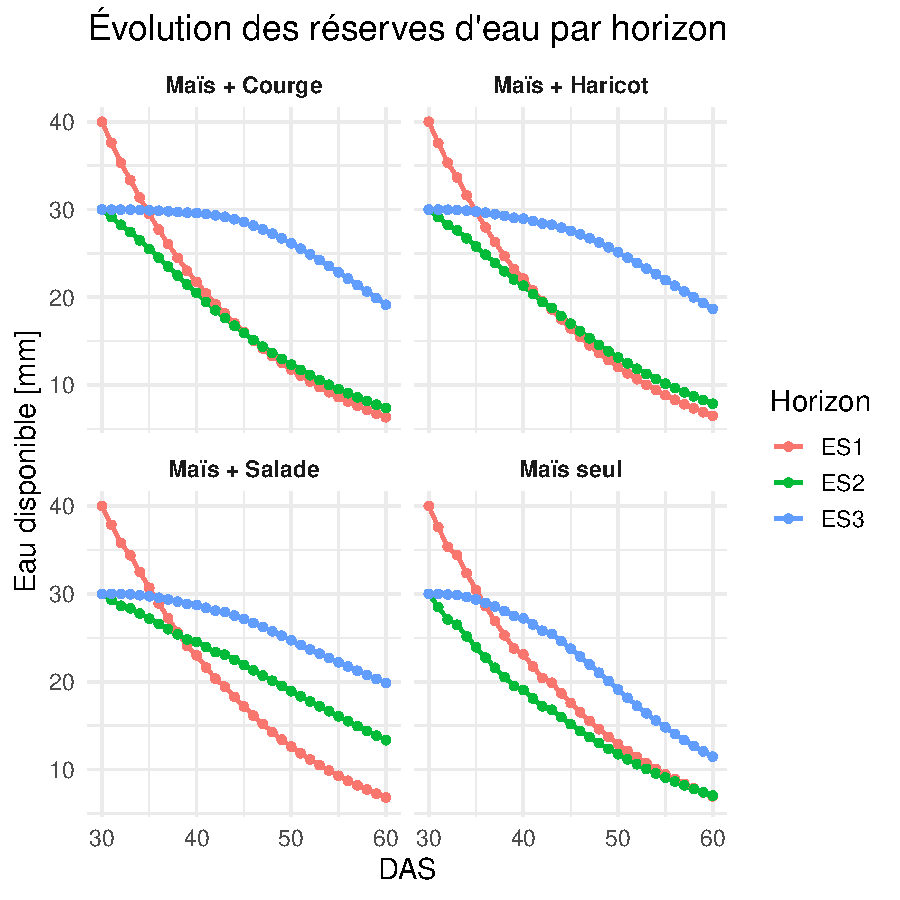
\includegraphics[width=0.7\linewidth]{Rapport_final_Maxime_CORNEZ_files/figure-latex/graphe-es-1} \end{center}

\begin{Shaded}
\begin{Highlighting}[]
\CommentTok{\# 4) Table pour connaitre les niveaux d\textquotesingle{}eau à J60}
\NormalTok{table\_end60 }\OtherTok{\textless{}{-}}\NormalTok{ df\_water\_all }\SpecialCharTok{\%\textgreater{}\%}
  \FunctionTok{filter}\NormalTok{(Jour }\SpecialCharTok{==} \DecValTok{60}\NormalTok{) }\SpecialCharTok{\%\textgreater{}\%}
\NormalTok{  dplyr}\SpecialCharTok{::}\FunctionTok{select}\NormalTok{(Culture, Horizon, Eau\_mm) }\SpecialCharTok{\%\textgreater{}\%}
  \FunctionTok{pivot\_wider}\NormalTok{(}
    \AttributeTok{names\_from  =}\NormalTok{ Horizon,}
    \AttributeTok{values\_from =}\NormalTok{ Eau\_mm}
\NormalTok{  )}

  \CommentTok{\# Affichage de la table}
\NormalTok{  knitr}\SpecialCharTok{::}\FunctionTok{kable}\NormalTok{(}
\NormalTok{    table\_end60,}
    \AttributeTok{col.names =} \FunctionTok{c}\NormalTok{(}\StringTok{"Scénario"}\NormalTok{, }\StringTok{"Horizon 1 (mm)"}\NormalTok{, }\StringTok{"Horizon 2 (mm)"}\NormalTok{, }\StringTok{"Horizon 3 (mm)"}\NormalTok{),}
    \AttributeTok{caption   =} \StringTok{"Eau disponible à J60 par horizon et par scénario"}
\NormalTok{  )}
\end{Highlighting}
\end{Shaded}

\begin{longtable}[]{@{}lrrr@{}}
\caption{Eau disponible à J60 par horizon et par
scénario}\tabularnewline
\toprule\noalign{}
Scénario & Horizon 1 (mm) & Horizon 2 (mm) & Horizon 3 (mm) \\
\midrule\noalign{}
\endfirsthead
\toprule\noalign{}
Scénario & Horizon 1 (mm) & Horizon 2 (mm) & Horizon 3 (mm) \\
\midrule\noalign{}
\endhead
\bottomrule\noalign{}
\endlastfoot
Maïs seul & 6.938496 & 7.020214 & 11.44389 \\
Maïs + Haricot & 6.504094 & 7.874594 & 18.68976 \\
Maïs + Courge & 6.344074 & 7.385780 & 19.15622 \\
Maïs + Salade & 6.804305 & 13.327646 & 19.86248 \\
\end{longtable}

\begin{itemize}
\tightlist
\item
  Épuisement prioritaire de l'horizon 1 :\\
  Dans tous les scénarios, c'est l'horizon superficiel (ES1) qui est le
  plus fortement vidé (de \textasciitilde40 mm à \textasciitilde6--7 mm
  entre J30 et J60). Les différences entre monoculture et intercultures
  sont faibles ici : ES1 résiduel compris entre 6,3 mm pour «
  Maïs+Courge » et 6,9 mm pour le maïs seul, ce qui montre que quel que
  soit le voisin, le maïs exploite d'abord la couche 1.
\item
  Comportement divergent en horizon 2:\\
  En monoculture, ES2 passe de \textasciitilde30 mm à seulement 7 mm
  résiduels à J60, alors que dans l'association maïs--salade, on observe
  13,3 mm dans le deuxième horizon. Les intercultures « maïs+haricot »
  et « maïs+courge » conservent quant à elles \textasciitilde7,4--7,9
  mm. Cela suggère que la salade, vraisemblablement par un schéma
  racinaire plus superficiel ou une moindre demande transpiratoire,
  limite l'extraction dans la zone médiane.
\item
  Réserve profonde dans l'horizon 3 :\\
  Quantitée d'eau résiduelle beaucoup plus élevée en interculture

  \begin{itemize}
  \tightlist
  \item
    Maïs seul : 11,4 mm résiduels
  \item
    Maïs+Haricot : 18,7 mm
  \item
    Maïs+Courge : 19,2 mm
  \item
    Maïs+Salade : 19,9 mm
  \item
    Le maïs en monoculture puise donc beaucoup plus profondément (ne
    laissant que \textasciitilde11 mm) que lorsqu'il est associé à un
    autre couvert. Les intercultures conservent presque 2× plus d'eau
    dans le dernier horizon, signe d'une compétition réduite ou d'une
    complémentarité racinaire (chaque espèce « se partage » moins la
    ressource profonde).
  \end{itemize}
\item
  Implications agronomiques :

  \begin{itemize}
  \tightlist
  \item
    Monoculture : extraction forte et uniforme sur tout le profil,
    risque de stress plus précoce si la recharge est limitée.
  \item
    Intercultures : moindre exploitation des horizons moyens et profonds
    par le maïs, avec une conservation potentielle de la ressource en
    eau pour les stades ultérieurs ou pour l'autre espèce.\\
    L'association maïs--salade est la plus économe en eau médiane et
    profonde, ce qui peut être recherché dans des systèmes à faible
    pluviométrie ou pour limiter le risque d'assèchement rapide.
  \end{itemize}
\end{itemize}

En résumé, si l'horizon 1 est systématiquement drainé en priorité, les
intercultures modulent sensiblement l'exploitation des horizons 2 et 3 :
la monoculture creuse le profil jusqu'au profond, alors que les
coproductions -- et tout particulièrement maïs--salade -- laissent une
part significative de ressource en eau dans les couches moyennes et
profondes.

\begin{Shaded}
\begin{Highlighting}[]
\CommentTok{\# Calcul des statistiques descriptives par culture et horizon}
\NormalTok{df\_stats }\OtherTok{\textless{}{-}}\NormalTok{ df\_water\_all }\SpecialCharTok{\%\textgreater{}\%}
  \FunctionTok{group\_by}\NormalTok{(Culture, Horizon) }\SpecialCharTok{\%\textgreater{}\%}
  \FunctionTok{summarise}\NormalTok{(}
    \AttributeTok{mean\_Eau =} \FunctionTok{mean}\NormalTok{(Eau\_mm),}
    \AttributeTok{sd\_Eau   =} \FunctionTok{sd}\NormalTok{(Eau\_mm),}
    \AttributeTok{.groups  =} \StringTok{"drop"}
\NormalTok{  )}
\FunctionTok{print}\NormalTok{(df\_stats)}
\end{Highlighting}
\end{Shaded}

\begin{verbatim}
## # A tibble: 12 x 4
##    Culture        Horizon mean_Eau sd_Eau
##    <chr>          <chr>      <dbl>  <dbl>
##  1 Maïs + Courge  ES1         18.5  10.0 
##  2 Maïs + Courge  ES2         17.1   7.17
##  3 Maïs + Courge  ES3         26.9   3.49
##  4 Maïs + Haricot ES1         18.7   9.96
##  5 Maïs + Haricot ES2         17.7   6.99
##  6 Maïs + Haricot ES3         26.3   3.64
##  7 Maïs + Salade  ES1         19.3  10.0 
##  8 Maïs + Salade  ES2         21.7   5.03
##  9 Maïs + Salade  ES3         26.2   3.37
## 10 Maïs seul      ES1         19.4   9.85
## 11 Maïs seul      ES2         16.2   6.88
## 12 Maïs seul      ES3         22.4   6.36
\end{verbatim}

L'analyse des statistiques descriptives montre que, quel que soit le
scénario, l'horizon 3 (ES3) conserve systématiquement les volumes d'eau
les plus élevés (μ≈26--27 mm) et les variations les plus faibles (σ≈3--4
mm), ce qui reflète son rôle de réserve profonde moins exploitée par les
racines au cours de la simulation.\\
En surface (ES1), les moyennes oscillent entre 18,5 mm (Maïs + Courge)
et 19,4 mm (Maïs seul), avec des écarts-types relativement importants
(σ≈10 mm) traduisant une forte variabilité journalière due aux
fluctuations climatiques et à l'intensité d'extraction racinaire.\\
Pour l'horizon intermédiaire (ES2), on observe un léger gain d'eau
disponible dans le scénario Maïs + Salade (μ=21,7 mm) par rapport aux
autres (μ≈17 mm), suggérant une complémentarité racinaire qui réduit la
concurrence sur ce niveau.\\
Enfin, le scénario Maïs seul présente la plus faible réserve moyenne en
ES2 (16,2 mm), signe qu'en monoculture le sol intermédiaire est plus
fortement exploité. Ces résultats confirment l'impact des associations
culturales sur la distribution spatiale de l'extraction racinaire et
mettent en évidence une meilleure préservation des ressources en
interculture, notamment pour les horizons moyens et profonds.

\subsubsection{Évolution du ratio Offre/Demande
(O/D)}\label{uxe9volution-du-ratio-offredemande-od}

\begin{Shaded}
\begin{Highlighting}[]
\CommentTok{\# 1) Concaténation de tous les scénarios}
\NormalTok{df\_od\_all }\OtherTok{\textless{}{-}} \FunctionTok{bind\_rows}\NormalTok{(}
\NormalTok{  resultat\_mais               }\SpecialCharTok{\%\textgreater{}\%} \FunctionTok{mutate}\NormalTok{(}\AttributeTok{Scenario =} \StringTok{"Maïs seul"}\NormalTok{)}\SpecialCharTok{\%\textgreater{}\%} \FunctionTok{rename}\NormalTok{(}\AttributeTok{sdratio1 =}\NormalTok{ O\_D),}
\NormalTok{  resultats\_mais\_haricot      }\SpecialCharTok{\%\textgreater{}\%} \FunctionTok{mutate}\NormalTok{(}\AttributeTok{Scenario =} \StringTok{"Maïs + Haricot"}\NormalTok{),}
\NormalTok{  resultats\_mais\_courge       }\SpecialCharTok{\%\textgreater{}\%} \FunctionTok{mutate}\NormalTok{(}\AttributeTok{Scenario =} \StringTok{"Maïs + Courge"}\NormalTok{),}
\NormalTok{  resultats\_mais\_salade       }\SpecialCharTok{\%\textgreater{}\%} \FunctionTok{mutate}\NormalTok{(}\AttributeTok{Scenario =} \StringTok{"Maïs + Salade"}\NormalTok{)}
\NormalTok{) }\SpecialCharTok{\%\textgreater{}\%}
  \FunctionTok{pivot\_longer}\NormalTok{(}
    \AttributeTok{cols =} \FunctionTok{c}\NormalTok{(}\FunctionTok{starts\_with}\NormalTok{(}\StringTok{"sdratio"}\NormalTok{)),}
    \AttributeTok{names\_to  =} \StringTok{"Culture"}\NormalTok{,}
    \AttributeTok{values\_to =} \StringTok{"OD"}\NormalTok{,}
    \AttributeTok{values\_drop\_na =} \ConstantTok{TRUE}
\NormalTok{  )}

\CommentTok{\# 3) Tracé en facettes}
\FunctionTok{ggplot}\NormalTok{(df\_od\_all, }\FunctionTok{aes}\NormalTok{(}\AttributeTok{x =}\NormalTok{ Jour, }\AttributeTok{y =}\NormalTok{ OD, }\AttributeTok{color =}\NormalTok{ Culture)) }\SpecialCharTok{+}
  \FunctionTok{geom\_hline}\NormalTok{(}\AttributeTok{yintercept =} \DecValTok{1}\NormalTok{, }\AttributeTok{linetype =} \StringTok{"dashed"}\NormalTok{, }\AttributeTok{color =} \StringTok{"black"}\NormalTok{) }\SpecialCharTok{+}
  \FunctionTok{geom\_line}\NormalTok{(}\AttributeTok{size =} \FloatTok{0.8}\NormalTok{) }\SpecialCharTok{+}
  \FunctionTok{geom\_point}\NormalTok{(}\AttributeTok{size =} \FloatTok{1.5}\NormalTok{) }\SpecialCharTok{+}
  \FunctionTok{facet\_wrap}\NormalTok{(}\SpecialCharTok{\textasciitilde{}}\NormalTok{ Scenario, }\AttributeTok{ncol =} \DecValTok{2}\NormalTok{) }\SpecialCharTok{+}
  \FunctionTok{labs}\NormalTok{(}
    \AttributeTok{title =} \StringTok{"Évolution des ratios Offre/Demande (O/D)"}\NormalTok{,}
    \AttributeTok{x     =} \StringTok{"DAS"}\NormalTok{,}
    \AttributeTok{y     =} \StringTok{"O/D"}\NormalTok{,}
    \AttributeTok{color =} \StringTok{"Culture"}
\NormalTok{  ) }\SpecialCharTok{+}
  \FunctionTok{theme\_minimal}\NormalTok{(}\AttributeTok{base\_size =} \DecValTok{14}\NormalTok{) }\SpecialCharTok{+}
  \FunctionTok{theme}\NormalTok{(}\AttributeTok{strip.text =} \FunctionTok{element\_text}\NormalTok{(}\AttributeTok{face =} \StringTok{"bold"}\NormalTok{))}
\end{Highlighting}
\end{Shaded}

\begin{center}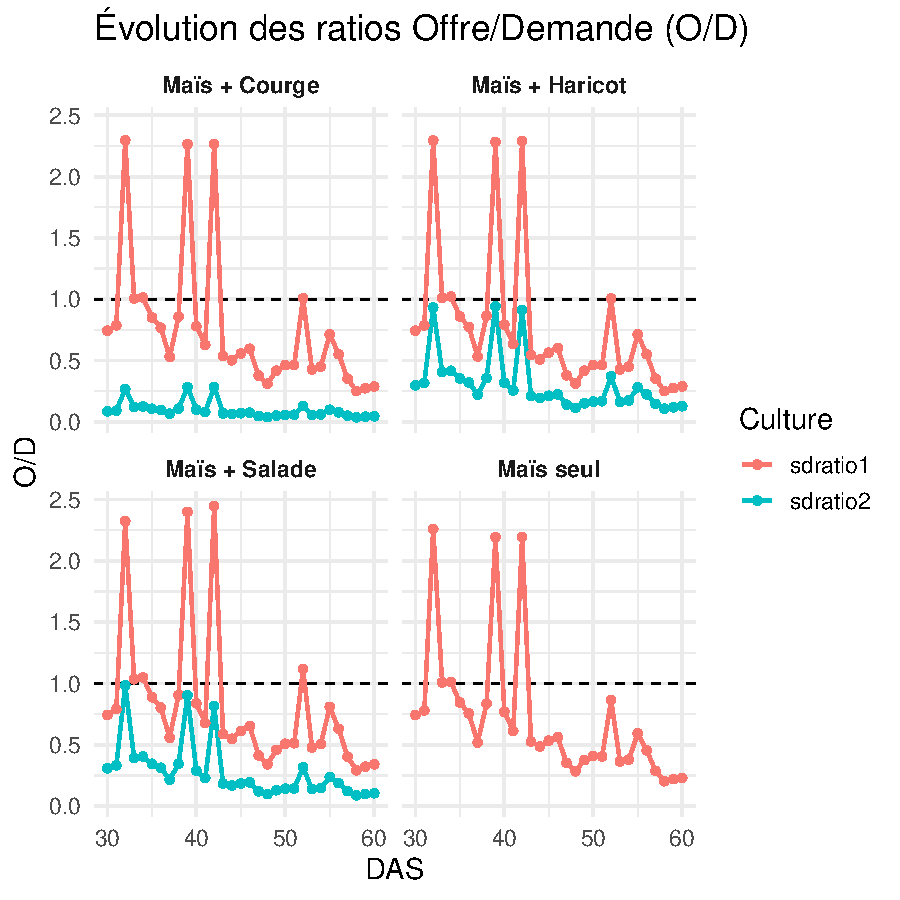
\includegraphics[width=0.7\linewidth]{Rapport_final_Maxime_CORNEZ_files/figure-latex/graphe-od-facets-1} \end{center}

Il est visible que, dans tous les scénarios, le ratio O/D pour la
culture principale (courbe « sdratio1 », en rouge) démarre souvent
au-dessus de 1 (offre abondante), mais chute plusieurs fois en dessous
de 1 à partir du stade intermédiaire (DAS 35--40), témoignant d'épisodes
transitoires de stress hydrique. La culture associée (courbe « sdratio2
», en bleu) reste presque toujours en dessous de 1, soulignant sa
pression compétitive plus faible ou son enracinement plus superficiel.
Il y a peu de différences entre les scénarios, cela est surement du à
l'hypothèse que les deux cultures n'entrent pas en compétion pour la
lumière, de fait elles suivent la même dynamique de O/D en fonction de
la météo.

\begin{longtable}[]{@{}lr@{}}
\caption{Tableau 1 : Jours où le ratio Offre/Demande (O/D) est inférieur
à 1}\tabularnewline
\toprule\noalign{}
Scénario & Nombre de jours de stress hydrique \\
\midrule\noalign{}
\endfirsthead
\toprule\noalign{}
Scénario & Nombre de jours de stress hydrique \\
\midrule\noalign{}
\endhead
\bottomrule\noalign{}
\endlastfoot
Maïs seul & 26 \\
Maïs + Haricot & 31 \\
Maïs + Courge & 31 \\
Maïs + Salade & 31 \\
\end{longtable}

Dans les trois intercultures, la répartition de l'eau entre les deux
espèces conduit à un léger surcroît de jours de déficit pour le maïs (et
globalement pour le système), car chacune prélève dans le même profil.
L'interaction racinaire diminue l'offre relative disponible, même si le
sol contient encore de l'eau. Cependant, cinq jours de déficit
supplémentaires sur une période d'étude de soixante jours ne sont pas
signficatifs.

\subsubsection{Évolution de la
biomasse}\label{uxe9volution-de-la-biomasse}

\begin{Shaded}
\begin{Highlighting}[]
\CommentTok{\# 1) Concaténation de tous les scénarios}
\NormalTok{df\_biom\_all }\OtherTok{\textless{}{-}} \FunctionTok{bind\_rows}\NormalTok{(}
\NormalTok{  resultat\_mais          }\SpecialCharTok{\%\textgreater{}\%} \FunctionTok{mutate}\NormalTok{(}\AttributeTok{Scenario =} \StringTok{"Maïs seul"}\NormalTok{)}\SpecialCharTok{\%\textgreater{}\%} \FunctionTok{rename}\NormalTok{(}\AttributeTok{Biomasse\_cum1 =}\NormalTok{ Biomasse\_cum),}
\NormalTok{  resultats\_mais\_haricot }\SpecialCharTok{\%\textgreater{}\%} \FunctionTok{mutate}\NormalTok{(}\AttributeTok{Scenario =} \StringTok{"Maïs + Haricot"}\NormalTok{),}
\NormalTok{  resultats\_mais\_courge  }\SpecialCharTok{\%\textgreater{}\%} \FunctionTok{mutate}\NormalTok{(}\AttributeTok{Scenario =} \StringTok{"Maïs + Courge"}\NormalTok{),}
\NormalTok{  resultats\_mais\_salade  }\SpecialCharTok{\%\textgreater{}\%} \FunctionTok{mutate}\NormalTok{(}\AttributeTok{Scenario =} \StringTok{"Maïs + Salade"}\NormalTok{)}
\NormalTok{) }\SpecialCharTok{\%\textgreater{}\%}
  \CommentTok{\# 2) Pivot\_longer sur les colonnes de biomasse cumulée}
  \FunctionTok{pivot\_longer}\NormalTok{(}
    \AttributeTok{cols           =} \FunctionTok{starts\_with}\NormalTok{(}\StringTok{"Biomasse\_cum"}\NormalTok{),}
    \AttributeTok{names\_to       =} \StringTok{"Culture"}\NormalTok{,}
    \AttributeTok{values\_to      =} \StringTok{"Biomasse\_gm2"}\NormalTok{,}
    \AttributeTok{values\_drop\_na =} \ConstantTok{TRUE}    \CommentTok{\# on ne garde que les valeurs existantes}
\NormalTok{  )}

\CommentTok{\# 3) Tracé en facettes}
\FunctionTok{ggplot}\NormalTok{(df\_biom\_all, }\FunctionTok{aes}\NormalTok{(}\AttributeTok{x =}\NormalTok{ Jour, }\AttributeTok{y =}\NormalTok{ Biomasse\_gm2, }\AttributeTok{color =}\NormalTok{ Culture)) }\SpecialCharTok{+}
  \FunctionTok{geom\_line}\NormalTok{(}\AttributeTok{size =} \FloatTok{0.8}\NormalTok{) }\SpecialCharTok{+}
  \FunctionTok{geom\_point}\NormalTok{(}\AttributeTok{size =} \FloatTok{1.5}\NormalTok{) }\SpecialCharTok{+}
  \FunctionTok{facet\_wrap}\NormalTok{(}\SpecialCharTok{\textasciitilde{}}\NormalTok{ Scenario, }\AttributeTok{ncol =} \DecValTok{2}\NormalTok{) }\SpecialCharTok{+}
  \FunctionTok{labs}\NormalTok{(}
    \AttributeTok{title =} \StringTok{"Évolution de la biomasse cumulée selon le scénario"}\NormalTok{,}
    \AttributeTok{x     =} \StringTok{"DAS"}\NormalTok{,}
    \AttributeTok{y     =} \StringTok{"Biomasse cumulée (g·m⁻²)"}\NormalTok{,}
    \AttributeTok{color =} \StringTok{"Culture"}
\NormalTok{  ) }\SpecialCharTok{+}
  \FunctionTok{theme\_minimal}\NormalTok{(}\AttributeTok{base\_size =} \DecValTok{14}\NormalTok{) }\SpecialCharTok{+}
  \FunctionTok{theme}\NormalTok{(}\AttributeTok{strip.text =} \FunctionTok{element\_text}\NormalTok{(}\AttributeTok{face =} \StringTok{"bold"}\NormalTok{))}
\end{Highlighting}
\end{Shaded}

\begin{center}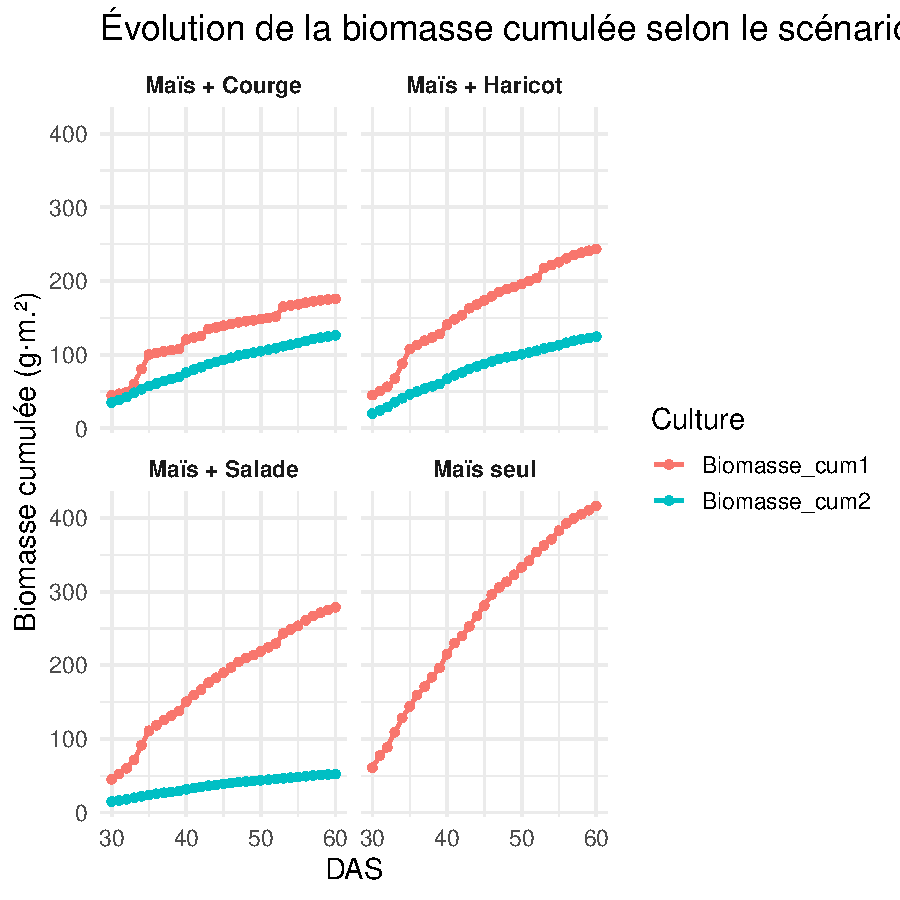
\includegraphics[width=0.7\linewidth]{Rapport_final_Maxime_CORNEZ_files/figure-latex/graphe-biomasse-1} \end{center}

\begin{longtable}[]{@{}
  >{\raggedright\arraybackslash}p{(\linewidth - 8\tabcolsep) * \real{0.1240}}
  >{\raggedleft\arraybackslash}p{(\linewidth - 8\tabcolsep) * \real{0.2314}}
  >{\raggedleft\arraybackslash}p{(\linewidth - 8\tabcolsep) * \real{0.2479}}
  >{\raggedleft\arraybackslash}p{(\linewidth - 8\tabcolsep) * \real{0.1901}}
  >{\raggedleft\arraybackslash}p{(\linewidth - 8\tabcolsep) * \real{0.2066}}@{}}
\caption{Tableau : biomasse à J60 et pentes journalières, par
scénario}\tabularnewline
\toprule\noalign{}
\begin{minipage}[b]{\linewidth}\raggedright
Scénario
\end{minipage} & \begin{minipage}[b]{\linewidth}\raggedleft
Biomasse maïs à J60 (g·m⁻²)
\end{minipage} & \begin{minipage}[b]{\linewidth}\raggedleft
Biomasse totale à J60 (g·m⁻²)
\end{minipage} & \begin{minipage}[b]{\linewidth}\raggedleft
Pente maïs (g·m⁻²·j⁻¹)
\end{minipage} & \begin{minipage}[b]{\linewidth}\raggedleft
Pente totale (g·m⁻²·j⁻¹)
\end{minipage} \\
\midrule\noalign{}
\endfirsthead
\toprule\noalign{}
\begin{minipage}[b]{\linewidth}\raggedright
Scénario
\end{minipage} & \begin{minipage}[b]{\linewidth}\raggedleft
Biomasse maïs à J60 (g·m⁻²)
\end{minipage} & \begin{minipage}[b]{\linewidth}\raggedleft
Biomasse totale à J60 (g·m⁻²)
\end{minipage} & \begin{minipage}[b]{\linewidth}\raggedleft
Pente maïs (g·m⁻²·j⁻¹)
\end{minipage} & \begin{minipage}[b]{\linewidth}\raggedleft
Pente totale (g·m⁻²·j⁻¹)
\end{minipage} \\
\midrule\noalign{}
\endhead
\bottomrule\noalign{}
\endlastfoot
Maïs + Courge & 175.8 & 302.0 & 4.169 & 7.188 \\
Maïs + Haricot & 243.6 & 367.9 & 6.513 & 9.974 \\
Maïs + Salade & 278.7 & 331.0 & 7.696 & 8.943 \\
Maïs seul & 416.2 & 416.2 & 11.978 & 11.978 \\
\end{longtable}

\begin{itemize}
\item
  \textbf{Monoculture de maïs :\\
  }La production cumulée atteint \textbf{416,2 g·m⁻²} à 60 DAS, avec une
  pente journalière de \textbf{11,978 g·m⁻²·j⁻¹}, la plus forte de tous
  les scénarios. En l'absence de compétition racinaire et foliaire,
  toute la radiation et l'eau disponible profitent exclusivement au
  maïs, lui permettant de synthétiser plus et plus rapidement de la
  biomasse.
\item
  \textbf{Maïs + Courge:}

  \begin{itemize}
  \item
    Maïs : \textbf{175,8 g·m⁻²} à J 60, pente = 4,169 g·m⁻²·j⁻¹
    =\textgreater{} \textbf{--57,8 \%} par rapport à la monoculture
  \item
    Courge : 302,0--175,8 = 126,2 g·m⁻², pente = 7,188--4,169 = 3,019
    g·m⁻²·j⁻¹
  \end{itemize}

  La courge capte une part significative des ressources (≈30 \% de la
  biomasse totale), au prix d'une réduction d'environ 58 \% de la
  production de maïs.
\item
  \textbf{Maïs + Haricot}

  \begin{itemize}
  \item
    Maïs : \textbf{243,6 g·m⁻²} à J 60, pente = 6,513 g·m⁻²·j⁻¹
    =\textgreater{} \textbf{--41,5 \%} par rapport monoculture
  \item
    Haricot : 367,9--243,6 = 124,3 g·m⁻², pente = 9,974--6,513 = 3,461
    g·m⁻²·j⁻¹
  \end{itemize}

  Le haricot capte moins de ressources de la maïs du fait de son VPR
  plus faible, cependant pour produire une biomasse égale à celle du
  maïs, il a besoin de plus d'eau en raison de son TEc
\item
  \textbf{Maïs + Salade}

  \begin{itemize}
  \item
    Maïs : 278,7 g·m⁻² à J 60, pente = 7,696 g·m⁻²·j⁻¹ =\textgreater{}
    --33,1 \% par rapport à la monoculture
  \item
    Salade : 331,0--278,7 = 52,3 g·m⁻², pente = 8,943--7,696 = 1,247
    g·m⁻²·j⁻¹
  \end{itemize}
\end{itemize}

La salade, avec un VPR faible, prélève peu d'eau : elle limite donc
modérément la croissance du maïs (-33,1 \%), mais sa propre biomasse
reste très réduite.

En résumé :

\begin{itemize}
\item
  \textbf{Le rendement maximum} : en monoculture, le maïs montre la plus
  forte pente et la plus grande biomasse (416 g·m⁻²).
\item
  \textbf{Les compromis de l'interculture} : toute espèce associée capte
  une part non négligeable des ressources, diminuant la production du
  maïs :

  \begin{enumerate}
  \def\labelenumi{\arabic{enumi}.}
  \item
    \textbf{Salade} : moindre prélèvement (--33 \% de maïs), mais
    biomasse associative très faible.
  \item
    \textbf{Haricot} : biomasse associative ≈ 124 g·m⁻², réduction du
    maïs ≈ 42 \%.
  \item
    \textbf{Courge} : biomasse associative ≈ 126 g·m⁻², réduction du
    maïs ≈ 58 \%.
  \end{enumerate}
\end{itemize}

\textbf{Le choix de l'associé} :\\
Le choix de la stratégie culturale doit avant tout être guidé par
l'objectif agronomique et économique recherché. Si l'enjeu principal est
\textbf{de maximiser le rendement de la sole de maïs}, la monoculture ou
l'association avec une culture de faible compétition hydrique, comme la
salade, se révèle la plus efficace : la courbe de croissance du maïs y
conserve la pente la plus élevée, et la biomasse cumulée à 60 DAS est
maximale, garantissant un gain de matière sèche par unité de surface
optimal.

En revanche, si l'on vise un \textbf{rendement global du système plus
équilibré}, incluant la production de la culture secondaire, alors des
couvertures interculturelles plus vigoureuses -- haricot ou courge --
deviennent pertinentes. Ces associations réduisent certes la production
de maïs de 40 à 60 \%, mais elles augmentent la productivité totale de
la parcelle, diversifient les débouchés (graines, légumes,
fourrage\ldots) et apportent des \textbf{services écosystémiques}
précieux. Par exemple, le haricot, en tant que légumineuse, contribue à
la \textbf{fixation atmosphérique d'azote}, réduisant les besoins en
fertilisation et améliorant la fertilité du sol pour les cultures
suivantes. De même, la courge, par son feuillage étalé et son système
racinaire complémentaire, peut limiter l'érosion et maintenir l'humidité
du sol en période chaude.

Ainsi, la décision revient à arbitrer entre l'intensification de la
production de maïs (mono ou avec salade) pour maximiser le rendement
unitaire et la rentabilité à court terme et l'optimisation du rendement
de système (maïs + haricot ou courge) pour valoriser des coproduits,
améliorer la durabilité des sols et réduire l'empreinte
environnementale, au détriment d'une baisse partielle du rendement
maïs.\\
Dans tous les cas, il convient d'intégrer ces choix dans une rotation
culturale plus large, tenant compte des besoins en azote, de la
structure du sol, des conditions climatiques et des objectifs
économiques de la ferme.

\subsubsection{Évolution de la quantité d'eau
transpirée}\label{uxe9volution-de-la-quantituxe9-deau-transpiruxe9e}

\begin{Shaded}
\begin{Highlighting}[]
\CommentTok{\# 1) Préparer chaque scénario avec deux colonnes Transpiration1\_cum et Transpiration2\_cum}

\CommentTok{\#   Maïs seul : une seule culture → Transpiration2\_cum = NA}
\NormalTok{df\_mais\_seul }\OtherTok{\textless{}{-}}\NormalTok{ resultat\_mais }\SpecialCharTok{\%\textgreater{}\%}
  \FunctionTok{mutate}\NormalTok{(}
    \AttributeTok{Transpiration1\_cum =} \FunctionTok{cumsum}\NormalTok{(Transpiration),}
    \AttributeTok{Transpiration2\_cum =} \ConstantTok{NA\_real\_}\NormalTok{,}
    \AttributeTok{Scenario =} \StringTok{"Maïs seul"}
\NormalTok{  ) }\SpecialCharTok{\%\textgreater{}\%}
\NormalTok{  dplyr}\SpecialCharTok{::}\FunctionTok{select}\NormalTok{(Scenario, Jour, Transpiration1\_cum, Transpiration2\_cum)}

\CommentTok{\#   Maïs + Haricot}
\NormalTok{df\_mais\_haricot }\OtherTok{\textless{}{-}}\NormalTok{ resultats\_mais\_haricot }\SpecialCharTok{\%\textgreater{}\%}
  \FunctionTok{mutate}\NormalTok{(}
    \AttributeTok{Transpiration1\_cum =} \FunctionTok{cumsum}\NormalTok{(Transpiration1),}
    \AttributeTok{Transpiration2\_cum =} \FunctionTok{cumsum}\NormalTok{(Transpiration2),}
    \AttributeTok{Scenario =} \StringTok{"Maïs + Haricot"}
\NormalTok{  ) }\SpecialCharTok{\%\textgreater{}\%}
\NormalTok{  dplyr}\SpecialCharTok{::}\FunctionTok{select}\NormalTok{(Scenario, Jour, Transpiration1\_cum, Transpiration2\_cum)}

\CommentTok{\#   Maïs + Courge}
\NormalTok{df\_mais\_courge }\OtherTok{\textless{}{-}}\NormalTok{ resultats\_mais\_courge }\SpecialCharTok{\%\textgreater{}\%}
  \FunctionTok{mutate}\NormalTok{(}
    \AttributeTok{Transpiration1\_cum =} \FunctionTok{cumsum}\NormalTok{(Transpiration1),}
    \AttributeTok{Transpiration2\_cum =} \FunctionTok{cumsum}\NormalTok{(Transpiration2),}
    \AttributeTok{Scenario =} \StringTok{"Maïs + Courge"}
\NormalTok{  ) }\SpecialCharTok{\%\textgreater{}\%}
\NormalTok{  dplyr}\SpecialCharTok{::}\FunctionTok{select}\NormalTok{(Scenario, Jour, Transpiration1\_cum, Transpiration2\_cum)}

\CommentTok{\#   Maïs + Salade}
\NormalTok{df\_mais\_salade }\OtherTok{\textless{}{-}}\NormalTok{ resultats\_mais\_salade }\SpecialCharTok{\%\textgreater{}\%}
  \FunctionTok{mutate}\NormalTok{(}
    \AttributeTok{Transpiration1\_cum =} \FunctionTok{cumsum}\NormalTok{(Transpiration1),}
    \AttributeTok{Transpiration2\_cum =} \FunctionTok{cumsum}\NormalTok{(Transpiration2),}
    \AttributeTok{Scenario =} \StringTok{"Maïs + Salade"}
\NormalTok{  ) }\SpecialCharTok{\%\textgreater{}\%}
\NormalTok{  dplyr}\SpecialCharTok{::}\FunctionTok{select}\NormalTok{(Scenario, Jour, Transpiration1\_cum, Transpiration2\_cum)}

\CommentTok{\# 2) Concaténer et passer en format long, en supprimant les NA}
\NormalTok{df\_transpi\_all }\OtherTok{\textless{}{-}} \FunctionTok{bind\_rows}\NormalTok{(}
\NormalTok{  df\_mais\_seul,}
\NormalTok{  df\_mais\_haricot,}
\NormalTok{  df\_mais\_courge,}
\NormalTok{  df\_mais\_salade}
\NormalTok{) }\SpecialCharTok{\%\textgreater{}\%}
  \FunctionTok{pivot\_longer}\NormalTok{(}
    \AttributeTok{cols           =} \FunctionTok{c}\NormalTok{(Transpiration1\_cum, Transpiration2\_cum),}
    \AttributeTok{names\_to       =} \StringTok{"Culture"}\NormalTok{,}
    \AttributeTok{values\_to      =} \StringTok{"Transpiration\_cum"}\NormalTok{,}
    \AttributeTok{values\_drop\_na =} \ConstantTok{TRUE}
\NormalTok{  )}

\CommentTok{\# 3) Tracé en facettes}
\FunctionTok{ggplot}\NormalTok{(df\_transpi\_all, }\FunctionTok{aes}\NormalTok{(}\AttributeTok{x =}\NormalTok{ Jour, }\AttributeTok{y =}\NormalTok{ Transpiration\_cum, }\AttributeTok{color =}\NormalTok{ Culture)) }\SpecialCharTok{+}
  \FunctionTok{geom\_line}\NormalTok{(}\AttributeTok{size =} \FloatTok{0.8}\NormalTok{) }\SpecialCharTok{+}
  \FunctionTok{geom\_point}\NormalTok{(}\AttributeTok{size =} \FloatTok{1.5}\NormalTok{) }\SpecialCharTok{+}
  \FunctionTok{facet\_wrap}\NormalTok{(}\SpecialCharTok{\textasciitilde{}}\NormalTok{ Scenario, }\AttributeTok{ncol =} \DecValTok{2}\NormalTok{) }\SpecialCharTok{+}
  \FunctionTok{labs}\NormalTok{(}
    \AttributeTok{title =} \StringTok{"Transpiration cumulée par scénario"}\NormalTok{,}
    \AttributeTok{x     =} \StringTok{"DAS"}\NormalTok{,}
    \AttributeTok{y     =} \StringTok{"Transpiration cumulée [mm]"}\NormalTok{,}
    \AttributeTok{color =} \StringTok{"Culture"}
\NormalTok{  ) }\SpecialCharTok{+}
  \FunctionTok{theme\_minimal}\NormalTok{(}\AttributeTok{base\_size =} \DecValTok{14}\NormalTok{) }\SpecialCharTok{+}
  \FunctionTok{theme}\NormalTok{(}\AttributeTok{strip.text =} \FunctionTok{element\_text}\NormalTok{(}\AttributeTok{face =} \StringTok{"bold"}\NormalTok{))}
\end{Highlighting}
\end{Shaded}

\begin{center}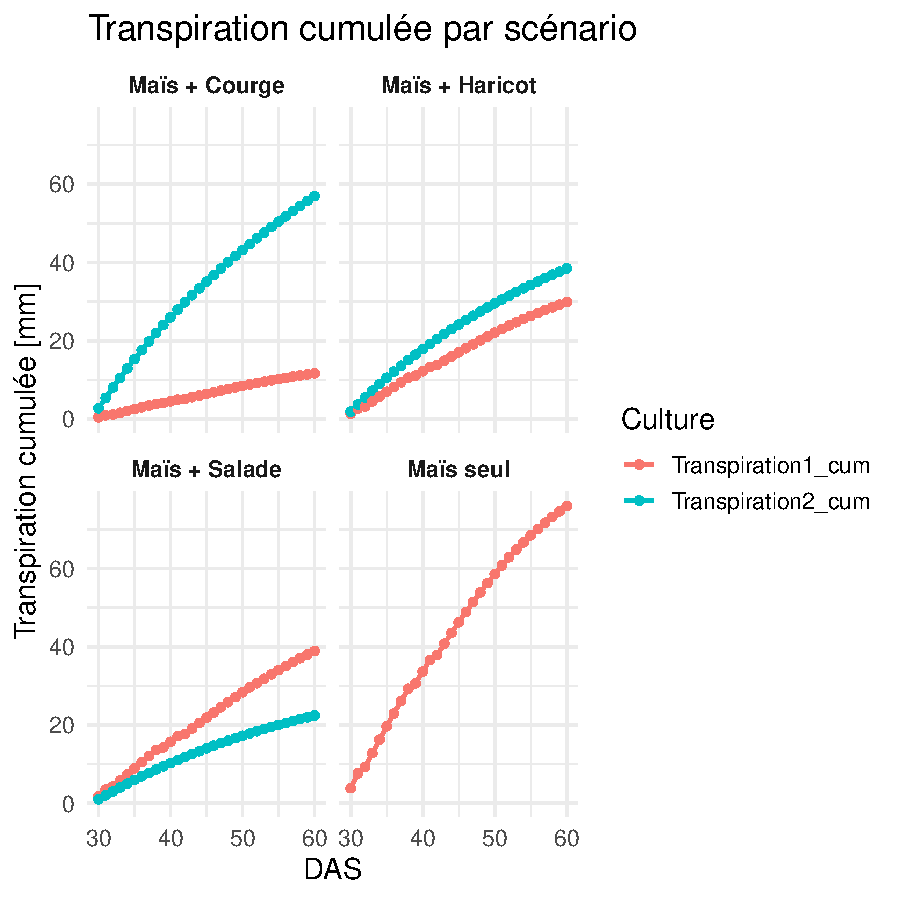
\includegraphics[width=0.7\linewidth]{Rapport_final_Maxime_CORNEZ_files/figure-latex/graphe-transpi-cum-1} \end{center}

\begin{Shaded}
\begin{Highlighting}[]
\CommentTok{\# 1) Préparer WUE (Water Use Efficiency) cumulée pour chaque scénario}
\NormalTok{make\_wue\_df }\OtherTok{\textless{}{-}} \ControlFlowTok{function}\NormalTok{(df, scenario, }\AttributeTok{is\_duo=}\ConstantTok{FALSE}\NormalTok{) \{}
  \ControlFlowTok{if}\NormalTok{ (}\SpecialCharTok{!}\NormalTok{is\_duo) \{}
\NormalTok{    df2 }\OtherTok{\textless{}{-}}\NormalTok{ df }\SpecialCharTok{\%\textgreater{}\%}
      \FunctionTok{mutate}\NormalTok{(}
        \AttributeTok{Biomasse\_cum =}\NormalTok{ Biomasse\_cum,}
        \AttributeTok{Transp\_cum   =} \FunctionTok{cumsum}\NormalTok{(Transpiration)}
\NormalTok{      ) }\SpecialCharTok{\%\textgreater{}\%}
\NormalTok{      dplyr}\SpecialCharTok{::}\FunctionTok{select}\NormalTok{(Jour, Biomasse\_cum, Transp\_cum) }\SpecialCharTok{\%\textgreater{}\%}
      \FunctionTok{mutate}\NormalTok{(}\AttributeTok{Scenario =}\NormalTok{ scenario)}
\NormalTok{  \} }\ControlFlowTok{else}\NormalTok{ \{}
\NormalTok{    df2 }\OtherTok{\textless{}{-}}\NormalTok{ df }\SpecialCharTok{\%\textgreater{}\%}
      \FunctionTok{mutate}\NormalTok{(}
        \AttributeTok{Biomasse\_cum =}\NormalTok{ Biomasse\_cum1 }\SpecialCharTok{+}\NormalTok{ Biomasse\_cum2,}
        \AttributeTok{Transp\_cum   =} \FunctionTok{cumsum}\NormalTok{(Transpiration1) }\SpecialCharTok{+} \FunctionTok{cumsum}\NormalTok{(Transpiration2)}
\NormalTok{      ) }\SpecialCharTok{\%\textgreater{}\%}
\NormalTok{      dplyr}\SpecialCharTok{::}\FunctionTok{select}\NormalTok{(Jour, Biomasse\_cum, Transp\_cum) }\SpecialCharTok{\%\textgreater{}\%}
      \FunctionTok{mutate}\NormalTok{(}\AttributeTok{Scenario =}\NormalTok{ scenario)}
\NormalTok{  \}}
\NormalTok{  df2 }\SpecialCharTok{\%\textgreater{}\%}
    \FunctionTok{mutate}\NormalTok{(}\AttributeTok{WUE =}\NormalTok{ Biomasse\_cum }\SpecialCharTok{/}\NormalTok{ Transp\_cum)}
\NormalTok{\}}

\NormalTok{wue\_all }\OtherTok{\textless{}{-}} \FunctionTok{bind\_rows}\NormalTok{(}
  \FunctionTok{make\_wue\_df}\NormalTok{(resultat\_mais,               }\StringTok{"Maïs seul"}\NormalTok{,      }\ConstantTok{FALSE}\NormalTok{),}
  \FunctionTok{make\_wue\_df}\NormalTok{(resultats\_mais\_haricot,      }\StringTok{"Maïs + Haricot"}\NormalTok{, }\ConstantTok{TRUE}\NormalTok{),}
  \FunctionTok{make\_wue\_df}\NormalTok{(resultats\_mais\_courge,       }\StringTok{"Maïs + Courge"}\NormalTok{,  }\ConstantTok{TRUE}\NormalTok{),}
  \FunctionTok{make\_wue\_df}\NormalTok{(resultats\_mais\_salade,       }\StringTok{"Maïs + Salade"}\NormalTok{,  }\ConstantTok{TRUE}\NormalTok{)}
\NormalTok{)}

\CommentTok{\# a) WUE au cours du temps}
\FunctionTok{ggplot}\NormalTok{(wue\_all, }\FunctionTok{aes}\NormalTok{(}\AttributeTok{x =}\NormalTok{ Jour, }\AttributeTok{y =}\NormalTok{ WUE, }\AttributeTok{color =}\NormalTok{ Scenario)) }\SpecialCharTok{+}
  \FunctionTok{geom\_line}\NormalTok{() }\SpecialCharTok{+} \FunctionTok{geom\_point}\NormalTok{() }\SpecialCharTok{+}
  \FunctionTok{labs}\NormalTok{(}\AttributeTok{title=}\StringTok{"WUE cumulée (g·m⁻² / mm)"}\NormalTok{, }\AttributeTok{x=}\StringTok{"DAS"}\NormalTok{, }\AttributeTok{y=}\StringTok{"WUE"}\NormalTok{) }\SpecialCharTok{+}
  \FunctionTok{theme\_minimal}\NormalTok{()}
\end{Highlighting}
\end{Shaded}

\begin{center}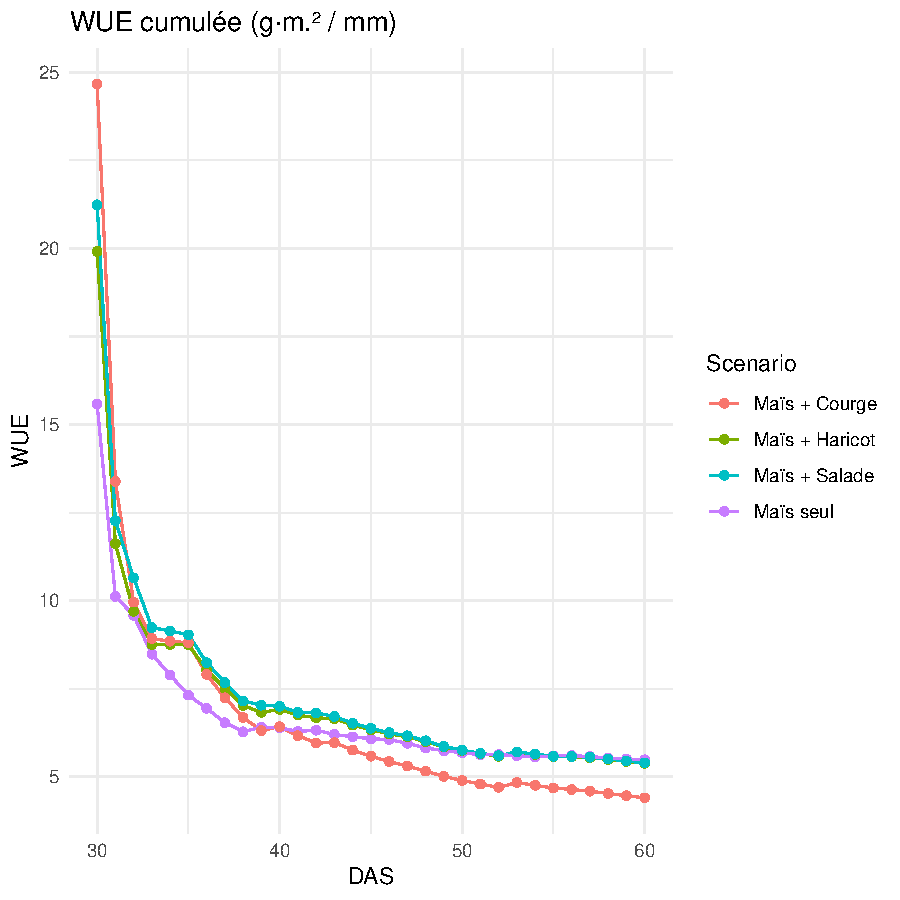
\includegraphics[width=0.7\linewidth]{Rapport_final_Maxime_CORNEZ_files/figure-latex/WUE-1} \end{center}

\begin{Shaded}
\begin{Highlighting}[]
\CommentTok{\# b) table des valeurs de WUE à J60}
\NormalTok{wue\_J60 }\OtherTok{\textless{}{-}}\NormalTok{ wue\_all }\SpecialCharTok{\%\textgreater{}\%}
  \FunctionTok{filter}\NormalTok{(Jour }\SpecialCharTok{==} \DecValTok{60}\NormalTok{) }\SpecialCharTok{\%\textgreater{}\%}
\NormalTok{  dplyr}\SpecialCharTok{::}\FunctionTok{select}\NormalTok{(Scenario, WUE) }\SpecialCharTok{\%\textgreater{}\%}
  \FunctionTok{arrange}\NormalTok{(}\FunctionTok{desc}\NormalTok{(WUE))}

\NormalTok{knitr}\SpecialCharTok{::}\FunctionTok{kable}\NormalTok{(}
\NormalTok{  wue\_J60,}
  \AttributeTok{col.names =} \FunctionTok{c}\NormalTok{(}\StringTok{"Scénario"}\NormalTok{, }\StringTok{"WUE à J60 (g·m2/mm)"}\NormalTok{),}
  \AttributeTok{caption   =} \StringTok{"Tableau : Water Use Efficiency cumulée au jour 60"}
\NormalTok{)}
\end{Highlighting}
\end{Shaded}

\begin{longtable}[]{@{}lr@{}}
\caption{Tableau : Water Use Efficiency cumulée au jour
60}\tabularnewline
\toprule\noalign{}
Scénario & WUE à J60 (g·m2/mm) \\
\midrule\noalign{}
\endfirsthead
\toprule\noalign{}
Scénario & WUE à J60 (g·m2/mm) \\
\midrule\noalign{}
\endhead
\bottomrule\noalign{}
\endlastfoot
Maïs seul & 5.480513 \\
Maïs + Salade & 5.392999 \\
Maïs + Haricot & 5.381363 \\
Maïs + Courge & 4.400653 \\
\end{longtable}

Le Water Use Efficiency (WUE) est défini comme le rapport entre la
biomasse cumulée produite et l'eau transpirée :
\(\mathrm{WUE} = \frac{\sum B}{T}\) (Rouphael and Colla 2005)

On distingue deux phases dans l'évolution du WUE en fonction du DAS :

\begin{enumerate}
\def\labelenumi{\arabic{enumi}.}
\item
  \textbf{Phase initiale (30--35 DAS)\\
  }Toutes les courbes démarrent à des valeurs élevées (jusqu'à
  \textasciitilde25 g·m⁻²/mm) et chutent rapidement, car la biomasse
  augmente rapidement alors que l'extraction d'eau reste faible lors des
  premiers jours de simulation.
\item
  \textbf{Stabilisation progressive\\
  }Après environ 35 jours, la WUE tend vers un plateau situé entre 4,5
  et 6 g·m⁻²/mm, reflet d'un équilibre entre accroissement de la
  biomasse et hausse de la transpiration quotidienne. Ceci est du au
  faible ralentissement de la production de biomasse et à la constante
  augmentation de la transpiration quotdienne du à cette production de
  biomasse et aux conditions de températures.
\end{enumerate}

La monoculture (Maïs seul) obtient la WUE la plus élevée (5,48) grâce à
l'absence de concurrence : toute l'eau consommée est valorisée en
biomasse de maïs, l'Interculture avec salade (5,39) et avec haricot
(5,38) présentent une WUE très proche de la monoculture, signe que ces
associations préservent assez bien l'efficacité hydrique du système,
alors que l'interculture avec courge chute nettement (4,40), la courge
mobilisant beaucoup d'eau pour un gain de biomasse moindre, d'où une
moindre efficacité.

\subsection{Analyse de sensibilité : modification de la
densité}\label{analyse-de-sensibilituxe9-modification-de-la-densituxe9}

\pandocbounded{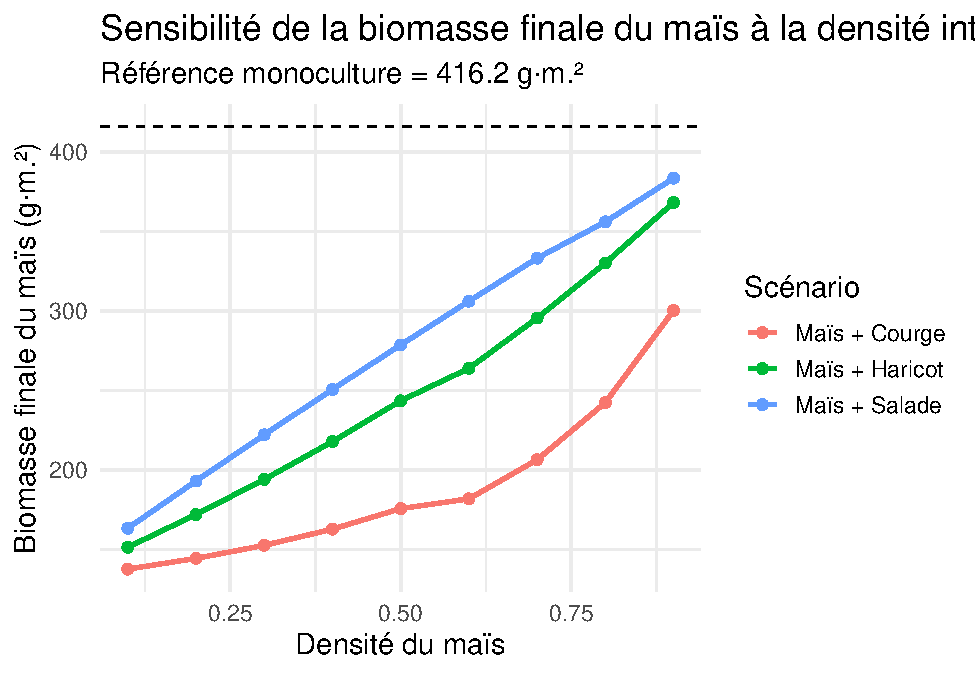
\includegraphics[keepaspectratio]{Rapport_final_Maxime_CORNEZ_files/figure-latex/sensibilité-multiscénarios-1.pdf}}

Une analyse de sensibilité sur l'impact de la densité de culture sur la
production de biomasse du maïs a été effectuée pour chaque scénario
d'interculture. La densité varie de 0,1 à 0,9 par pas de 0,1.

Le graphique issus de l'analyse de sensibilité met en lumière plusieurs
tendances clés quant à l'effet de la densité de maïs sur sa production
finale en interculture :

\begin{itemize}
\item
  \textbf{Progression quasi-linéaire de la biomasse avec la densité\\
  }Pour les trois scénarios d'interculture, la biomasse finale du maïs
  augmente de manière approximativement linéaire lorsque sa densité
  évolue de 0,1 à 0,9. Cette pente positive traduit le fait qu'un
  peuplement plus serré de maïs concentre davantage de surface foliaire
  et de racines par unité de surface, ce qui accroît l'absorption de
  lumière et d'eau --- et donc la fixation de carbone --- jusqu'à 60
  DAS.
\item
  \textbf{Effet de la concurrence par scénario :}

  \begin{itemize}
  \item
    \textbf{Position de la référence monoculture\\
    }La ligne en pointillés (≈416 g·m⁻²) permet de visualiser l'écart
    maximal : aucun scénario interculture n'atteint la production de la
    monoculture, même à densité 0,9. L'écart relatif diminue légèrement
    aux densités élevées, suggérant qu'un maïs très dense compense
    partiellement la compétition, mais sans jamais l'éliminer.
  \item
    \textbf{Maïs + Salade (courbe bleue)\\
    }C'est le scénario où le maïs conserve la production la plus élevée
    à chaque densité : par exemple, à densité 0,5 le maïs produit
    \textasciitilde280 g·m⁻², contre \textasciitilde250 g·m⁻² en haricot
    et \textasciitilde170 g·m⁻² en courge. La salade, à enracinement
    superficiel limité, exerce une concurrence modérée et permet au maïs
    de capter la majeure partie des ressources.
  \item
    \textbf{Maïs + Haricot (courbe verte)\\
    }L'association haricot-maïs se situe en position intermédiaire : la
    biomasse maïs est inférieure d'environ 15 \% à celle obtenue avec
    salade à densité 0,5 (≈240 vs 280 g·m⁻²). Le haricot, grâce à son
    développement racinaire et à une RUE comparable, prélève une part
    non négligeable de l'eau et de la lumière, ce qui se traduit par une
    pente légèrement plus faible que pour le maïs seul.
  \item
    \textbf{Maïs + Courge (courbe rouge)\\
    }La courbe la plus plate : à densité 0,5 le maïs plafonne autour de
    170--180 g·m⁻² (--60 \% par rapport à la monoculture), signe d'une
    forte compétition hydrique et lumineuse exercée par le couvert dense
    de courge. La pente de cette courbe est nettement la plus faible,
    surtout aux faibles densités, ce qui confirme le pouvoir
    concurrentiel de la courge.
  \end{itemize}
\item
  \textbf{Optimisation de la densité :}

  \begin{itemize}
  \item
    \textbf{Faibles densités (\textless{} 0,3)} : la production est très
    réduite pour tous les scénarios, le maïs ne formant pas assez de
    biomasse totale malgré l'absence de concurrence.
  \item
    \textbf{Intermédiaires (0,4--0,6)} : zone de rendement ``optimal''
    en interculture, où la pente reste forte pour salade et haricot,
    mais chute beaucoup pour courge.
  \item
    \textbf{Densités proches de l'équilibre (0,7--0,9)} : les gains
    marginaux de biomasse diminuent, signe d'une saturation des
    ressources (lumière/le sol) et d'effets d'ombrage entre maïs
    eux-mêmes.
  \end{itemize}
\item
  \textbf{Recommandations agronomiques} : pour maximiser la production
  de maïs, privilégier la monoculture ou l'association avec salade à
  densité ≥ 0,6. Pour un système plus équilibré et durable (rendement
  total + services écosystémiques), un compromis autour de densité
  0,5--0,7 en interculture maïs--haricot peut être optimal.
\end{itemize}

\begin{verbatim}
##             Df Sum Sq Mean Sq F value   Pr(>F)    
## Scenario     2  35489   17744   56.96 1.23e-09 ***
## Density      1 103169  103169  331.15 3.75e-15 ***
## Residuals   23   7166     312                     
## ---
## Signif. codes:  0 '***' 0.001 '**' 0.01 '*' 0.05 '.' 0.1 ' ' 1
\end{verbatim}

\begin{verbatim}
## 
##   Simultaneous Tests for General Linear Hypotheses
## 
## Multiple Comparisons of Means: Tukey Contrasts
## 
## 
## Fit: aov(formula = Biomasse_final ~ Scenario + Density, data = sens_stats)
## 
## Linear Hypotheses:
##                                     Estimate Std. Error t value Pr(>|t|)    
## Maïs + Courge - Maïs + Haricot == 0  -59.156      8.321  -7.110  < 0.001 ***
## Maïs + Salade - Maïs + Haricot == 0   27.782      8.321   3.339  0.00763 ** 
## Maïs + Salade - Maïs + Courge == 0    86.938      8.321  10.449  < 0.001 ***
## ---
## Signif. codes:  0 '***' 0.001 '**' 0.01 '*' 0.05 '.' 0.1 ' ' 1
## (Adjusted p values reported -- single-step method)
\end{verbatim}

L'ANOVA à deux facteurs met en évidence que le scénario interculture a
un effet hautement significatif sur la biomasse finale du maïs (F₍₂,₂₃₎
= 56.96, p = 1.23×10⁻⁹) et que la densité joue également un rôle majeur
(F₍₁,₂₃₎ = 331.15, p = 3.75×10⁻¹⁵).

Le test de Tukey post-hoc révèle trois contrastes tous significatifs
après correction :

\begin{itemize}
\item
  Maïs + Courge vs Maïs + Haricot : la production de maïs est en moyenne
  59.2 g·m⁻² inférieure en présence de courge qu'avec haricot (p
  \textless{} 0.001).
\item
  Maïs + Salade vs Maïs + Haricot : le maïs produit 27.8 g·m⁻² de plus
  associé à la salade qu'avec le haricot (p = 0.0078).
\item
  Maïs + Salade vs Maïs + Courge : la salade permet au maïs de gagner
  86.9 g·m⁻² de biomasse de plus que la courge (p \textless{} 0.001).
\end{itemize}

On peut donc classer l'impact des intercultures sur la biomasse du maïs
dans l'ordre décroissant :\\
Salade \textgreater{} Haricot \textgreater{} Courge avec des différences
de l'ordre de 30--90 g·m⁻² selon les associations.

\subsection{Relation entre les racines et la production de
biomasse}\label{relation-entre-les-racines-et-la-production-de-biomasse}

\begin{Shaded}
\begin{Highlighting}[]
\CommentTok{\# 1) Concaténation et mise en long des profondeurs racinaires}
\NormalTok{df\_root\_all }\OtherTok{\textless{}{-}} \FunctionTok{bind\_rows}\NormalTok{(}
\NormalTok{  resultat\_mais          }\SpecialCharTok{\%\textgreater{}\%} \FunctionTok{mutate}\NormalTok{(}\AttributeTok{Scenario =} \StringTok{"Maïs seul"}\NormalTok{)}\SpecialCharTok{\%\textgreater{}\%} \FunctionTok{rename}\NormalTok{(}\AttributeTok{rdepth1 =}\NormalTok{ rdepth),}
\NormalTok{  resultats\_mais\_haricot }\SpecialCharTok{\%\textgreater{}\%} \FunctionTok{mutate}\NormalTok{(}\AttributeTok{Scenario =} \StringTok{"Maïs + Haricot"}\NormalTok{)}\SpecialCharTok{\%\textgreater{}\%} \FunctionTok{rename}\NormalTok{(}\AttributeTok{rdepth1 =}\NormalTok{ rdepth),}
\NormalTok{  resultats\_mais\_courge  }\SpecialCharTok{\%\textgreater{}\%} \FunctionTok{mutate}\NormalTok{(}\AttributeTok{Scenario =} \StringTok{"Maïs + Courge"}\NormalTok{)}\SpecialCharTok{\%\textgreater{}\%} \FunctionTok{rename}\NormalTok{(}\AttributeTok{rdepth1 =}\NormalTok{ rdepth),}
\NormalTok{  resultats\_mais\_salade  }\SpecialCharTok{\%\textgreater{}\%} \FunctionTok{mutate}\NormalTok{(}\AttributeTok{Scenario =} \StringTok{"Maïs + Salade"}\NormalTok{)}\SpecialCharTok{\%\textgreater{}\%} \FunctionTok{rename}\NormalTok{(}\AttributeTok{rdepth1 =}\NormalTok{ rdepth)}
\NormalTok{) }\SpecialCharTok{\%\textgreater{}\%}
  \FunctionTok{pivot\_longer}\NormalTok{(}
    \AttributeTok{cols            =} \FunctionTok{starts\_with}\NormalTok{(}\StringTok{"rdepth"}\NormalTok{),}
    \AttributeTok{names\_to        =} \StringTok{"Culture"}\NormalTok{,}
    \AttributeTok{values\_to       =} \StringTok{"Racine\_mm"}\NormalTok{,}
    \AttributeTok{values\_drop\_na  =} \ConstantTok{TRUE}
\NormalTok{  )}

\CommentTok{\# 2) Tracé en facettes}
\FunctionTok{ggplot}\NormalTok{(df\_root\_all, }\FunctionTok{aes}\NormalTok{(}\AttributeTok{x =}\NormalTok{ Jour, }\AttributeTok{y =}\NormalTok{ Racine\_mm, }\AttributeTok{color =}\NormalTok{ Culture)) }\SpecialCharTok{+}
  \FunctionTok{geom\_line}\NormalTok{(}\AttributeTok{size =} \FloatTok{0.8}\NormalTok{) }\SpecialCharTok{+}
  \FunctionTok{geom\_point}\NormalTok{(}\AttributeTok{size =} \FloatTok{1.5}\NormalTok{) }\SpecialCharTok{+}
  \FunctionTok{facet\_wrap}\NormalTok{(}\SpecialCharTok{\textasciitilde{}}\NormalTok{ Scenario, }\AttributeTok{ncol =} \DecValTok{2}\NormalTok{) }\SpecialCharTok{+}
  \FunctionTok{labs}\NormalTok{(}
    \AttributeTok{title =} \StringTok{"Évolution de la profondeur racinaire"}\NormalTok{,}
    \AttributeTok{x     =} \StringTok{"DAS"}\NormalTok{,}
    \AttributeTok{y     =} \StringTok{"Profondeur racinaire [mm]"}\NormalTok{,}
    \AttributeTok{color =} \StringTok{"Culture"}
\NormalTok{  ) }\SpecialCharTok{+}
  \FunctionTok{theme\_minimal}\NormalTok{(}\AttributeTok{base\_size =} \DecValTok{14}\NormalTok{) }\SpecialCharTok{+}
  \FunctionTok{theme}\NormalTok{(}\AttributeTok{strip.text =} \FunctionTok{element\_text}\NormalTok{(}\AttributeTok{face =} \StringTok{"bold"}\NormalTok{))}
\end{Highlighting}
\end{Shaded}

\begin{center}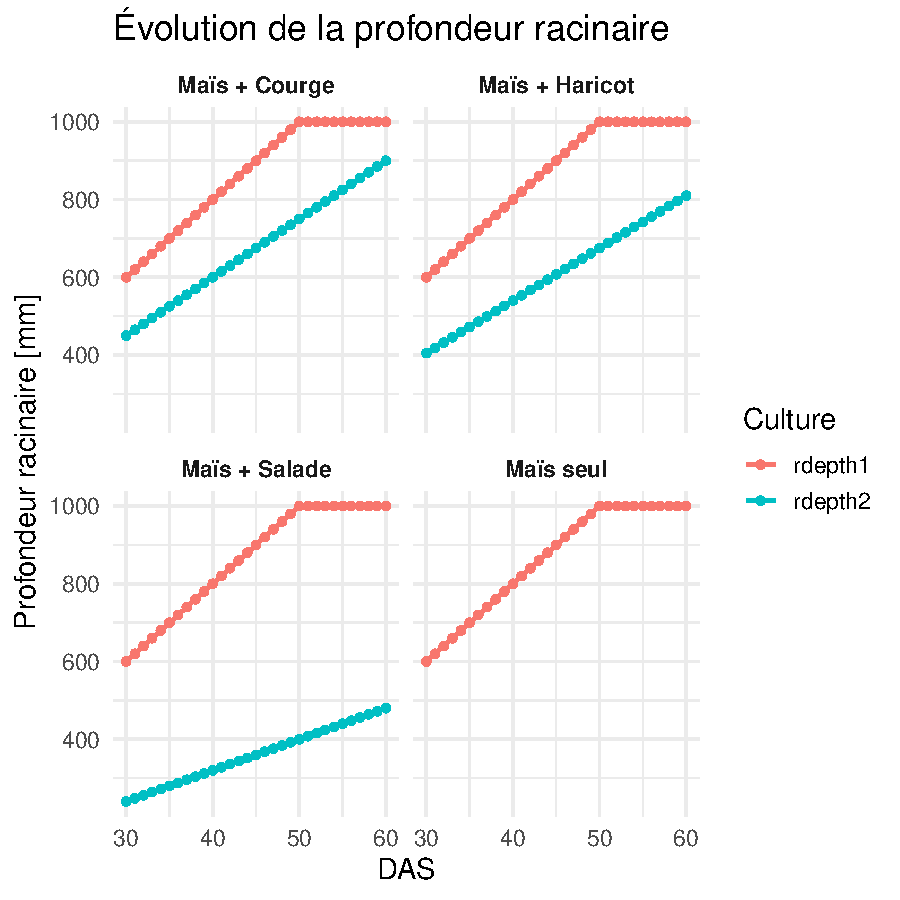
\includegraphics[width=0.7\linewidth]{Rapport_final_Maxime_CORNEZ_files/figure-latex/graphe-rdepth-1} \end{center}

Dans ce modèle minimaliste, la dynamique de développement racinaire
n'est pas affectée par la présence d'une seconde espèce : chaque culture
voit sa racine progresser linéairement jusqu'à une profondeur maximale
(≈ 1 000 mm) définie a priori, indépendamment de la compétition
interculture. En réalité, on observe que :

\begin{itemize}
\item
  \textbf{Le maïs} (courbe rouge) atteint la profondeur maximale la plus
  élevée et rapidement (vers 50 DAS),
\item
  \textbf{La courge} (courbe bleue, haut-gauche) suit avec un
  enracinement proche mais légèrement retardé,
\item
  \textbf{Le haricot} (courbe bleue, haut-droite) affiche une
  progression similaire à celle de la courge,
\item
  \textbf{La salade} (courbe bleue, bas-gauche) reste nettement plus
  superficielle, plafonnant autour de 500 mm à 60 DAS.
\end{itemize}

Cette uniformité de la croissance racinaire à la monoculture et à
l'interculture résulte de l'absence, dans le modèle, de feedbacks liant
compétition pour l'eau et extension racinaire. Pourtant, c'est
précisément ce potentiel de profondeur qui dicte la capacité
d'exploration des horizons les plus profonds et, par conséquent, l'accès
à l'eau stockée dans le sol : la salade, dont le système racinaire reste
très peu développé, ne peut pas puiser dans les réserves profondes et
dépend presque exclusivement des premières dizaines de centimètres de
terrain, tandis que maïs, courge et haricot bénéficient de l'apport
hydrique plus stable des couches plus basses.

Il serait grandement profitable de lier le modèle APSIM à un modèle de
modélisation racinaire comme CRootBox afin de mieux developper le
feedback entre la production racinaire et la quantité d'eau disponible.

\begin{Shaded}
\begin{Highlighting}[]
\CommentTok{\# 1) Concaténer les données racines vs biomasse journalière}
\NormalTok{df\_root\_biom }\OtherTok{\textless{}{-}} \FunctionTok{bind\_rows}\NormalTok{(}
\NormalTok{  resultat\_mais }\SpecialCharTok{\%\textgreater{}\%}
    \FunctionTok{transmute}\NormalTok{(}
      \AttributeTok{Scenario  =} \StringTok{"Maïs seul"}\NormalTok{,}
      \AttributeTok{rdepth    =}\NormalTok{ rdepth,}
      \AttributeTok{biomasse  =}\NormalTok{ Biomasse\_reelle}
\NormalTok{    ),}
\NormalTok{  resultats\_mais\_haricot }\SpecialCharTok{\%\textgreater{}\%}
    \FunctionTok{transmute}\NormalTok{(}\AttributeTok{Scenario =} \StringTok{"Maïs + Haricot"}\NormalTok{, }\AttributeTok{rdepth =}\NormalTok{ rdepth,     }\AttributeTok{biomasse =}\NormalTok{ Biomasse1),}
\NormalTok{  resultats\_mais\_courge  }\SpecialCharTok{\%\textgreater{}\%}
    \FunctionTok{transmute}\NormalTok{(}\AttributeTok{Scenario =} \StringTok{"Maïs + Courge"}\NormalTok{,  }\AttributeTok{rdepth =}\NormalTok{ rdepth,     }\AttributeTok{biomasse =}\NormalTok{ Biomasse1),}
\NormalTok{  resultats\_mais\_salade  }\SpecialCharTok{\%\textgreater{}\%}
    \FunctionTok{transmute}\NormalTok{(}\AttributeTok{Scenario =} \StringTok{"Maïs + Salade"}\NormalTok{,  }\AttributeTok{rdepth =}\NormalTok{ rdepth,     }\AttributeTok{biomasse =}\NormalTok{ Biomasse1)}
\NormalTok{)}

\CommentTok{\# 2) Test de corrélation de Pearson}
\NormalTok{cor\_test }\OtherTok{\textless{}{-}} \FunctionTok{cor.test}\NormalTok{(df\_root\_biom}\SpecialCharTok{$}\NormalTok{rdepth, df\_root\_biom}\SpecialCharTok{$}\NormalTok{biomasse)}
\NormalTok{r\_val   }\OtherTok{\textless{}{-}} \FunctionTok{round}\NormalTok{(cor\_test}\SpecialCharTok{$}\NormalTok{estimate, }\DecValTok{2}\NormalTok{)}
\NormalTok{p\_val   }\OtherTok{\textless{}{-}} \FunctionTok{signif}\NormalTok{(cor\_test}\SpecialCharTok{$}\NormalTok{p.value, }\DecValTok{2}\NormalTok{)}
\NormalTok{corr\_label }\OtherTok{\textless{}{-}} \FunctionTok{paste0}\NormalTok{(}\StringTok{"r = "}\NormalTok{, r\_val, }\StringTok{"}\SpecialCharTok{\textbackslash{}n}\StringTok{"}\NormalTok{, }\StringTok{"p = "}\NormalTok{, p\_val)}

\CommentTok{\# 3) Nuage de points + droite de régression + annotation}
\FunctionTok{ggplot}\NormalTok{(df\_root\_biom, }\FunctionTok{aes}\NormalTok{(}\AttributeTok{x =}\NormalTok{ rdepth, }\AttributeTok{y =}\NormalTok{ biomasse, }\AttributeTok{color =}\NormalTok{ Scenario)) }\SpecialCharTok{+}
  \FunctionTok{geom\_point}\NormalTok{(}\AttributeTok{alpha =} \FloatTok{0.7}\NormalTok{) }\SpecialCharTok{+}
  \FunctionTok{geom\_smooth}\NormalTok{(}\AttributeTok{method =} \StringTok{"lm"}\NormalTok{, }\AttributeTok{se =} \ConstantTok{FALSE}\NormalTok{) }\SpecialCharTok{+}
  \FunctionTok{annotate}\NormalTok{(}
    \StringTok{"text"}\NormalTok{,}
    \AttributeTok{x =} \ConstantTok{Inf}\NormalTok{, }\AttributeTok{y =} \ConstantTok{Inf}\NormalTok{,}
    \AttributeTok{label =}\NormalTok{ corr\_label,}
    \AttributeTok{hjust =} \FloatTok{1.1}\NormalTok{, }\AttributeTok{vjust =} \FloatTok{1.5}\NormalTok{,}
    \AttributeTok{size =} \DecValTok{4}\NormalTok{,}
    \AttributeTok{color =} \StringTok{"black"}
\NormalTok{  ) }\SpecialCharTok{+}
  \FunctionTok{labs}\NormalTok{(}
    \AttributeTok{title =} \StringTok{"Relation profondeur racinaire vs biomasse journalière"}\NormalTok{,}
    \AttributeTok{x     =} \StringTok{"Profondeur racinaire (mm)"}\NormalTok{,}
    \AttributeTok{y     =} \StringTok{"Biomasse journalière (g·m⁻²)"}
\NormalTok{  ) }\SpecialCharTok{+}
  \FunctionTok{theme\_minimal}\NormalTok{(}\AttributeTok{base\_size =} \DecValTok{14}\NormalTok{)}
\end{Highlighting}
\end{Shaded}

\pandocbounded{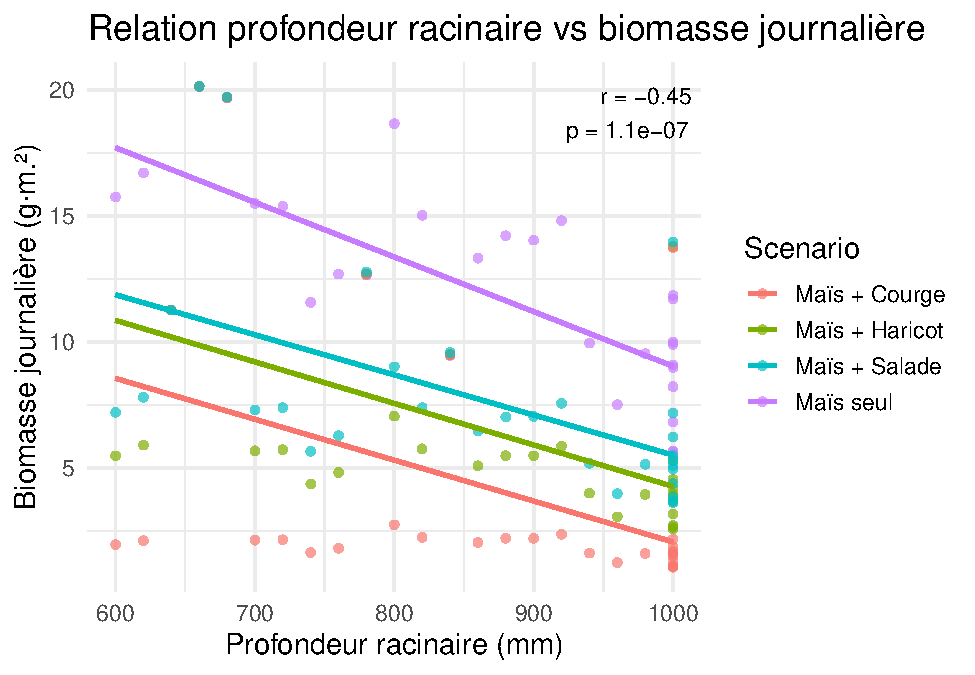
\includegraphics[keepaspectratio]{Rapport_final_Maxime_CORNEZ_files/figure-latex/couplage-racines-biomasse-1.pdf}}

\begin{Shaded}
\begin{Highlighting}[]
\CommentTok{\# 1) Préparer la liste des modèles}
\NormalTok{models }\OtherTok{\textless{}{-}} \FunctionTok{list}\NormalTok{(}
  \StringTok{"Maïs seul"}       \OtherTok{=} \FunctionTok{lm}\NormalTok{(Biomasse\_reelle              }\SpecialCharTok{\textasciitilde{}}\NormalTok{ rdepth,             }\AttributeTok{data =}\NormalTok{ resultat\_mais),}
  \StringTok{"Maïs + Haricot"}  \OtherTok{=} \FunctionTok{lm}\NormalTok{((Biomasse1 }\SpecialCharTok{+}\NormalTok{ Biomasse2)     }\SpecialCharTok{\textasciitilde{}}\NormalTok{ rdepth }\SpecialCharTok{+}\NormalTok{ rdepth2,   }\AttributeTok{data =}\NormalTok{ resultats\_mais\_haricot),}
  \StringTok{"Maïs + Courge"}   \OtherTok{=} \FunctionTok{lm}\NormalTok{((Biomasse1 }\SpecialCharTok{+}\NormalTok{ Biomasse2)     }\SpecialCharTok{\textasciitilde{}}\NormalTok{ rdepth }\SpecialCharTok{+}\NormalTok{ rdepth2,   }\AttributeTok{data =}\NormalTok{ resultats\_mais\_courge),}
  \StringTok{"Maïs + Salade"}   \OtherTok{=} \FunctionTok{lm}\NormalTok{((Biomasse1 }\SpecialCharTok{+}\NormalTok{ Biomasse2)     }\SpecialCharTok{\textasciitilde{}}\NormalTok{ rdepth }\SpecialCharTok{+}\NormalTok{ rdepth2,   }\AttributeTok{data =}\NormalTok{ resultats\_mais\_salade)}
\NormalTok{)}

\CommentTok{\# 2) Extraire coefficients et statistics de chaque modèle}
\NormalTok{reg\_coefs }\OtherTok{\textless{}{-}} 
  \FunctionTok{imap\_dfr}\NormalTok{(models, }\SpecialCharTok{\textasciitilde{}} \FunctionTok{tidy}\NormalTok{(.x) }\SpecialCharTok{\%\textgreater{}\%} 
             \FunctionTok{filter}\NormalTok{(term }\SpecialCharTok{!=} \StringTok{"(Intercept)"}\NormalTok{) }\SpecialCharTok{\%\textgreater{}\%} 
\NormalTok{             dplyr}\SpecialCharTok{::}\FunctionTok{select}\NormalTok{(term, estimate, std.error, p.value) }\SpecialCharTok{\%\textgreater{}\%} 
             \FunctionTok{mutate}\NormalTok{(}\AttributeTok{Scenario =}\NormalTok{ .y),}
           \AttributeTok{.id =} \ConstantTok{NULL}\NormalTok{)}

\CommentTok{\# 3) Extraire R² ajusté et p{-}value globale}
\NormalTok{reg\_glance }\OtherTok{\textless{}{-}} 
  \FunctionTok{imap\_dfr}\NormalTok{(models, }\SpecialCharTok{\textasciitilde{}} \FunctionTok{glance}\NormalTok{(.x) }\SpecialCharTok{\%\textgreater{}\%} 
\NormalTok{             dplyr}\SpecialCharTok{::}\FunctionTok{select}\NormalTok{(r.squared, adj.r.squared, p.value) }\SpecialCharTok{\%\textgreater{}\%} 
             \FunctionTok{mutate}\NormalTok{(}\AttributeTok{Scenario =}\NormalTok{ .y),}
           \AttributeTok{.id =} \ConstantTok{NULL}\NormalTok{)}

\CommentTok{\# 4) Combiner en un seul tableau}
\NormalTok{reg\_summary }\OtherTok{\textless{}{-}} 
  \FunctionTok{left\_join}\NormalTok{(reg\_coefs, reg\_glance, }\AttributeTok{by =} \StringTok{"Scenario"}\NormalTok{) }\SpecialCharTok{\%\textgreater{}\%}
\NormalTok{  dplyr}\SpecialCharTok{::}\FunctionTok{select}\NormalTok{(}
\NormalTok{    Scenario, term, }
    \AttributeTok{slope           =}\NormalTok{ estimate,}
    \StringTok{\textasciigrave{}}\AttributeTok{Std. Error}\StringTok{\textasciigrave{}}    \OtherTok{=}\NormalTok{ std.error,}
    \StringTok{\textasciigrave{}}\AttributeTok{p{-}value slope}\StringTok{\textasciigrave{}} \OtherTok{=}\NormalTok{ p.value.x,}
    \StringTok{\textasciigrave{}}\AttributeTok{R²}\StringTok{\textasciigrave{}}            \OtherTok{=}\NormalTok{ r.squared,}
    \StringTok{\textasciigrave{}}\AttributeTok{R² ajusté}\StringTok{\textasciigrave{}}     \OtherTok{=}\NormalTok{ adj.r.squared,}
    \StringTok{\textasciigrave{}}\AttributeTok{p{-}value global}\StringTok{\textasciigrave{}}\OtherTok{=}\NormalTok{ p.value.y}
\NormalTok{  )}

\CommentTok{\# 5) Afficher}
\NormalTok{knitr}\SpecialCharTok{::}\FunctionTok{kable}\NormalTok{(}
\NormalTok{  reg\_summary,}
  \AttributeTok{caption =} \StringTok{"Synthèse des régressions linéaires par scénario"}
\NormalTok{)}
\end{Highlighting}
\end{Shaded}

\begin{longtable}[]{@{}
  >{\raggedright\arraybackslash}p{(\linewidth - 14\tabcolsep) * \real{0.1596}}
  >{\raggedright\arraybackslash}p{(\linewidth - 14\tabcolsep) * \real{0.0851}}
  >{\raggedleft\arraybackslash}p{(\linewidth - 14\tabcolsep) * \real{0.1170}}
  >{\raggedleft\arraybackslash}p{(\linewidth - 14\tabcolsep) * \real{0.1170}}
  >{\raggedleft\arraybackslash}p{(\linewidth - 14\tabcolsep) * \real{0.1489}}
  >{\raggedleft\arraybackslash}p{(\linewidth - 14\tabcolsep) * \real{0.1064}}
  >{\raggedleft\arraybackslash}p{(\linewidth - 14\tabcolsep) * \real{0.1064}}
  >{\raggedleft\arraybackslash}p{(\linewidth - 14\tabcolsep) * \real{0.1596}}@{}}
\caption{Synthèse des régressions linéaires par scénario}\tabularnewline
\toprule\noalign{}
\begin{minipage}[b]{\linewidth}\raggedright
Scenario
\end{minipage} & \begin{minipage}[b]{\linewidth}\raggedright
term
\end{minipage} & \begin{minipage}[b]{\linewidth}\raggedleft
slope
\end{minipage} & \begin{minipage}[b]{\linewidth}\raggedleft
Std. Error
\end{minipage} & \begin{minipage}[b]{\linewidth}\raggedleft
p-value slope
\end{minipage} & \begin{minipage}[b]{\linewidth}\raggedleft
R²
\end{minipage} & \begin{minipage}[b]{\linewidth}\raggedleft
R² ajusté
\end{minipage} & \begin{minipage}[b]{\linewidth}\raggedleft
p-value global
\end{minipage} \\
\midrule\noalign{}
\endfirsthead
\toprule\noalign{}
\begin{minipage}[b]{\linewidth}\raggedright
Scenario
\end{minipage} & \begin{minipage}[b]{\linewidth}\raggedright
term
\end{minipage} & \begin{minipage}[b]{\linewidth}\raggedleft
slope
\end{minipage} & \begin{minipage}[b]{\linewidth}\raggedleft
Std. Error
\end{minipage} & \begin{minipage}[b]{\linewidth}\raggedleft
p-value slope
\end{minipage} & \begin{minipage}[b]{\linewidth}\raggedleft
R²
\end{minipage} & \begin{minipage}[b]{\linewidth}\raggedleft
R² ajusté
\end{minipage} & \begin{minipage}[b]{\linewidth}\raggedleft
p-value global
\end{minipage} \\
\midrule\noalign{}
\endhead
\bottomrule\noalign{}
\endlastfoot
Maïs seul & rdepth & -0.0217042 & 0.0035793 & 0.0000013 & 0.5590641 &
0.5438594 & 0.0000013 \\
Maïs + Haricot & rdepth & -0.0108070 & 0.0218842 & 0.6252806 & 0.3674232
& 0.3222392 & 0.0016428 \\
Maïs + Haricot & rdepth2 & -0.0157989 & 0.0247684 & 0.5287444 &
0.3674232 & 0.3222392 & 0.0016428 \\
Maïs + Courge & rdepth & -0.0155261 & 0.0266741 & 0.5651794 & 0.2502924
& 0.1967419 & 0.0177209 \\
Maïs + Courge & rdepth2 & -0.0074706 & 0.0271706 & 0.7853721 & 0.2502924
& 0.1967419 & 0.0177209 \\
Maïs + Salade & rdepth & -0.0069045 & 0.0178072 & 0.7011426 & 0.3416076
& 0.2945796 & 0.0028760 \\
Maïs + Salade & rdepth2 & -0.0231687 & 0.0340101 & 0.5013215 & 0.3416076
& 0.2945796 & 0.0028760 \\
\end{longtable}

Dans toutes les situations, on observe une pente négative de la relation
entre profondeur racinaire et production journalière de biomasse : plus
les racines s'allongent, moins la plante produit de biomasse chaque
jour. Cette « corrélation » n'est pas un effet causal direct, mais
traduit simplement que, dans notre modèle, l'augmentation linéaire de la
profondeur racinaire survient en fin de cycle, alors que la croissance
foliaire tend naturellement à ralentir.

\begin{itemize}
\item
  \textbf{Maïs seul} : la régression donne une pente de --0,0217
  g·m⁻²·mm⁻¹ (p \textless{} 10⁻⁶, R²ajusté = 0,54). Autrement dit, pour
  chaque millimètre de racine supplémentaire, la biomasse journalière
  diminue de \textasciitilde0,02 g·m⁻², ce qui reflète plutot le déclin
  de la croissance vers la fin de la simulation.
\item
  \textbf{Maïs + Haricot} : pente maïs --0,0108 (p = 0,63, R²ajusté =
  0,32) et pente haricot --0,0160 (p = 0,53). La relation est encore
  négative mais non significative, montrant que la compétition hydrique
  et lumineuse entre deux espèces efface l'effet temporel simple observé
  en monoculture.
\item
  \textbf{Maïs + Courge} : pente maïs --0,0155 (p = 0,57, R²ajusté =
  0,20) et pente courge --0,0075 (p = 0,79). Même constat : l'extension
  racinaire ne suffit plus à expliquer la production quotidienne de
  biomasse.
\item
  \textbf{Maïs + Salade} : pente maïs --0,0069 (p = 0,70, R²ajusté =
  0,29) et pente salade --0,0232 (p = 0,50). La courbe salade, aux
  racines peu profondes, montre un léger déclin quotidien, mais là
  encore non significatif.
\end{itemize}

En conclusion, dans ce cadre purement « racine linéaire → eau → biomasse
», la profondeur n'est qu'un proxy du temps et ne pilote pas directement
la production journalière. Seule la monoculture révèle une relation
significative (pente et R² élevées).

\newpage

\section{Conclusion}\label{conclusion}

Dans cette étude, nous avons prolongé le cadre classique d'APSIM
monoculture pour développer un modèle duo capable de simuler la
co-culture de deux espèces (maïs + plante associée) sur un profil de sol
à trois horizons, en intégrant la compétition hydrique via un arbitrage
de la transpiration. La transition du modèle mono au modèle duo s'appuie
sur trois étapes clés :

\begin{enumerate}
\def\labelenumi{\arabic{enumi}.}
\item
  \textbf{Reproduction du module monoculture} : nous avons d'abord
  implémenté et validé le simulateur mono-culture (maïs seul), en
  vérifiant que, pour chaque jour, la transpiration réelle ne dépasse
  jamais l'offre potentielle en eau du sol (Pot\_Supply ≥
  Transpiration), garantissant la cohérence physique des calculs et la
  stabilité numérique.
\item
  \textbf{Extension au duo-culture} : chaque espèce conserve sa propre
  dynamique racinaire (croissance linéaire avec VPR), sa demande
  hydrique (liée au LAI et à la radiation) et sa production organique,
  mais la distribution journalière de l'eau est partagée
  proportionnellement aux demandes relatives. Cette approche simple mais
  robuste préserve l'intégrité des mécanismes fondamentaux (extraction,
  transpiration, biomasse) tout en autorisant des scénarios
  d'association variés.
\item
  \textbf{Vérifications de sensibilité et de plausibilité} :

  \begin{itemize}
  \item
    \textbf{Transpiration} ne depasse pas l'offre, la validation des
    simulations a montré que, quel que soit le scénario, l'offre en eau
    du sol (Pot\_Supply) reste systématiquement supérieure à la demande
    réelle de transpiration, garantissant la cohérence physique du
    modèle.
  \item
    \textbf{Réserves en eau} : l'analyse des stocks restants à J60
    révèle qu'en interculture, chaque scénario retient davantage d'eau
    profonde (jusqu'à +10 mm dans l'horizon 3 vs monoculture),
    confirmant une exploitation plus équilibrée du profil.\\
    Le maïs exploite profondément le profil (horizon 3 laissé à
    seulement \textasciitilde11 mm à J60), alors qu'en interculture
    l'eau profonde est mieux préservée (jusqu'à \textasciitilde20 mm
    résiduels), signe d'une répartition racinaire plus complémentaire ou
    d'une moindre demande globale.
  \item
    \textbf{Ratio Offre/Demande (O/D)} : le nombre de jours de stress
    hydrique (O/D \textless{} 1) passe de 26 en mono à 31 en
    interculture, soulignant un léger accroissement des épisodes de
    tension, mais laissé à un niveau acceptable pour la période simulée
    (30 jours).
  \item
    \textbf{Production de biomasse} :

    \begin{itemize}
    \item
      \emph{Monoculture :} le maïs atteint 416 g·m⁻² à J60 (pente = 12
      g·m⁻²·j⁻¹).
    \item
      \emph{Maïs + Courge :} 176 g·m⁻² pour le maïs (--58 \%), 126 g·m⁻²
      pour la courge,
    \item
      \emph{Maïs + Haricot :} 244 g·m⁻² pour le maïs (--41 \%), 124
      g·m⁻² pour le haricot,
    \item
      \emph{Maïs + Salade :} 279 g·m⁻² pour le maïs (--33 \%), 49 g·m⁻²
      pour la salade.
    \end{itemize}
  \end{itemize}

  Ces résultats montrent que chaque plante associée capte un volume
  d'eau et de lumière capable de réduire significativement la croissance
  du maïs, illustrant le compromis classique entre rendement de la
  culture principale et valeur ajoutée de la culture secondaire.
\item
  \textbf{Analyse de sensibilité :} en faisant varier la densité
  relative du maïs (0,1 à 0,9) dans les intercultures, nous avons
  observé une décroissance quasi‐linéaire de la biomasse finale du maïs
  à J60 en présence d'une interculture. Chaque espèce associée affichant
  une pente caractéristique : la salade réduit le moins la production
  (pente modérée), tandis que la courge et le haricot exercent une
  pression plus forte. La valeur de référence en monoculture (416 g·m⁻²)
  a été tracée pour visualiser la perte/addition relative. Un test ANOVA
  a confirmé que la densité (p \textless{} 10⁻¹⁴) et le scénario
  interculture (p \textless{} 10⁻⁹) influencent significativement la
  biomasse du maïs, et un test de Tukey a montré des différences
  marquées entre chaque couple de scénarios (toutes p \textless{} 0,01).
\item
  \textbf{Perspectives :} plusieurs axes d'enrichissement du modèle
  méritent d'être explorés :

  \begin{enumerate}
  \def\labelenumii{\arabic{enumii}.}
  \item
    \textbf{Compétition lumineuse} : coupler l'interaction des LAI pour
    mieux simuler l'ombrage mutuel et les effets de concurrence
    foliaire.
  \item
    \textbf{Dynamique azotée} : introduire le module N d'APSIM pour
    quantifier l'apport fertilisant des légumineuses (fixation
    symbiotique) et ses retombées sur la croissance du maïs.
  \item
    \textbf{Plasticité racinaire} : substituer la croissance linéaire
    par une répartition adaptative des racines, modulée par l'humidité
    locale des horizons et la densité de peuplement.
  \item
    \textbf{Validation terrain} : confronter les simulations à des jeux
    de données expérimentales (flux de transpiration, mesures de
    biomasse, observations racinaires), afin d'ajuster et calibrer les
    coefficients d'extraction (kl), d'expansion foliaire (CEF) et de
    conversion (RUE, TEC).
  \end{enumerate}
\end{enumerate}

En somme, le passage du modèle mono au modèle duo, validé par des tests
de cohérence hydrique et agronomique, offre un outil versatile pour
étudier les compromis agro‐écologiques en interculture. Il permet
d'informer la conduite de cultures associées, que ce soit pour maximiser
la production de maïs (monoculture ou intercalée avec salade) ou pour
équilibrer les rendements de systèmes maïs--légumineuse (haricot,
courge), tout en préparant le terrain pour intégrer d'autres services
écosystémiques (fertilité, biodiversité).

\newpage

\section{Collaboration}\label{collaboration}

Lors de ce projet j'ai eu l'occasion de collaborer avec plusieurs
collègues autant pour améliorer mon projet que pour les aider avec le
leur.

Je tiens à remercier tout particulièrement Alice Falzon avec qui j'ai
travaillé à l'élaboration du modèle APSIM\_2025, qui est la base de ce
projet, elle m'a aussi fourni le code pour obtenir les données météo
réelles via Open-Meteo et pour ses retours concernant mon rapport.\\
En retour j'ai pu l'aider à améliorer quelques points de son modèle et
j'ai aussi relu son rapport.

Nous avons partagé notre code avec le reste de la classe, mais je ne
saurais dire précisément qui l'a utilisé.

Je remercie aussi Ismael Peeters pour son aide sur la théorie lié au kl.

J'ai pu aider Emile Davio et Zoé Saintrain sur des points relatifs à la
théorie et au code d'APSIM.

\newpage

\section*{Références}\label{ruxe9fuxe9rences}
\addcontentsline{toc}{section}{Références}

\phantomsection\label{refs}
\begin{CSLReferences}{1}{0}
\bibitem[\citeproctext]{ref-open-meteo_2025}
{``🌤️ {Free} {Open}-{Source} {Weather} {API} {\textbar}
{Open}-{Meteo}.com.''} 2025. \url{https://open-meteo.com/}.

\bibitem[\citeproctext]{ref-barnabas_effect_2008}
Barnabás, Beáta, Katalin Jäger, and Attila Fehér. 2008. {``The Effect of
Drought and Heat Stress on Reproductive Processes in Cereals.''}
\emph{Plant, Cell \& Environment} 31 (1): 11--38.
\url{https://doi.org/10.1111/j.1365-3040.2007.01727.x}.

\bibitem[\citeproctext]{ref-bondeau_modelling_2007}
Bondeau, Alberte, Pascalle C. Smith, Sönke Zaehle, Sibyll Schaphoff,
Wolfgang Lucht, Wolfgang Cramer, Dieter Gerten, et al. 2007.
{``Modelling the Role of Agriculture for the 20th Century Global
Terrestrial Carbon Balance.''} \emph{Global Change Biology} 13 (3):
679--706. \url{https://doi.org/10.1111/j.1365-2486.2006.01305.x}.

\bibitem[\citeproctext]{ref-brennan_agronomic_2013}
Brennan, Eric B. 2013. {``Agronomic Aspects of Strip Intercropping
Lettuce with Alyssum for Biological Control of Aphids.''}
\emph{Biological Control} 65 (3): 302--11.
https://doi.org/\url{https://doi.org/10.1016/j.biocontrol.2013.03.017}.

\bibitem[\citeproctext]{ref-brooker_improving_2015}
Brooker, Rob W., Alison E. Bennett, Wen-Feng Cong, Tim J. Daniell,
Timothy S. George, Paul D. Hallett, Cathy Hawes, et al. 2015.
{``Improving Intercropping: A Synthesis of Research in Agronomy, Plant
Physiology and Ecology.''} \emph{New Phytologist} 206 (1): 107--17.
\url{https://doi.org/10.1111/nph.13132}.

\bibitem[\citeproctext]{ref-cryan_yield_2025}
Cryan, Ty, Olivia Musselman, Aaron W. Baumgardner, Sadie Osborn,
Caroline J. Beuscher, Caitlin Stehn, Ariane Burt, et al. 2025. {``Yield,
Growth, and Labor Demands of Growing Maize, Beans, and Squash in
Monoculture Versus the {Three} {Sisters}.''} \emph{PLANTS, PEOPLE,
PLANET} 7 (1): 204--14. \url{https://doi.org/10.1002/ppp3.10576}.

\bibitem[\citeproctext]{ref-dong_maize_2022}
Dong, Qiqi, Xinhua Zhao, Dongying Zhou, Zhenhua Liu, Xiaolong Shi, Yang
Yuan, Peiyan Jia, et al. 2022. {``Maize and Peanut Intercropping
Improves the Nitrogen Accumulation and Yield Per Plant of Maize by
Promoting the Secretion of Flavonoids and Abundance of {Bradyrhizobium}
in Rhizosphere.''} \emph{Frontiers in Plant Science} 13 (August).
\url{https://doi.org/10.3389/fpls.2022.957336}.

\bibitem[\citeproctext]{ref-draye_practical}
Draye, Xavier. n.d. {``Practical Notes.''}

\bibitem[\citeproctext]{ref-dudgeon_freshwater_2006}
Dudgeon, David, Angela H. Arthington, Mark O. Gessner, Zen-Ichiro
Kawabata, Duncan J. Knowler, Christian Lévêque, Robert J. Naiman, et al.
2006. {``Freshwater Biodiversity: Importance, Threats, Status and
Conservation Challenges.''} \emph{Biological Reviews} 81 (2): 163--82.
\url{https://doi.org/10.1017/S1464793105006950}.

\bibitem[\citeproctext]{ref-foley_global_2005}
Foley, Jonathan A., Ruth DeFries, Gregory P. Asner, Carol Barford,
Gordon Bonan, Stephen R. Carpenter, F. Stuart Chapin, et al. 2005.
{``Global {Consequences} of {Land} {Use}.''} \emph{Science} 309 (5734):
570--74. \url{https://doi.org/10.1126/science.1111772}.

\bibitem[\citeproctext]{ref-ghavidel_evaluation_2016}
Ghavidel, Raheleh, Ghorban Asadi, Mohammad Naseri, Pour Yazdi, Reza
Ghorbani, and Surur Khorramdel. 2016. {``Evaluation of Radiation Use
Efficiency of Common Bean ({Phaseolus} Vulgaris {L}.) Cultivars as
Affected by Plant Density Under {Mashhad} Climatic Conditions.''}
\emph{J. BioSci. Biotechnol.} 5 (2): 145--50.

\bibitem[\citeproctext]{ref-hammer_computer_2009}
Hammer, G. 2009. {``Computer Session: Yield Prediction, Simulation of
the Genotype {X} Environment Interaction with an {Excel} Version of
{APSIM}.''}

\bibitem[\citeproctext]{ref-keating_overview_2003}
Keating, B. A, P. S Carberry, G. L Hammer, M. E Probert, M. J Robertson,
D Holzworth, N. I Huth, et al. 2003. {``An Overview of {APSIM}, a Model
Designed for Farming Systems Simulation.''} \emph{European Journal of
Agronomy}, Modelling {Cropping} {Systems}: {Science}, {Software} and
{Applications}, 18 (3): 267--88.
\url{https://doi.org/10.1016/S1161-0301(02)00108-9}.

\bibitem[\citeproctext]{ref-lin_effects_2013}
Lin, Kuan-Hung, Meng-Yuan Huang, Wen-Dar Huang, Ming-Huang Hsu, Zhi-Wei
Yang, and Chi-Ming Yang. 2013. {``The Effects of Red, Blue, and White
Light-Emitting Diodes on the Growth, Development, and Edible Quality of
Hydroponically Grown Lettuce (\emph{{Lactuca} Sativa} {L}. Var.
\emph{Capitata}).''} \emph{Scientia Horticulturae} 150 (February):
86--91. \url{https://doi.org/10.1016/j.scienta.2012.10.002}.

\bibitem[\citeproctext]{ref-mccown_apsim_1996}
McCown, R. L., G. L. Hammer, J. N. G. Hargreaves, D. P. Holzworth, and
D. M. Freebairn. 1996. {``{APSIM}: A Novel Software System for Model
Development, Model Testing and Simulation in Agricultural Systems
Research.''} \emph{Agricultural Systems} 50 (3): 255--71.
\url{https://doi.org/10.1016/0308-521X(94)00055-V}.

\bibitem[\citeproctext]{ref-mudare_yield_2022}
Mudare, Shingirai, Jasper Kanomanyanga, Xiaoqiang Jiao, Stanford Mabasa,
Jay Ram Lamichhane, Jingying Jing, and Wen-Feng Cong. 2022. {``Yield and
Fertilizer Benefits of Maize/Grain Legume Intercropping in {China} and
{Africa}: {A} Meta-Analysis.''} \emph{Agronomy for Sustainable
Development} 42 (5): 81.
\url{https://doi.org/10.1007/s13593-022-00816-1}.

\bibitem[\citeproctext]{ref-munns_comparative_2002}
Munns, R. 2002. {``Comparative Physiology of Salt and Water Stress.''}
\emph{Plant, Cell \& Environment} 25 (2): 239--50.
https://doi.org/\url{https://doi.org/10.1046/j.0016-8025.2001.00808.x}.

\bibitem[\citeproctext]{ref-nassary_productivity_2020}
Nassary, Eliakira Kisetu, Frederick Baijukya, and Patrick Alois
Ndakidemi. 2020. {``Productivity of Intercropping with Maize and Common
Bean over Five Cropping Seasons on Smallholder Farms of {Tanzania}.''}
\emph{European Journal of Agronomy} 113 (February): 125964.
\url{https://doi.org/10.1016/j.eja.2019.125964}.

\bibitem[\citeproctext]{ref-ogindo_determination_2004}
Ogindo, H. O., and S. Walker. 2004. {``The Determination of
Transpiration Efficiency Coefficient for Common Bean.''} \emph{Physics
and Chemistry of the Earth, Parts A/B/C}, Water, {Science}, {Technology}
and {Policy} {Convergence} and {Action} by {All} ({A} {Meeting} {Point}
for {Action} leading to {Sustainable} {Development}), 29 (15): 1083--89.
\url{https://doi.org/10.1016/j.pce.2004.09.025}.

\bibitem[\citeproctext]{ref-rouphael_radiation_2005}
Rouphael, Youssef, and Giuseppe Colla. 2005. {``Radiation and Water Use
Efficiencies of Greenhouse Zucchini Squash in Relation to Different
Climate Parameters.''} \emph{European Journal of Agronomy} 23 (2):
183--94. \url{https://doi.org/10.1016/j.eja.2004.10.003}.

\bibitem[\citeproctext]{ref-tremblay_comparison_2004}
Tremblay, Marie, and Daniel Wallach. 2004. {``Comparison of Parameter
Estimation Methods for Crop Models.''} \emph{Agronomie} 24 (6-7):
351--65. \url{https://doi.org/10.1051/agro:2004033}.

\bibitem[\citeproctext]{ref-yara_panorama_2018}
Yara, France. 2018. {``Panorama de La Culture Du Maïs.''} \emph{Yara
France}.
\url{https://www.yara.fr/fertilisation/solutions-pour-cultures/mais/panorama-culture-mais/}.

\bibitem[\citeproctext]{ref-zhang_using_2003}
Zhang, Fusuo, and Long Li. 2003. {``Using Competitive and Facilitative
Interactions in Intercropping Systems Enhances Crop Productivity and
Nutrient-Use Efficiency.''} \emph{Plant and Soil} 248 (1): 305--12.
\url{https://doi.org/10.1023/A:1022352229863}.

\end{CSLReferences}

\end{document}
